\newcommand*{\TeXturedVERSION}{1.5.0} %% TeXtured 2025-08-06
%%%%%%%%%%%%%%%%%%%%%%%%%%%%%%%%%%%%%%%%%%%%%%%%%%%%%%%%%%%%%%%%%%%%%%%%
%% NOTE: If you find any issues or have any suggestions, please open %%
%%       an Issue on GitHub: https://github.com/jdujava/TeXtured     %%
%%%%%%%%%%%%%%%%%%%%%%%%%%%%%%%%%%%%%%%%%%%%%%%%%%%%%%%%%%%%%%%%%%%%%%%%

%% Enable built-in LaTeX support for PDF/A compliance (must be before `\documentclass`)
\DocumentMetadata{lang=es, pdfversion=1.7, pdfstandard=A-2u}
\input{preamble/pdfA-compliance/glyphtounicode}

%% NOTE: Choose the desirable page layout version (electronic vs print)
\documentclass[12pt,a4paper]{report}                      % single-side (electronic)
% \documentclass[12pt,a4paper,openright,twoside]{report}  % two-sided (for printing)

%% Set some toggle flags to control some of the document properties
%% Define some toggle flags

\newif\ifFANCY       %% whether to enable some more fancy stylistic choices
\newif\ifWIP         %% whether to enable debug commands, todos, etc.
\newif\ifEXTRAMARGIN %% whether WIP mode has extra right margin
\newif\ifCENSOR      %% whether to censor denoted passages

\FANCYtrue        %% by default, enable fancy features

% \FANCYfalse % disable some of the more fancy stylistic choices
%% NOTE: Comment out the following lines for the final version
\WIPtrue            % THIS IS A WORK-IN-PROGRESS VERSION
% \EXTRAMARGINtrue  % add extra right margin in WIP version (for notes/corrections)
% \LINKBOXESfalse   % disable reference/link boxes for faster compilations
\CENSORtrue         % THIS IS A CENSORED VERSION

%% Preamble - data, packages, macros, and more
%%% Preamble

%% Data about the document, like title, author, etc.
%% Thesis type: bachelor, master, doctoral
\newcommand*{\ThesisType}{master}

%% Thesis title (exactly as in the formal assignment)
\newcommand*{\ThesisTitle}{\TeXtured{} Manual}
%% Plaintext version for PDF metadata, uncomment if needed (defauls to \ThesisTitle)
\newcommand*{\ThesisTitlePlaintext}{TeXtured Manual \TeXturedVERSION}
%% Thesis title (if custom formatting is needed for the title page, defauls to \ThesisTitle)
\newcommand*{\ThesisTitleFront}{
    \ThesisTitle\\
    {\Huge\color{gray}\TeXturedVERSION}
}

%% Author of the thesis
\newcommand*{\ThesisAuthor}{\textcolor{red}{Author's Name}}
%% Plaintext version for PDF metadata, uncomment if needed (defauls to \ThesisAuthor)
\newcommand*{\ThesisAuthorPlaintext}{Author's Name}

%% Year when the thesis is submitted
\newcommand*{\YearSubmitted}{2025}
%% Year of the last revision, uncomment if it is different from \YearSubmitted
% \newcommand*{\YearRevision}{2025}

%% University
\newcommand*{\University}{Charles University}

%% Name of the department or institute, where the work was officially assigned
%% (according to the Organizational Structure of MFF UK in English,
%% or a full name of a department outside MFF)
\newcommand*{\Department}{\textcolor{red}{Name of the Department/Institute}}

%% Is it a Department (katedra), or an Institute (ústav)?
\newcommand*{\DeptType}{Institute}

%% Thesis supervisor: name, surname and titles
\newcommand*{\Supervisor}{\textcolor{red}{Name, Surname, and Titles}}
%% Thesis co-supervisor: name, surname and titles (uncomment if applicable)
% \newcommand*{\CoSupervisor}{Name, Surname, and Titles}

%% Supervisor's department/institute (again according to Organizational structure of MFF)
\newcommand*{\SupervisorsDepartment}{\textcolor{red}{Supervisor's Department/Institute}}

%% Study programme and specialization
\newcommand*{\StudyProgramme}{\textcolor{red}{Study Programme}}

%% Abstract (recommended length around 80-200 words; this is not a copy of your thesis assignment!)
\newcommand*{\Abstract}{%
    \textcolor{red}{Write abstract here.}
}

%% Subject (short description for PDF metadata)
\newcommand*{\Subject}{%
    Write subject here.
}

%% Keywords (about 3-7)
\newcommand*{\Keywords}{%
    \textcolor{red}{Manual, Demo, Draft, WIP}
}
%% Plaintext version for PDF metadata, uncomment if needed (defauls to \Keywords)
\newcommand*{\KeywordsPlaintext}{%
    Manual, Demo, Draft, WIP
}


%% DEBUG: various helper debug goodies
\input{preamble/debug/commands}
\input{preamble/debug/line-numbers}
\usepackage{silence} % filter out unwanted warnings

\WarningFilter{latex}{Marginpar on page} % ignore "Marginpar on page ___ moved"


%% Colors
%% Colors
\usepackage[rgb,table]{xcolor} % color facilities

%% TODO: slightly darker gray color for "optional" words
\definecolor{ChapterNumberColor}{gray}{0.88}
\definecolor{HeaderColor}{gray}{0.35}
\definecolor{HeaderRuleColor}{gray}{0.75}
\definecolor{UrlColor}{RGB}{255,127,100}
\definecolor{CiteColor}{RGB}{127,230,252}

\definecolor{Gray10}{gray}{0.1}
\definecolor{Gray20}{gray}{0.2}
\definecolor{Gray30}{gray}{0.3}
\definecolor{Gray40}{gray}{0.4}
\definecolor{Gray50}{gray}{0.5}
\definecolor{Gray60}{gray}{0.6}
\definecolor{Gray70}{gray}{0.7}
\definecolor{Gray80}{gray}{0.8}
\definecolor{Gray90}{gray}{0.9}

\definecolor{LightGrayFill}{gray}{0.97}


%% Typesetting, figures, tables, etc.
%%% Typesetting, figures, tables, etc.

\ifpdftex % only for pdfLaTeX
    \usepackage[T1]{fontenc} % better support for accented characters
\fi
\usepackage{lmodern}  % Latin Modern fonts
\usepackage{romanbar} % Roman numerals with bars, provides `\Romanbar{...}`

%% Commands for accessing extra Latin Modern fonts
%%     - `sbc` - sans bold condensed
%%     - `sfq` - sans extended
%% https://www.tug.org/pracjourn/2006-1/robertson/robertson.pdf
\NewDocumentCommand{\sbcseries}{}{\sffamily\fontseries{sbc}\selectfont}
\NewDocumentCommand{\sfefamily}{}{\fontfamily{lmssq}\selectfont}
\DeclareTextFontCommand{\textsbc}{\sbcseries}
\DeclareTextFontCommand{\textsfe}{\sfefamily}

%% use slanted shape for emphasis `\emph{...}`, and for nested emphasis use italics
\DeclareEmphSequence{\slshape,\itshape}

\usepackage{microtype}           % improve typography
\DisableLigatures[-]{family=tt*} % disable ligatures in typewriter font
\usepackage{parskip}             % no paragraph indentation
\usepackage{csquotes}            % context-sensitive quotation facilities

%% Enumerate/itemize environments
\usepackage{paralist}   % improved enumerate and itemize
\setdefaultleftmargin{1.87em}{1.7em}{1.5em}{1em}{1em}{1em}
\setdefaultitem{$\bullet$}{\textbullet}{\textasteriskcentered}{\textperiodcentered}
\setdefaultenum{\bfseries (1)}{\bfseries (a)}{\bfseries (i)}{A.}

%% Configuration of figures, tables, captions, ...

%% Use same numbering for figures, tables, and equations
\makeatletter
\let\c@figure\c@table
\let\c@equation\c@table
\makeatother

%%% Graphics
\usepackage{graphicx}   % embedding of pictures
\graphicspath{          % default paths to figures
    {./figures/}
    {./figures/Inkscape/}
    {./frontmatter/img/}
}
%% Macro for appending to the graphics path
\ExplSyntaxOn
\NewDocumentCommand{\appendtographicspath}{m}{
    \tl_if_exist:cF { Ginput@path } { \tl_new:c { Ginput@path } }
    \tl_gput_right:cn { Ginput@path } { #1 }
}
\ExplSyntaxOff

%%% Tables
\usepackage{adjustbox}      % center big tables
\usepackage{array}          % custom column types in tables
\usepackage{booktabs}       % improved horizontal lines in tables

%% Increase default vertical space between rows in tables (default is 1.0)
\renewcommand*{\arraystretch}{1.1}

\IfPackageAtLeastTF{xcolor}{2024-09-29}{}{
    %% HACK: `ninecolors` is needed for `tabularray`, but fails to load with rgb color
    %%       model (before 2024/09/29) -> see https://tex.stackexchange.com/a/614702
    \selectcolormodel{natural}  % temporarily switch to natural color model
    \usepackage{ninecolors}     % now we can load `ninecolors` package
    \selectcolormodel{rgb}      % switch back to RGB color model
}

\usepackage{tabularray}     % advanced LaTeX tables
\usepackage{codehigh}       % verbatim in tables (with `\fakeverb` macro)
\UseTblrLibrary{amsmath, booktabs, siunitx} % load libraries for `tabularray`


%% Does \centering automatically, provides side captions (`\fcapside`) and much more
%% Inspired by the M-21 Institute of Engineering Thermodynamics figure template
\usepackage{floatrow}
\floatsetup{ % for all floats
    footnoterule = none,
    footposition = bottom,
}
\floatsetup[figure]{
    capbesideposition = right,
    capbesidesep = quad,
}

%% If you want to position the caption above the figure, use the following
% \floatsetup[table]{
%     style = plaintop, % caption always above, no matter where \caption is called
% }

%% Set caption width to be the same as the table width
% \floatsetup[longtable]{LTcapwidth=table} % https://tex.stackexchange.com/a/345772/120853

\usepackage{caption}    % customizing captions in floating environments
\usepackage{subcaption}

% \DeclareCaptionLabelSeparator{slash}{~/~} % `␣/␣` between label and caption
\DeclareCaptionLabelSeparator{slash}{\hspace{0.25em}/\hspace{0.25em}} % `␣/␣` between label and caption
\captionsetup{
    format        = plain,  % no hanging indent
    indention     = 0.6em,  % but still slightly indent the caption
    % format        = hang,   % alternative: hanging indent
    font          = small,
    labelfont     = {sf,bf},
    labelsep      = slash,
    labelformat   = simple,
    tableposition = bottom,
    parskip       = .3\baselineskip plus 1pt,
}

\makeatletter
% Make this new length and indent, same length as regular caption indent:
\newlength{\floatfootruleindent}
\setlength{\floatfootruleindent}{\caption@indent}% Set the new length
% A bit hacky; introduce a rule underneath caption if \floatfoot is called:
\renewcommand*{\floatfootskip}{2pt\color{Gray50}\hspace{\floatfootruleindent}\hrulefill}%
\makeatother

\DeclareCaptionFont{ftfont}{%
    \scriptsize%
    \color{Gray60}%
    \sffamily\raggedleft%
}
\captionsetup[floatfoot]{
    footfont=ftfont, % https://tex.stackexchange.com/q/9547/120853
}

%%% You can change the justification of all side-captions here
% \captionsetup[capbesidefigure]{
%     % When using sidecaptions, the linewidth can be rather small and awkward breaks and
%     % many underfull hboxes occur. Therefore, raggedright.
%     justification=raggedright,
% }
%
% \captionsetup[subfigure]{%
%     labelformat=simple,% 'parens' uses parantheses, 'brace' just the right one
%     labelsep=slash,%
%     labelfont={sf,bf},%
%     list=off,% list=off removes subfigures from LoF
% }%
%
% \captionsetup[subtable]{%
%     labelformat=simple,% 'parens' uses parantheses, 'brace' just the right one
%     labelsep=slash,%
%     labelfont={sf,bf},%
%     list=off,% list=off removes subfigures from LoF
% }%

%% Change counter from Arabic number to letter:
\renewcommand*{\theContinuedFloat}{\alph{ContinuedFloat}}


%% Hyperlinks, PDF metadata
%% Hyperlinks, PDF metadata
\usepackage[allowmove]{url}
\usepackage{hyperref}   % clickable links and metadata
\usepackage{nameref}    % cross-referencing by name
\usepackage{bookmark}   % more control over PDF bookmarks

%% Fallbacks for PDF metadata commands
\ProvideExpandableDocumentCommand{\ThesisAuthorPlaintext}{}{\ThesisAuthor}
\ProvideExpandableDocumentCommand{\ThesisTitlePlaintext}{}{\ThesisTitle}
\ProvideExpandableDocumentCommand{\KeywordsPlaintext}{}{\Keywords}

\hypersetup{
    linktoc=all,         % whole entry in TOC is clickable link
    pdfborder={0 0 0},   % to disable borders/frames around links
    pdflinkmargin=1.0pt, % extra link area around the text box (default 1pt)
    citebordercolor=CiteColor,
    linkbordercolor=LinkColor,
    urlbordercolor=UrlColor,
    % PDF metadata
    pdfauthor=\ThesisAuthorPlaintext,
    pdftitle=\ThesisTitlePlaintext,
    pdfsubject=\Subject,
    pdfkeywords=\KeywordsPlaintext,
    pdfcreator={LaTeX with hyperref, and biblatex/biber},
    pdfdisplaydoctitle, % https://tex.stackexchange.com/a/435434/120853
}
\bookmarksetup{
    numbered, % include chapter/section numbers in PDF outline
    open, openlevel=1, % expand bookmarks to level 1 (chapters)
}


%% NOTE: look of references, hyperlinks, and citations is customized
%%       mainly in `preamble/hacks/custom-reference-boxes.tex`


%% Miscellaneous commands/macros
%%% Macros for math symbols

%% Punctuation in math mode
\newcommand*{\eqend}{\,.}
\newcommand*{\eqcomma}{\,,}

%% Equals in given dimension
\NewDocumentCommand{\eqdim}{O{} m}{
    \IfBlankTF{#1}
    {\mathrel{\overset{\mathcolor{black!70}{d\.=\.#2}}{\scalebox{2.8}[1]{\(=\)}}}}
    {\mathrel{\overset{\mathcolor{black!70}{#2}}{\scalebox{#1}[1]{\(=\)}}}}
}
%% Phantom with relation spacing
\NewDocumentCommand{\relphantom}{m}{\mathrel{\phantom{#1}}}
%% Continuation of expression to the next line
\NewDocumentCommand{\graytimes}{}{\mathcolor{gray}{\times}}

% %% (Optional) Automatically use \mathcolor in math mode
% \NewCommandCopy{\textcolorOrig}{\textcolor}
% \RenewDocumentCommand{\textcolor}{O{} m m}{%
%     \ifmmode%
%         \let\colorcmd\mathcolor%
%     \else%
%         \let\colorcmd\textcolorOrig%
%     \fi%
%     \IfBlankTF{#1}{\colorcmd{#2}{#3}}{\colorcmd[#1]{#2}{#3}}%
% }

%% Determinants (use normal position of superscript/subscript)
\AddToHook{cmd/det/after}{\nolimits} % functionally replaces the following 2 lines
% \NewCommandCopy{\olddet}{\det}
% \renewcommand*{\det}{\olddet\nolimits}
\DeclareMathOperator{\Det}{Det}

%% Misc math macros
\NewCommandCopy{\transpose}{\intercal}
\DeclareMathOperator{\vol}{vol}
\DeclareMathOperator{\sgn}{sgn}
\newcommand*{\Id}{\bm{1}}
\newcommand*{\const}{\mathrm{const.}}
\DeclareMathOperator{\Span}{Span}
\DeclareMathOperator{\diag}{diag}
\newcommand*{\bdry}{\partial}
\newcommand*{\disjunion}{\sqcup} % TODO: spacing too small sometimes (in subscripts)
\NewDocumentCommand{\inclusion}{s}{\IfBooleanTF{#1}{\hookleftarrow}{\hookrightarrow}}
\NewDocumentCommand{\surjection}{s}{\IfBooleanTF{#1}{\twoheadleftarrow}{\twoheadrightarrow}}
\NewDocumentCommand{\exchange}{O{\quad}}{\xleftrightarrow{#1}}

%% Imaginary unit and Euler's number
%% inspired by Niklas Beisert
\NewDocumentCommand{\I}{}{\mathring{\imath}}
\NewDocumentCommand{\E}{s}{\IfBooleanTF{#1}{\mathrm{e}}{\mathinner{\mathrm{e}}}}

%% Big O notation (\biggO for centered O)
\NewDocumentCommand{\bigO} {l m}{\fbraces#1{\lparen}{\rparen}                   {O} {#2}}
\NewDocumentCommand{\biggO}{l m}{\fbraces#1{\lparen}{\rparen}{\raisemath{-0.1ex}{O}}{#2}}

%%% Various fields and number sets
\newcommand*{\R}{\mathbb{R}}
\newcommand*{\Z}{\mathbb{Z}}
\let\C\relax % avoid clashes with babel accent command when additional languages are loaded
\newcommand*{\C}{\mathbb{C}}
\newcommand*{\F}{\mathbb{F}}
\newcommand*{\N}{\mathbb{N}}

%% Group/Representation Theory
\DeclareMathOperator{\Hom}{Hom}
\DeclareMathOperator{\Ker}{Ker}
\DeclareMathOperator{\End}{End}
\DeclareMathOperator{\Aut}{Aut}
\DeclareMathOperator{\gl}{\mathfrak{gl}}
\DeclareMathOperator{\GL}{\mathsf{GL}}
\let\sl\relax % override (anyway deprecated) `sl` command
\DeclareMathOperator{\sl}{\mathfrak{sl}}
\DeclareMathOperator{\SL}{\mathsf{SL}}
\DeclareMathOperator{\oo}{\mathfrak{o}}
\DeclareMathOperator{\OO}{\mathsf{O}}
\DeclareMathOperator{\so}{\mathfrak{so}}
\NewDocumentCommand{\SO}{s}{\operatorname{\IfBooleanTF{#1}{\widetilde{\mathsf{SO}}}{\mathsf{SO}}}}
\DeclareMathOperator{\ISO}{\mathsf{ISO}}
\DeclareMathOperator{\spin}{\mathfrak{spin}}
\DeclareMathOperator{\Spin}{\mathsf{Spin}}
\let\U\relax % avoid clashes with babel accent command when additional languages are loaded
\DeclareMathOperator{\U}{\mathsf{U}}
\DeclareMathOperator{\su}{\mathfrak{su}}
\DeclareMathOperator{\SU}{\mathsf{SU}}
\DeclareMathOperator{\Sp}{\mathsf{Sp}}
\newcommand*{\g}{\mathfrak{g}}
\newcommand*{\rankgroup}{\mathsf{r}}

%%% Differential Geometry

\DeclareMathOperator{\Sect}{Sect}
\NewDocumentCommand{\Tangent}{s e{_}}{\IfBooleanTF{#1}{\bm{T}^{*}\mspace{-2mu}}{\bm{T}}\IfValueT{#2}{_{\mspace{-2mu}#2}}}
\NewDocumentCommand{\TSect}{s e{^_}}{\IfBooleanTF{#1}{\mathcal{T}^{*}\mspace{-2mu}}{\mathcal{T}}\IfValueT{#2}{^{#2}}\IfValueT{#3}{_{\mspace{0mu}#3}}\mspace{-2mu}}
\NewDocumentCommand{\Lie}{}{\mathcal{L}}
\DeclarePairedDelimiterX{\Liebracket}[2]{\dblbracketleft}{\dblbracketright}{#1,#2}
% \DeclarePairedDelimiterX{\Liebracket}[2]{\lbrack}{\rbrack}{#1,#2}

\DeclareMathOperator{\Tor}{\mathsf{Tor}}
\NewDocumentCommand{\Riem}{O{}}{\IfBlankTF{#1}{\bm{R}}{\tens{\bm{R}}{#1}}}
\NewDocumentCommand{\Ric}{O{}}{\IfBlankTF{#1}{\bmrm{Ric}}{\tens{\bmrm{Ric}}{#1}}}
\NewDocumentCommand{\Rscalar}{}{\mathcal{R}}

%% Override `physics` package command `\dd` to optionally use bold `d`
\RenewDocumentCommand{\dd}{s O{} m}{
    \mathinner{
        \IfBooleanTF{#1}{\bm{\mathrm{d}}}{\mathrm{d}}^{\mspace{-1mu}#2}#3
    }
}
%% Bold differential
\NewCommandCopy{\dotunderaccent}{\d}
\RenewDocumentCommand{\d}{O{} m}{\TextOrMath{\dotunderaccent{#2}}{\dd*[#1]{#2}}}


%% Covariant derivative (with optional arguments for space tweaking)
\NewDocumentCommand{\cder}{s O{a} e{_}}{
    \IfBooleanT{#1}{\mspace{-2mu}} % use starred variant when more \cder after each other
    \bm{\nabla}
    \IfValueT{#3}{             % when subscript index is given
        _{                     % start subscript
            \mspace{-7mu}      % remove extra space after nabla
            \chphantom{#3}{#2} % print #3 with the width of #2
        }
    }
}
%% Coordinate derivative
\NewDocumentCommand{\del}{s}{\IfBooleanTF{#1}{\partial}{\bm{\partial}}}
\NewDocumentCommand{\fdel}{O{} m}{{\frac{\del #1}{\del #2}}}
\NewDocumentCommand{\Dv}{O{} m}{{\frac{\bmrm{D} #1}{\mathrm{d} #2}}}
\NewDocumentCommand{\Laplacian}{}{\triangle}
\NewDocumentCommand{\dAlembertian}{s}{
    \mathord{\raisemath{0.07ex}{
            \mspace{1.5mu}
            \IfBooleanTF{#1}{\square[0.35em][boxframe=0.05em]}{\square[][boxframe=0.06em]}
            \.\.
        }}
}
% \RenewDocumentCommand{\dAlembertian}{s}{\mathord{\raisemath{-0.05ex}{\oldsquare}}}

%%% Tweaking of math index positioning, spacing, etc.
%%% (also definitions of new arrows, etc.)

%% TODO: see if \cramped{...} could be used sometimes to make
%%       (inline) math prettier (to avoid weird line spacing weird)

%% Modify size of `\bigwedge`/`\bigodot` and the position of their superscripts
\NewDocumentCommand{\Ext}{e{^}}{
    \scalerel*{\bigwedge}{\xmathstrut[-0.1]{0.1}} % scale down the \bigwedge a bit
    \IfValueT{#1}{^{\mspace{-2mu}#1}} % shift possible superscript little bit to the left
}
\NewDocumentCommand{\Odot}{e{^}}{
    \scalerel*{\bigodot}{\xmathstrut[-0.1]{0.1}} % scale down the \bigodot a bit
    \IfValueT{#1}{^{\mspace{-0mu}#1}} % (do not) shift possible superscript little bit to the left
}

%% Exchange \epsilon and \varepsilon
\NewCommandCopy{\oldepsilon}{\epsilon}
\NewCommandCopy{\oldvarepsilon}{\varepsilon}
\renewcommand*{\epsilon}{\oldvarepsilon}
\renewcommand*{\varepsilon}{\oldepsilon}

%% Math version of `\raisebox` and `\scalebox`
\NewDocumentCommand{\raisemath}{m}{\mathpalette{\raisemathAux{#1}}}% \raisemath{<len>}{...}
\NewDocumentCommand{\raisemathAux}{mmm}{\raisebox{#1}{\(#2#3\)}}
\NewDocumentCommand{\scalemath}{m O{}}{\mathpalette{\scalemathAux{#1}[#2]}}% \scalemath{<factor>}{...}
\NewDocumentCommand{\scalemathAux}{m O{} mm}{\IfBlankTF{#2}{\scalebox{#1}{\(#3#4\)}}{\scalebox{#1}[#2]{\(#3#4\)}}}

%% Modify subscript position
\NewDocumentCommand{\lowerindex}{O{0pt} O{0pt} e{_^}}{
    \IfValueT{#3}{_{\raisemath{#1}{#3}}}
    \IfValueT{#4}{^{\raisemath{#2}{#4}}}
}

%% Modify superscript/subscript positions for some greek letters
\NewCommandCopy{\oldchi}{\chi}
\renewcommand*{\chi}{\oldchi\lowerindex[-1.5pt]}
\NewCommandCopy{\olddelta}{\delta}
\renewcommand*{\delta}{\olddelta\lowerindex[1pt][1.0pt]}
\newcommand*{\bmdelta}{\bm{\olddelta}\lowerindex[1pt][1.0pt]}
\newcommand*{\altdelta}{{\olddelta\xmathstrut[-0.2]{0.0}}}
\newcommand*{\altbmdelta}{{\bm{\olddelta}\xmathstrut[-0.2]{0.0}}}

%% Smaller \in, \notin, \subset, ...
%% https://tex.stackexchange.com/questions/34393/the-mysteries-of-mathpalette
\NewDocumentCommand{\smallermath}{O{0.05ex} O{0.85} m}{\raisemath{#1}{\scalemath{#2}{#3}}}
\newcommand*{\smallplus}  {\mathrel{\smallermath{+}}}
\newcommand*{\textplus}   {\ensuremath{\.\smallplus\.}}
\newcommand*{\smallin}    {\mathrel{\smallermath{\in}}}
\newcommand*{\smallnotin} {\mathrel{\smallermath{\notin}}}
\newcommand*{\smallsubset}{\mathrel{\smallermath{\subset}}}
\newcommand*{\smallotimes}{\mathbin{\smallermath[0ex]{\oldotimes}}}
% \newcommand*{\smallotimes}{\.\smallerrel{\oldotimes}\.}


%% Fix spacing of \left( .. \middle| .. \right)
\NewCommandCopy{\leftOrig}{\left}
\NewCommandCopy{\rightOrig}{\right}
\NewCommandCopy{\middleOrig}{\middle}
\renewcommand*{\left}{\mathopen{}\mathclose\bgroup\leftOrig}
\renewcommand*{\right}{\aftergroup\egroup\rightOrig}
\RenewDocumentCommand{\middle}{sm}{\IfBooleanTF{#1}{\.\middleOrig#2\.}{\mathrel{}\middleOrig#2\mathrel{}}}
\NewDocumentCommand{\innermiddle}{m}{\mathinner{}\middleOrig#1\mathinner{}}

%% Less space around \setminus (\mathord instead of \mathinner)
\DeclareMathSymbol{\setminus}{\mathord}{symbols}{"6E}

%% Redefine `\square` to Young tableaux
\usepackage{ytableau}           % Young Tableaux
\ytableausetup{centertableaux}
\NewCommandCopy{\oldsquare}{\square}
\NewCommandCopy{\oldotimes}{\otimes}
\RenewDocumentCommand{\square}{O{0.55em} O{} O{}}{%
    \IfBlankTF{#1}{\ytableausetup{boxsize=0.55em}}{\ytableausetup{boxsize=#1}}%
    \ytableausetup{aligntableaux=top, boxframe = normal, #2}%
    \operatorname{\ydiagram[#3]{1}}%
}
\NewDocumentCommand{\smallsquare}{O{0.35em}}{\square[#1]}

%% Sizeable bullet
\NewDocumentCommand{\sbullet}{O{0.5}}{%
    \mathbin{\ThisStyle{\vcenter{\hbox{\scalebox{#1}{\(\SavedStyle\bullet\)}}}}}
}
\NewDocumentCommand{\fdot}{}{\mathcolor{black!80}{\sbullet[0.65]}}
\NewDocumentCommand{\adot}{}{\sbullet[0.52]}
\NewDocumentCommand{\idot}{s}{\mathcolor{darkgray}{\IfBooleanTF{#1}{\.\sbullet[0.4]\.}{\sbullet[0.4]}}}

%% (abstract) index placeholders
\NewDocumentCommand{\aind}{}{\bullet}
\NewDocumentCommand{\dind}{}{\mathcolor{black!60}{\sbullet[1.2]}}
\NewDocumentCommand{\ind}{}{\mathcolor{lightgray}{\bullet}}

%% Argument placeholder
\newsavebox{\argumentbox}
\sbox{\argumentbox}{%
    \begin{tikzpicture}[baseline=-0.6ex]
        \node(char)[draw, shape=rectangle, dash=on 1.2pt off 1.05pt phase 0.5pt, dash expand off,
            inner ysep=2pt, inner xsep=2pt, minimum size=0.6em, rounded corners=2pt] {};
    \end{tikzpicture}%
}
\NewDocumentCommand{\argument}{o}{%
    \IfValueTF{#1}{% use #1 as a scaling factor, resizebox relative to the text size
        \scalebox{#1}{\resizebox{!}{0.58em}{\usebox{\argumentbox}}}
    }{% choose scaling factor based on display/text/script/scriptscript math style
        \mathchoice{\argument[1.0]}{\argument[1.0]}{\argument[0.7]}{\argument[0.6]}
    }%
}

%% Curly arrows
\tikzset{
    leadsto/.style={-{Stealth[length=0.6em,open,round]},decorate,decoration={snake,amplitude=0.20ex,segment length=0.5em,pre length=0.2em,post length=0.6em}},
    toleads/.style={{Stealth[length=0.6em,open,round]}-,decorate,decoration={snake,amplitude=0.20ex,segment length=0.5em,pre length=0.6em,post length=0.2em}},
    correspondsto/.style={{Stealth[length=0.6em,open,round]}-{Stealth[length=0.6em,open,round]},decorate,decoration={snake,amplitude=0.20ex,segment length=0.5em,pre length=0.7em,post length=0.7em}},
}
\NewDocumentCommand{\longleadsto}{s O{} O{}}{%
    \ensuremath{\mathrel{
            \tikz[baseline=-0.5ex, inner sep=0ex, font=\scriptsize]{
                \node[minimum width=2.15em, inner xsep=0.6em, align=center] (a){\hphantom{#2}\\[0ex]\hphantom{#3}};
                \IfBlankF{#2}{\node[inner sep=0.3ex, above=0.3ex, xshift=-0.1em] at (a){#2};}
                \IfBlankF{#3}{\node[inner sep=0.3ex, below=0.3ex, xshift=-0.1em] at (a){#3};}
                \IfBooleanTF{#1}
                {\draw[line width=0.6pt, toleads] (a.west) -- (a.east);}
                {\draw[line width=0.6pt, leadsto] (a.west) -- (a.east);}
            }
        }}%
}
%% https://tex.stackexchange.com/questions/170092/xleftrightarrows-command-in-tikz-with-arrows-matching-the-latex-font?rq=1
\NewDocumentCommand{\correspondsto}{O{}O{}}{%
    \ensuremath{\mathrel{
            \tikz[baseline=-0.5ex, inner sep=0ex, font=\scriptsize]{
                \node[minimum width=3.48em, inner xsep=0.8em, align=center] (a){\hphantom{#1}\\[0ex]\hphantom{#2}};
                \IfBlankF{#1}{\node[inner sep=0.3ex, above=0.3ex] at (a){#1};}
                \IfBlankF{#2}{\node[inner sep=0.3ex, below=0.3ex] at (a){#2};}
                \draw[line width=0.6pt, correspondsto] (a.west) -- (a.east);
            }
        }}%
}

%% Quotient macro
\NewDocumentCommand{\bigslant}{O{0.2}O{1.7}mm}{
    \left.\mspace{-1mu}\raisemath{#1em}{#3}
    \mspace{-#2mu} \middleOrig/ \mspace{-\fpeval{#2+1}mu}
    \raisemath{-#1em}{#4} \mspace{-\fpeval{5*#1}mu} \right.
}
% \NewDocumentCommand{\coset}{O{0.05} O{0.1} m m}{\bigslant[#1][#2]{#3}{#4}}
\NewDocumentCommand{\coset}{O{}O{} m m}{#3/#4}
\NewDocumentCommand{\gt}{}{\bigslant{\g}{\mathfrak{t}}}
\NewDocumentCommand{\gts}{}{\bigslant[0.15]{\scriptstyle\g}{\scriptstyle\mathfrak{t}}}
\NewDocumentCommand{\onehalf}{}{\mspace{-2mu}\bigslant[0.15]{\scriptscriptstyle 1 \mspace{-1.2mu}}{\scriptscriptstyle 2}}

%% Cancel macro
\definecolor{cancelgray}{gray}{0.85}
\tikzset{
    main node/.style={inner sep=0,outer sep=0},
    label node/.style={inner sep=0.3em,font=\tiny,overlay},
    strike out/.style={shorten <=-.2em,shorten >=-.2em,overlay,thick,double distance = 0em,line cap=round},
}
\NewDocumentCommand{\cancel}{O{cancelgray}mo}{%
    \tikz[baseline=(N.base)]{
        \node[main node](N){\(#2\)};
        \IfValueT{#3}{\node[label node, gray, anchor=south] at (N.north){#3};}
        \draw[strike out, #1]  (N.south west) -- (N.north east);
    }
}

%% Macros for - links to packages, and verbatim macros for LaTeX commands
%%            - verbatim macros for commands defined specifically by TeXtured

%% will also utilize styles defined in `/preamble/hacks/custom-reference-boxes.tex`
\usepackage{tcolorbox}
\tcbset{
    packagebox/.style ={bottom=0.20ex, fontupper=\ttfamily},
    filebox/.style ={colframe=black!70!cyan!35, colback=black!10!cyan!3, bottom=0.20ex, fontupper=\ttfamily},
    dirbox/.style ={colframe=black!80!cyan!40, colback=black!60!cyan!8, bottom=0.20ex, fontupper=\ttfamily},
    macrobox/.style ={colframe=black!15, colback=black!3, bottom=0.20ex, fontupper=\ttfamily},
    custommacrobox/.style ={colframe=black!25!green!25, colback=black!5!green!5, bottom=0.20ex, fontupper=\ttfamily},
}

\NewTCBox{\packagebox}{!O{}}{link,hrefbox,packagebox,#1}
\NewTCBox{\filebox}{!O{}}{link,filebox,#1}
\NewTCBox{\dirbox}{!O{}}{link,dirbox,#1}
\NewTCBox{\macrobox}{!O{}}{link,macrobox,#1}
\NewTCBox{\custommacrobox}{!O{}}{link,custommacrobox,#1}

\ifLINKBOXES\else
    \RenewDocumentCommand{\packagebox}{O{} m}{\texttt{#2}}
    \RenewDocumentCommand{\filebox}{O{} m}{\texttt{#2}}
    \RenewDocumentCommand{\dirbox}{O{} m}{\texttt{#2}}
    \RenewDocumentCommand{\macrobox}{O{} m}{\texttt{#2}}
    \RenewDocumentCommand{\custommacrobox}{O{} m}{\texttt{#2}}
\fi

\NewDocumentCommand{\package}{m}{%
    % \href{https://texdoc.org/pkg/#1}
    \hrefold{https://ctan.org/pkg/#1}{%
        \packagebox[right=0.1em]{#1\textsuperscript{\tiny\(\,\to\,\)\textsf{CTAN}}}%
    }%
}
\NewDocumentCommand{\fileTeXtured}{O{-0.9\baselineskip} m}{
    \marginpar{
        \vspace{#1}
        \hspace{-\marginparsep}%
        \llap{%
            \filebox{#2}%
        }%
    }
}
\NewDocumentCommand{\dirTeXtured}{O{-1.3\baselineskip} m}{
    \marginpar{
        \vspace{#1}
        \hspace{-\marginparsep}%
        \llap{%
            \dirbox{#2}%
        }%
    }
}

\NewDocumentCommand{\macro}{O{}v}{\macrobox[#1]{#2}}
\NewDocumentCommand{\fakemacro}{O{}m}{\macrobox[#1]{\fakeverb{#2}}}
\NewDocumentCommand{\custommacro}{O{}v}{\custommacrobox[#1]{#2}}
\NewDocumentCommand{\fakecustommacro}{O{}m}{\custommacrobox[#1]{\fakeverb{#2}}}

%%% TikZ, and other drawing packages

\usepackage{tikz}
\usetikzlibrary{
    fadings,
    arrows.meta,
    calc,
    cd,
    decorations.pathmorphing, decorations.markings,
    trees,
    fit, matrix,
}

%% Directory Tree Structure
\tikzset{
    dirtree/.style={ % http://www.texample.net/tikz/examples/filesystem-tree/
        draw=black!80!cyan!40, thick, rounded corners=0.2em,
        growth parent anchor=west,
        grow via three points={one child at (1.0,-0.78) and
            two children at (1.0,-0.78) and (1.0,-1.56)},
        edge from parent path={([xshift=1.2em]\tikzparentnode.south west) |- (\tikzchildnode.west)},
        every node/.style={text=black, anchor=west, inner sep=0.7ex, draw=black!70!cyan!35, fill=black!10!cyan!3, text depth=.25ex, execute at begin node=\vphantom{Aj}},
        directory/.style={draw=black!80!cyan!40, fill=black!60!cyan!8},
        font=\ttfamily,
    },
}

%%% Quiver macros (for https://q.uiver.app/ diagrams)
%% A TikZ style for curved arrows of a fixed height, due to AndréC.
\tikzset{curve/.style={settings={#1},to path={(\tikztostart)
    .. controls ($(\tikztostart)!\pv{pos}!(\tikztotarget)!\pv{height}!270:(\tikztotarget)$)
    and ($(\tikztostart)!1-\pv{pos}!(\tikztotarget)!\pv{height}!270:(\tikztotarget)$)
    .. (\tikztotarget)\tikztonodes}},
    settings/.code={\tikzset{quiver/.cd,#1}
        \def\pv##1{\pgfkeysvalueof{/tikz/quiver/##1}}},
    quiver/.cd,pos/.initial=0.35,height/.initial=0}

%% TikZ arrowhead/tail styles.
\tikzset{tail reversed/.code={\pgfsetarrowsstart{tikzcd to}}}
\tikzset{2tail/.code={\pgfsetarrowsstart{Implies[reversed]}}}
\tikzset{2tail reversed/.code={\pgfsetarrowsstart{Implies}}}
%% TikZ arrow styles.
\tikzset{no body/.style={/tikz/dash pattern=on 0 off 1mm}}

%% Custom equal sign style - https://tex.stackexchange.com/a/443023
\tikzset{
    double line with arrow/.style args={#1,#2}{decorate,decoration={
        markings,%
        mark=at position 0 with {
            \coordinate (ta-base-1) at (0,1.2pt);
            \coordinate (ta-base-2) at (0,-1.2pt);
        },
        mark=at position 1 with {
            \draw[#1] (ta-base-1) -- (0,1.2pt);
            \draw[#2] (ta-base-2) -- (0,-1.2pt);
        }
    }},
    Equal/.style args={#1}{-,double line with arrow={{-,#1},{-,#1}}},
}

%% Inkscape figures
%% https://mirrors.nic.cz/tex-archive/info/svg-inkscape/InkscapePDFLaTeX.pdf
%% this is (and a lot more) already implemented in `svg` package, but no reason to use it
%% TODO: disable this for ArXiv submission (probably just leaving SVGs out will work fine)
\usepackage{shellesc}
\usepackage{filemod}
\NewDocumentCommand{\exportInkscapeSVG}{O{./figures/Inkscape/} m}{%
    \filemodCmp{#1#2.pdf}{#1#2.svg}{}{% regenerate PDF+LaTeX code if SVG is newer
        \ShellEscape{#1inkscape-export-to-latex "#1#2"}% use `inkscape-export-to-latex` script in the same directory
    }%
}
%% the third argument is the name of the SVG file without the extension
\NewDocumentCommand{\includeInkscapeSVG}{O{0.8\linewidth} O{./figures/Inkscape/} m}{%
    \exportInkscapeSVG[#2]{#3}%
    \def\svgwidth{#1}% set the width of the figure
    \input{#2#3.pdf_tex}%
}


%% Layout of the document, formatting of chapters, sections, TOC, etc.
%%% Page dimensions
%% single-side (electronic) -> use `\documentclass[12pt,a4paper]{report}`
%% two-sided (for printing) -> use `\documentclass[12pt,a4paper,twoside,openright]{report}`
\usepackage{geometry} % flexible interface for adjusting page layout/dimensions
\makeatletter
\if@twoside%
    \setlength\Gm@bindingoffset{15mm} % binding offset for two-sided printing
\fi%
\makeatother
\geometry{
    width=145mm,
    height=250mm,
    hmarginratio=1:1,   % space ratio between left and right margins
    vmarginratio=3:4,   % space ratio between top and bottom margins
    includehead,        % include header in total height
    headheight=2.5em,   % height of the header (includes space below the rule)
    headsep=0mm,        % no extra space between header and text
    % showframe,          % for DEBUG: helper lines for adjusting layout
}
\ifWIP\ifEXTRAMARGIN
        \geometry{
            paperwidth=260mm,   % PDF will be wider
            paperheight=297mm,  % A4 paper height
            layoutwidth=210mm,  % Real A4 content area
            layoutheight=297mm,
            layoutoffset=0mm,   % Align A4 layout to left edge
            % showcrop,
        }
        \usepackage{pict2e}
        \AddToHook{shipout/background}{% add gray line indicating the usual paper size
            \color{black!10}\linethickness{0.4pt}
            \put(210mm,0){\line(0,-1){297mm}}
        }
    \fi\fi

%% try to make text on all pages have the same height (default for `twoside`)
\flushbottom

%% Page numbering style and counters for different parts of the document
\makeatletter
\NewDocumentCommand{\frontmatter}{}{     % the front matter
    \pagenumbering{arabic}               %   arabic page numbering from the very first page
    \setcounter{page}{1}                 %   ensure the document starts at page 1
    \gdef\thechapter{\@Alph\c@chapter}   %   uppercase roman chapter numbering
}
\NewDocumentCommand{\mainmatter}{}{      % the main matter
    \cleardoublepage                     %   start on the right page
    \setcounter{chapter}{0}              %   reset chapter counter
    \setcounter{section}{0}              %   reset section counter
    \gdef\thechapter{\@arabic\c@chapter} %   arabic chapter numbering
}
\NewDocumentCommand{\backmatter}{}{      % the back matter (continue with arabic page numbering)
    \bookmarksetup{startatroot}          %   reset bookmarks level (in case parts are used)
    %% BUG: following line does not work as expected (adds space too late)
    % \addtocontents{toc}{\vspace{2ex}}    %   add some space after last part in TOC
}
\makeatother

%%% Headers and footers, page styles
\usepackage{fancyhdr}       % custom headers and footers
% \usepackage{extramarks}     % extra marks for headers and footers

%% Disable `fancyhdr` warning: "\fancyhead's `E' option without twoside option is useless.
%%                               Please consider using the `twoside' option"
\makeatletter
\def\f@nch@fancyhf@Echeck#1{}
\makeatother

\newlength{\headerpadding}  % left/right padding of header
\setlength{\headerpadding}{2pt}
% \RenewDocumentCommand{\chaptermark}{m}{\markboth{\chaptername\ \thechapter.\ #1}{\chaptername\ \thechapter.\ #1}}
% \RenewDocumentCommand{\sectionmark}{m}{\markright{\thesection.\ #1}}

%% Style of the header rule and decorations
\tikzset{
    header rule/.style={HeaderRuleColor,line width=0.9},
    header decor left/.style={HeaderRuleColor,line width=1.0,{Diamond[open]}-,overlay},
    header decor right/.style={HeaderRuleColor,line width=1.0,-{Diamond[open]},overlay},
}

%% Default header style (includes a rule with decorations)
\fancypagestyle{header}{
    \renewcommand*{\headrule}{
        % \renewcommand*{\headrulewidth}{0.9pt}
        % \textcolor{HeaderRuleColor}{\rule[1em]{\headwidth}{\headrulewidth}}%
        \tikz[baseline=-1em]{
            \fill[header rule] (0, 0) rectangle (\headwidth, 0.9pt);
            \ifFANCY % add fancy decorations
                \draw[header decor right] (\headwidth,0.45pt) -- ++(7pt,0);
                \draw[header decor left] (-7pt,0.45pt) -- (0,0.45pt);
            \fi
        }
    }
    \fancyhead[LO]{\hspace{\headerpadding}\textcolor{HeaderColor}{\textsf{\nouppercase{\leftmark}}}}
    % \fancyhead[LO]{\hspace{\headerpadding}\textcolor{HeaderColor}{\textsf{\nouppercase{\rightmark}}}}
    \fancyhead[RE]{\textcolor{HeaderColor}{\textsf{\nouppercase{\rightmark}}}\hspace{\headerpadding}}
    \fancyhead[RO]{\textbf{\thepage}\hspace{\headerpadding}}
    \fancyhead[LE]{\hspace{\headerpadding}\textbf{\thepage}}
    \ifWIP % show draft watermark in footer
        \fancyfoot[C]{\vskip1ex\relax \ttfamily\textcolor{black!15}{Draft - \today}}
    \else
        \fancyfoot{}
    \fi
}
%% For chapter pages, the `plain` style is used
\fancypagestyle{plain}[header]{
    \renewcommand*{\headrule}{
        \hfill\tikz[baseline=-1em]{
            \fill[header rule, path fading=west] (0, 0) rectangle (0.45\headwidth, 0.9pt);
            \ifFANCY % add fancy decorations
                \draw[header decor right] (0.45\headwidth,0.4pt) -- ++(7pt,0);
            \fi
        }
    }
    \fancyhead[LO,RE]{}
}
\pagestyle{header} % set up default header style

%% Chapter without number, but included in header and TOC
\NewDocumentCommand{\chapternotnumbered}{m}{
    \chapter*{#1}
    \markboth{#1}{#1}                   % use chapter title in header
    \addcontentsline{toc}{chapter}{#1}  % include chapter in TOC
}

%%% Chapter and section formatting
%% `clearempty` option removes page numbers from empty pages when using `\cleardoublepage`
\usepackage[newparttoc, clearempty]{titlesec}

%% NOTE: also include `\phantomsection` so that hyperlink anchors are properly placed 
%%                                                     (even non-numbered subsections)
\titleformat{\section}   {\phantomsection\Large\sffamily\bfseries}{\thesection}   {0.8em}{}
\titleformat{\subsection}{\phantomsection\large\sffamily\bfseries}{\thesubsection}{0.8em}{}

%% Part title (page) formatting
\titleformat{\part}[display]
{\thispagestyle{empty}\sffamily}
{\LARGE Part \Romanbar{\thepart}}
{0.2em}{\fontsize{30pt}{36pt}\selectfont\bfseries}

%%% Chapter title formatting
%% No extra space above and below chapter headings, big number/letter behind chapter title
%% inspired by https://tex.stackexchange.com/a/690632
\NewDocumentCommand{\chaphead}{m O{}}{
    \vspace*{-25pt}% reduce vertical space before the title
    {\setlength{\parindent}{0pt}\raggedright
        \Huge\sffamily\bfseries
        \ifFANCY%
            \chapterheadingletter{#2}% fancy Chapter number/letter
        \else%
            \IfBlankF{#2}{\thechapter\hspace{0.7em}}% just basic Chapter number
        \fi%
        #1\par\nobreak% Chapter title
        \vspace{20pt}% extra vertical space after the title
    }
}
%% -> modifying /usr/share/texmf-dist/tex/latex/base/report.cls
\makeatletter
\def\@makechapterhead#1{\chaphead{#1}[\thechapter]} % For numbered Chapters use their number
\def\@makeschapterhead#1{
    \ifFANCY
        \chaphead{#1}[\extract{#1}{1}] % extract first letter of the current chapter title
    \else
        \chaphead{#1} % just Chapter title
    \fi
}
\makeatother

%% Chapter number/letter formatting
\NewDocumentCommand{\chapterheadingletter}{m}{%
    \makebox[0pt][l]{%              Make box of zero width, don't move other stuff horizontally
        \raisebox{-16pt}[0pt][0pt]{% Align the number vertically, don't move other stuff vertically
            \hspace{6pt} \color{ChapterNumberColor}% Horizontal whitespace, text color
            \usefont{T1}{qzc}{m}{it}\fontsize{95pt}{95pt}\selectfont% Font type and size (TeX Gyre Chorus)
            #1 % Chapter heading letter
        }%
    }%
}
%% Macro to extract first `#2` characters from `#1`
%% https://tex.stackexchange.com/questions/402835/extract-first-character-of-string-stored-in-macro-using-expl3
%% TODO: latex treesitter grammar support ExplSyntaxOn/Off, command names containting also `_:`
\ExplSyntaxOn
\cs_generate_variant:Nn \tl_item:nn { f }
\DeclareExpandableDocumentCommand{\extract}{mm}{
    \tl_item:fn { #1 } { #2 }
}
\ExplSyntaxOff

%% Table of Contents
% \addtocontents{toc}{\vspace{-0.9em}}  % change space after "Contents" title in TOC
\newcommand*{\contentsandlists}{
    {\hypersetup{hidelinks}
        \tableofcontents

        %% Add list of structured environments
        %%  -> see `keytheorems` package documentation for more customization
        % \newcommand*{\listtheoremname}{List of Definitions, Remarks, \ldots}
        % \cleardoublepage\MakeLinkTarget{}
        % \currentpdfbookmark{\listtheoremname}{loe} % add PDF Index/Outline entry
        % \listofkeytheorems[onlynamed, swapnumber, title=\listtheoremname]

        %% Add list of figures and tables
        %%  -> see `tocbibind` package (or maybe also `titletoc`)
        % \listoffigures
        % \listoftables
    }
}

%%% TOC formatting
\usepackage{titletoc}   % formatting of TOC entries
\usepackage{tocbibind}  % more things in table of contents

\setcounter{secnumdepth}{1} % subsections are not numbered (no need for *), but are included in the TOC
\setcounter{tocdepth}{2}    % include subsections in toc, but not subsubsections (this is the default)
\contentsmargin[0.6em]{2em} % margin for the page numbers in the TOC

%% bold math for chapter titles in TOC, slightly bigger space between label and title
%% BUG: pdfLaTeX with changed `\contentsmargin` does not properly align page numbers
%%             (works properly when using absolute \contentsmargin, or with luaLaTeX)
%% HACK: to obatain consistent placement of page numbers (bold or not), we need to toggle
%%       off `\bfseries` with `\normalfont`, and only then apply it inside `\contentspage`
\titlecontents{chapter}[1.6em]{\addvspace{2.4ex}\bfseries} % <section> <left> <above-code>
{\contentslabel{1.4em}}{\hspace*{-1.4em}} % <numbered-entry-format> <numberless-entry-format>
{\hfill\normalfont\contentspage[\bfseries\thecontentspage]} % <filler-page-format> <--- HACK

%% prettier visual alignment of section label with chapter title
\titlecontents{section}[4.0em]{} % <section> <left> <above-code>
{\contentslabel{2.3em}}{\hspace*{-2.3em}} % <numbered-entry-format> <numberless-entry-format>
{\textcolor{gray}{\titlerule*[9pt]{.}}\contentspage} % <filler-page-format>

%% subsection entries in TOC are "inline" separated by a bullet
\titlecontents*{subsection}[4.7em]{\footnotesize\color{Gray40}}  % <section> <left> <above-code>
{}{}{~\thecontentspage} % <numbered-entry-format> <numberless-entry-format> <filler-page-format>
[][\ \textbullet\ ][\hspace*{0.6em}\vspace{0.1em}]  % <begin> <separator> <end>

%% part entries in TOC are centered, bigger, and without page number
\titlecontents{part}[2em]{\addvspace{3ex}\filcenter} % centered part title
{\small \partname~\thecontentslabel\\*[-0.2ex]\Large\bfseries}{\Large\bfseries}
{}[\addvspace{1.0ex}] % without page number



%% Bibliography/References configuration
%%% References/Bibliography
\usepackage[
    style=ext-numeric-verb, sorting=none,
    date=year, articlein=false, isbn=false,
    maxnames=16, maxcitenames=4,
    backref=true, backrefstyle=none,
    datamodel=preamble/references/biblatex-extra-fields,
]{biblatex}

%% Custom bibliography fields can be added in `preamble/references/biblatex-extra-fields.dbx`
%% see for example explanation in https://suchicodes.com/resources/blog/65a59395

%% Add bibliography resource
\addbibresource{preamble/bibliography.bib}

\newcommand*{\references}{
    \defbibheading{bibintoclabel}[\bibname]{%
        \chapter*{##1}%
        \label{ch:References}%
        \addcontentsline{toc}{chapter}{##1}%
        \markboth{##1}{##1}%
    }
    \defbibnote{note}{%
        % \vspace{-3em}
        \begin{flushright}
            \footnotesize
            % Asterisk in [\textcolor{black!35}{Author(s) Year}*] and (\textcolor{black!35}{Year}*) marks a secondary source/review article. \\
            % Asterisk in \texttt{[\({\mspace{1mu}\color{black!30}\bullet}\)*]} marks a secondary source/review article. \\
            Back-references to the pages where the publication was cited are given by \pagebox{\(\color{black!60}\bullet\)}.
        \end{flushright}
        \vspace{0.4em}
    }
    % \emergencystretch=1em % prevent some of the overfull hboxes
    % \hyphenpenalty 100 % try to prevent (some) hyphenation
    % \printbibliography[heading=bibintoc, title=References]
    \printbibliography[heading=bibintoclabel, title=References, prenote=note]
}


%%% Custom categories
%% `todo` category for references to be added (marked with red)
\DeclareBibliographyCategory{todo}
\addtocategory{todo}{TODO}

%% `secondary` category for secondary sources (will be marked with `*`)
\DeclareBibliographyCategory{secondary}
%% add secondary citations to this category 
\addtocategory{secondary}{secondary_review}


%% Modification of fields
%%% Modification of fields in References/Bibliography

%% if DOI is present, remove URL
%% ignore certain fields completely
%% set year to current year if title is TODO
\DeclareSourcemap{
    \maps[datatype=bibtex]{
        \map[overwrite]{
            \step[fieldsource=doi, final]  % if DOI is not present, terminate
            \step[fieldset=url, null]      % (if DOI is present) remove URL
            % \step[fieldset=eprint, null]
        }
        \map{
            \step[fieldset=pages, null]
            \step[fieldset=number, null]
            \step[fieldset=volume, null]
            \step[fieldset=series, null]
            \step[fieldset=location, null]
            \step[fieldset=address, null]
        }
        \map{
            \step[fieldsource=title, match={TODO}, final] % match TODO in title
            \step[fieldset=year, fieldvalue={\the\year}]  % set year to current year
        }
    }
}

%% Custom localisation strings
\DeclareCapitalPunctuation{} % disable automatic capitalization of localisation strings
\NewBibliographyString{arxiv, github, gitlab} % define new localisation strings
\DefineBibliographyStrings{english}{
    url = {{}\textsc{url}},     % included `{}` to avoid automatic capitalization, see
    arxiv = {{}\textsc{arXiv}}, % https://tex.stackexchange.com/a/472547 for more details
    github = {\textsc{GitHub}},
    gitlab = {\textsc{GitLab}},
    in = {\footnotesize\textsc{In}},
    % in = {},
    editor = {editor},
    editors = {editors},
}

%% smaller space after "in:"
\renewcommand*{\intitlepunct}{{\footnotesize\addcolon\,}}
% \renewcommand*{\intitlepunct}{\addcolon\space}

%% TODO: PhD or Ph.D.?


%% Modification of `cite` command -> wrap whole citation with a `tcolorbox` frame
%%% Wrap whole citation with braces in a `\citebox` frame, the whole being clickable link

% \DeclareOuterCiteDelims{cite}{\bibopenbracket}{\bibclosebracket}
\DeclareOuterCiteDelims{cite}{}{} % disable default outer delimiters

%% modifying /usr/share/texmf-dist/tex/latex/biblatex/cbx/numeric-verb.cbx
%% loaded subsequently in /usr/share/texmf-dist/tex/latex/biblatex-ext/ext-numeric-verb.cbx
\renewbibmacro*{cite}{%
    \printtext[bibhyperref]{%
        \citebox{%    <---- wrap the whole citation with a `tcolorbox` frame
            %% turn postnote into custom prenote
            \iffieldundef{postnote}{}{{\normalfont\hspace{0.18em}\printfield{postnote}\hspace{0.15em}}}%
            \lbrack%  <---- always consistently use brackets
            \printfield{labelprefix}%
            \printfield{labelnumber}%
            \ifbool{bbx:subentry}{\printfield{entrysetcount}}{}%
            \rbrack%  <---- always consistently use brackets
        }%
    }%
}

%% do not put commas between multiple citations when using `\cite{something,something}`
\renewcommand*{\multicitedelim}{\space}
% \renewcommand*{\multicitedelim}{\addsemicolon\space}

%% disable default postnote
\renewbibmacro*{postnote}{%
    % \iffieldundef{postnote}
    % {}
    % {\setunit{\printdelim{postnotedelim}}%
    %     \printfield{postnote}}
}

%%% Alternative style of multicitations
% \renewcommand*{\multicitedelim}{\addcomma} % no space between multiple citations, just a comma
%
% %% wrap the citation commands in a `\citebox`
% \NewCommandCopy{\autociteOrig}{\autocite}
% \NewCommandCopy{\citeOrig}    {\cite}
% \RenewDocumentCommand{\autocite}{O{} O{} m}{\citebox{\autociteOrig[#1][#2]{#3}}}
% \RenewDocumentCommand{\cite}    {O{} O{} m}{\citebox{\citeOrig[#1][#2]{#3}}}


%% Style tweaks
%%% References style tweaks

%% separation modifications
\setlength\bibitemsep{0.53\baselineskip}
\setlength\biblabelsep{1.5\labelsep}

%% label number always in brackets with monospaced font
%% -> modifying /usr/share/texmf-dist/tex/latex/biblatex/bbx/numeric.bbx
\DeclareFieldFormat{labelnumberwidth}{\ttfamily\mkbibbrackets{#1}}
% \DeclareFieldFormat{labelnumberwidth}{\citebox{\mkbibbrackets{#1}}}

%% red color for `todo` category
%% asterisk in labelnumber for secondary sources (in `secondary` category)
\DeclareFieldFormat{labelnumber}{%
    \ifcategory{todo}{\color{red}\(\sbullet[1.2]\)}{#1}%
    \ifcategory{secondary}{*}{}%
}

%% names in "small caps"
% \DeclareNameWrapperFormat*{author}{\textsc{#1}}

%% type "editor(s)" in parentheses
\DeclareFieldFormat{editortype}{\mkbibparens{#1}}
\DeclareDelimFormat{editortypedelim}{\addspace}

%% titles in sans (with red for `todo` category)
\DeclareFieldFormat*{title}{\sffamily\ifcategory{todo}{\textcolor{red}{#1}}{#1}}

%% punctuation between title and subtitle
\renewcommand*{\subtitlepunct}{\space{\normalfont\textbullet}\space}

%% emphasize publishers (same as journals in IEEE style)
% \DeclareListFormat{publisher}{\mkbibemph{#1}}

%% emphasize journals and publishers, in dark gray color
% \DeclareListFormat{publisher}{\mkbibemph{\textcolor{darkgray}{#1}}}
% \DeclareFieldFormat{journaltitle}{\mkbibemph{\textcolor{darkgray}{#1}}}
% \DeclareFieldFormat{booktitle}{\mkbibemph{\textcolor{darkgray}{#1}}}

%% date in bold (without parentheses)
\DeclareFieldFormat{issuedate}{#1}
\renewcommand*{\volnumdatedelim}{\addcomma\space}
\DeclareFieldFormat*{date}{\mkbibbold{#1}}
% \DeclareFieldFormat*{date}{\ifcategory{secondary}{\mkbibbold{#1}*}{\mkbibbold{#1}}}
% \DeclareFieldFormat{biblabeldate}{\mkbibparens{\mkbibbold{#1}}}


%% Customize DOI/arXiv/GitHub/URL formatting
%% add format for `github`/`gitlab` field
\DeclareFieldFormat*{github}{%
    \bibstring{github}\addcolon\space%
    \ifhyperref{\href{https://github.com/#1}{\nolinkurl{#1}}}{\nolinkurl{#1}}%
}
\DeclareFieldFormat*{gitlab}{%
    \bibstring{gitlab}\addcolon\space%
    \ifhyperref{\href{https://gitlab.com/#1}{\nolinkurl{#1}}}{\nolinkurl{#1}}%
}

%% put DOI/arXiv/GitHub/URL on a new line
%% support also `github` field
%%  -> changed from /usr/share/texmf-dist/tex/latex/biblatex-ext/ext-standard.bbx
\renewbibmacro*{doi+eprint+url}{%
    \setlength{\parskip}{0pt} % fix spacing of \fullcite in the body text of the document
    \ifboolexpr{
        test {\iffieldundef{doi}} and
        test {\iffieldundef{url}} and
        test {\iffieldundef{eprint}} and
        test {\iffieldundef{github}} and
        test {\iffieldundef{gitlab}}
    }{}{\printtext{\par}} % doi+eprint+url are printed on a new line
    \footnotesize    % make it small, so it (ideally) fits on one line
    \raggedright     % right-align the text (so that there are no overfull hboxes for long URLs)
    \renewcommand{\newunitpunct}{\space}                  % no periods on this line
    \renewcommand{\newblockpunct}{\penalty-9\relax\space} % avoid line breaks after labels "DOI:", "arXiv:", ...
    \ifboolexpr{togl {bbx:doi} and not test {\iffieldxref{doi}}}{\printfield{doi}}{}%
    \newunit\newblock
    \ifboolexpr{togl {bbx:eprint} and not test {\iffieldxref{eprint}}}{\usebibmacro{eprint}}{}%
    \newunit\newblock
    \ifboolexpr{not test {\iffieldxref{github}}}{\printfield{github}}{}% <--- added print of `github` field
    \newunit\newblock
    \ifboolexpr{not test {\iffieldxref{gitlab}}}{\printfield{gitlab}}{}% <--- added print of `gitlab` field
    \newunit\newblock
    \ifboolexpr{togl {bbx:url} and not test {\iffieldxref{url}}}{\usebibmacro{url+urldate}}{}
}

%% print arXiv via \bibstring{arxiv}
%%  -> changed from /usr/share/texmf-dist/tex/latex/biblatex/biblatex.def
\DeclareFieldFormat*{eprint:arxiv}{%
    \bibstring{arxiv}\addcolon\space % <--- added \bibstring{arxiv}
    \ifhyperref
    {\href{https://arxiv.org/abs/#1}{%
            \nolinkurl{#1}%
            \iffieldundef{eprintclass}
            {}
            {\addspace\texttt{\mkbibbrackets{\thefield{eprintclass}}}}}}
    {\nolinkurl{#1}%
        \iffieldundef{eprintclass}
        {}
        {\addspace\texttt{\mkbibbrackets{\thefield{eprintclass}}}}}}


%% Custom backreferences
%%% Custom `backref`
%% https://tex.stackexchange.com/questions/272159/biblatex-change-format-of-backreference
%% https://tex.stackexchange.com/questions/76133/bibliography-backref-on-new-line-with-smaller-font-size
%% https://tex.stackexchange.com/questions/91548/bump-right-aligned-text-to-next-line-iff-no-room
%% -> changed from /usr/share/texmf-dist/tex/latex/biblatex/biblatex.def
\renewcommand*{\finentrypunct}{}
\DeclareFieldFormat{pagerefformat}{
    \nobreak\hfill\penalty50\hskip0.3em\null\nobreak
    % \hfill\mkbibparens{{\scriptsize #1}}\normalsize
    \hfill\scriptsize{#1}\normalsize%
    \parfillskip=0pt \finalhyphendemerits=0 \par
}
\renewbibmacro*{pageref}{%
    \iflistundef{pageref}
    {}
    {\printtext[pagerefformat]{% use custom format
            \printlist[pageref][-\value{listtotal}]{pageref}}}}%

%% NOTE: the `hyperlink` command in `pageref` formatting is tweaked
%%         in `preamble/custom-reference-boxes.tex`



%% Math stuff
%% Math/Physics packages
\usepackage{amsmath}    % extensions for typesetting of math
\usepackage{mathtools}  % advanced math typesetting
\usepackage{scalerel}   % scaling of math symbols (\ThisStyle, \SavedStyle, ...)
% \usepackage{esint}      % various fancy integral symbols
% \usepackage{arydshln}   % dashlines

%% Math fonts & symbols
\usepackage{amsfonts}   % math fonts
\usepackage{amssymb}    % math fonts
\usepackage{bm}         % boldface math via `\bm`


\usepackage{mathfixs}   % fix some odd behaviour in math mode, add math macros
% \ProvideMathFix{autobold} % TeXtured contains automatic swith to bold and sans math
\ProvideMathFix{greekcaps=it}
\ProvideMathFix{frac,rfrac,vfrac,vfracskippre=4mu}
% \ProvideMathFix{der,diff}

%% Tiny space in math mode
%% As of now the `mathfixs` implementation doesn't work in section titles
% \ProvideMathFix{multskip=1mu} % tiny space `\.` in math mode
\NewCommandCopy{\dotaccent}{\.}
\RenewDocumentCommand{\.}{}{\TextOrMath{\dotaccent}{\mspace{1mu}}}
\NewCommandCopy{\acuteaccent}{\'}
\RenewDocumentCommand{\'}{}{\TextOrMath{\acuteaccent}{\mspace{-1mu}}}

%% TODO: try out `delimset`, `eqnlines`, maybe `metastr`

%% Some notation used in physics
\usepackage{physics}

% \usepackage{tensor}     % tensor indices
\usepackage{tensind}    % tensor indices
\tensordelimiter{@}
\tensorformat{c}
\NewDocumentCommand{\tens}{o m m}{
    \IfValueTF{#1}{@[#1]{#2}#3@}{@{#2}#3@}
}

%% Numbers/Units
\usepackage{siunitx}
%% TODO: customize font style propagation
\sisetup{
    range-phrase = {--},            % en-dash as number range separator
    range-units = single,           % print unit only once at the end
    exponent-product = {\cdot},     % default is `\times`
    per-mode = symbol,              % use `/` for per
    uncertainty-mode = separate,    % use `±` for uncertainties
    % table-align-uncertainty = false,
    % table-alignment-mode = format,
    % table-number-alignment = center,
}

%% TODO: think about what style is appropriate
%% Set the default bold math sans font to be `sbc` (sans bold condensed)
%% https://tex.stackexchange.com/questions/27843/level-of-boldness-changeable
\NewDocumentCommand{\mathsfbfdefault}{}{sbc}
\SetMathAlphabet{\mathsf}{bold}{T1}{\sfdefault}{\mathsfbfdefault}{n}
% \SetMathAlphabet{\mathsf}{bold}{T1}{\sfdefault}{\bfdefault}{\sldefault}

%% Math sans slanted font
\DeclareMathAlphabet{\mathsfit}{T1}{\sfdefault}{\mddefault}{\sldefault}
\SetMathAlphabet{\mathsfit}{bold}{T1}{\sfdefault}{\bfdefault}{\sldefault}

%% When using sans font for surrounding text, also adapt the math font
%%  -> use Computer Modern Bright when `\mathversion{sans}` is active
%% see https://tex.stackexchange.com/q/33165
%%     https://mirrors.nic.cz/tex-archive/fonts/cmbright/cmbright.pdf
\DeclareMathVersion{sans}
\SetSymbolFont{operators}{sans}{OT1}{cmbr}{m}{n}
\SetSymbolFont{letters}{sans}{OML}{cmbrm}{m}{it}
\SetSymbolFont{symbols}{sans}{OMS}{cmbrs}{m}{n}
\SetSymbolFont{largesymbols}{sans}{OMX}{iwona}{m}{n}
\SetMathAlphabet{\mathit}{sans}{OT1}{cmbr}{m}{sl}
\SetMathAlphabet{\mathsf}{sans}{OT1}{lmss}{m}{n} % still use `lmodern` for `\mathsf`
\SetMathAlphabet{\mathbf}{sans}{OT1}{cmbr}{bx}{n}
\SetMathAlphabet{\mathtt}{sans}{OT1}{cmtl}{m}{n}

%% TODO: bold sans math is not optimal...
\DeclareMathVersion{boldsans}
\SetSymbolFont{operators}{boldsans}{OT1}{cmbr}{b}{n}
\SetSymbolFont{letters}{boldsans}{OML}{cmbrm}{b}{it}
\SetSymbolFont{largesymbols}{boldsans}{OMX}{iwona}{bx}{n}
\SetMathAlphabet{\mathit}{boldsans}{OT1}{cmbr}{b}{sl}
\SetMathAlphabet{\mathsf}{boldsans}{OT1}{lmss}{\mathsfbfdefault}{n} % still use `lmodern` for `\mathsf`
\SetMathAlphabet{\mathbf}{boldsans}{OT1}{cmbr}{bx}{n}
\SetMathAlphabet{\mathtt}{boldsans}{OT1}{cmtl}{b}{n}

%%% Automatic switching between math versions
\newif\ifInSansMode % keep track of whether we are in sans mode
\newif\ifInBoldMode % keep track of whether we are in sans mode
%% automatically switch to sans math version in `\sffamily` text
%% automatically switch to normal math version in `\rmfamily` text
\NewCommandCopy{\sffamilyOrig}{\sffamily}
\NewCommandCopy{\rmfamilyOrig}{\rmfamily}
\RenewDocumentCommand{\sffamily}{}{\sffamilyOrig\InSansModetrue%
    \ifInBoldMode\mathversion{boldsans}\else\mathversion{sans}\fi
}
\RenewDocumentCommand{\rmfamily}{}{\rmfamilyOrig\InSansModefalse%
    \ifInBoldMode\mathversion{bold}\else\mathversion{normal}\fi
}
%% automatically switch to bold math version in `\bfseries` text
%% automatically switch to normal math version in `\bfseries` text
\NewCommandCopy{\bfseriesOrig}{\bfseries}
\NewCommandCopy{\mdseriesOrig}{\mdseries}
\RenewDocumentCommand{\bfseries}{}{\bfseriesOrig\InBoldModetrue%
    \ifInSansMode\mathversion{boldsans}\else\mathversion{bold}\fi%
}
\RenewDocumentCommand{\mdseries}{}{\mdseriesOrig\InBoldModefalse%
    \ifInSansMode\mathversion{sans}\else\mathversion{normal}\fi%
}


%% BUG: \mathbf{} is weird, use \bm with \mathrm
\NewDocumentCommand{\bmrm}{m}{\bm{\mathrm{#1}}}

%% Sans Greek Letters
\DeclareSymbolFont{sfletters}{OML}{cmbrm}{m}{it}
\DeclareSymbolFont{sflettersbold}{OML}{cmbrm}{b}{it}
\DeclareMathSymbol{\sbGamma}{\mathalpha}{sflettersbold}{0}

%% Alternative caligraphic math font `mathpazo`
\DeclareMathAlphabet{\mathpzc}{OT1}{pzc}{m}{it}

%% Load doublebrackets symbols
%% (need to declare `pdfglyphtounicode` translations to satisfy PDF/A -> done in `pdfA-compliance.tex`)
\DeclareSymbolFont{stmry}{U}{stmry}{m}{n}
\DeclareMathDelimiter{\dblbracketleft}{\mathopen}{stmry}{"4A}{stmry}{"71}
\DeclareMathDelimiter{\dblbracketright}{\mathclose}{stmry}{"4B}{stmry}{"79}

%% Shorter minus sign - https://tex.stackexchange.com/a/469724
\DeclareMathSymbol{\shortminus}{\mathbin}{AMSa}{"39}
\NewDocumentCommand{\shortminusone}{}{\mspace{-1.1mu}\scalemath{1.2}[1]{\shortminus}\mspace{-1.4mu} 1}


%% HACK: Reduce verbosity of "No alphabet change ..." messages
%% https://tex.stackexchange.com/a/663843
\makeatletter
\let\old@font@info\@font@info
\def\@font@info#1{%
    \expandafter\ifx\csname\detokenize{#1}\endcsname\relax
        \old@font@info{#1}%
    \fi
    \expandafter\xdef\csname\detokenize{#1}\endcsname{}%
}
\makeatother

%%% Macros for math symbols

%% Punctuation in math mode
\newcommand*{\eqend}{\,.}
\newcommand*{\eqcomma}{\,,}

%% Equals in given dimension
\NewDocumentCommand{\eqdim}{O{} m}{
    \IfBlankTF{#1}
    {\mathrel{\overset{\mathcolor{black!70}{d\.=\.#2}}{\scalebox{2.8}[1]{\(=\)}}}}
    {\mathrel{\overset{\mathcolor{black!70}{#2}}{\scalebox{#1}[1]{\(=\)}}}}
}
%% Phantom with relation spacing
\NewDocumentCommand{\relphantom}{m}{\mathrel{\phantom{#1}}}
%% Continuation of expression to the next line
\NewDocumentCommand{\graytimes}{}{\mathcolor{gray}{\times}}

% %% (Optional) Automatically use \mathcolor in math mode
% \NewCommandCopy{\textcolorOrig}{\textcolor}
% \RenewDocumentCommand{\textcolor}{O{} m m}{%
%     \ifmmode%
%         \let\colorcmd\mathcolor%
%     \else%
%         \let\colorcmd\textcolorOrig%
%     \fi%
%     \IfBlankTF{#1}{\colorcmd{#2}{#3}}{\colorcmd[#1]{#2}{#3}}%
% }

%% Determinants (use normal position of superscript/subscript)
\AddToHook{cmd/det/after}{\nolimits} % functionally replaces the following 2 lines
% \NewCommandCopy{\olddet}{\det}
% \renewcommand*{\det}{\olddet\nolimits}
\DeclareMathOperator{\Det}{Det}

%% Misc math macros
\NewCommandCopy{\transpose}{\intercal}
\DeclareMathOperator{\vol}{vol}
\DeclareMathOperator{\sgn}{sgn}
\newcommand*{\Id}{\bm{1}}
\newcommand*{\const}{\mathrm{const.}}
\DeclareMathOperator{\Span}{Span}
\DeclareMathOperator{\diag}{diag}
\newcommand*{\bdry}{\partial}
\newcommand*{\disjunion}{\sqcup} % TODO: spacing too small sometimes (in subscripts)
\NewDocumentCommand{\inclusion}{s}{\IfBooleanTF{#1}{\hookleftarrow}{\hookrightarrow}}
\NewDocumentCommand{\surjection}{s}{\IfBooleanTF{#1}{\twoheadleftarrow}{\twoheadrightarrow}}
\NewDocumentCommand{\exchange}{O{\quad}}{\xleftrightarrow{#1}}

%% Imaginary unit and Euler's number
%% inspired by Niklas Beisert
\NewDocumentCommand{\I}{}{\mathring{\imath}}
\NewDocumentCommand{\E}{s}{\IfBooleanTF{#1}{\mathrm{e}}{\mathinner{\mathrm{e}}}}

%% Big O notation (\biggO for centered O)
\NewDocumentCommand{\bigO} {l m}{\fbraces#1{\lparen}{\rparen}                   {O} {#2}}
\NewDocumentCommand{\biggO}{l m}{\fbraces#1{\lparen}{\rparen}{\raisemath{-0.1ex}{O}}{#2}}

%%% Various fields and number sets
\newcommand*{\R}{\mathbb{R}}
\newcommand*{\Z}{\mathbb{Z}}
\let\C\relax % avoid clashes with babel accent command when additional languages are loaded
\newcommand*{\C}{\mathbb{C}}
\newcommand*{\F}{\mathbb{F}}
\newcommand*{\N}{\mathbb{N}}

%% Group/Representation Theory
\DeclareMathOperator{\Hom}{Hom}
\DeclareMathOperator{\Ker}{Ker}
\DeclareMathOperator{\End}{End}
\DeclareMathOperator{\Aut}{Aut}
\DeclareMathOperator{\gl}{\mathfrak{gl}}
\DeclareMathOperator{\GL}{\mathsf{GL}}
\let\sl\relax % override (anyway deprecated) `sl` command
\DeclareMathOperator{\sl}{\mathfrak{sl}}
\DeclareMathOperator{\SL}{\mathsf{SL}}
\DeclareMathOperator{\oo}{\mathfrak{o}}
\DeclareMathOperator{\OO}{\mathsf{O}}
\DeclareMathOperator{\so}{\mathfrak{so}}
\NewDocumentCommand{\SO}{s}{\operatorname{\IfBooleanTF{#1}{\widetilde{\mathsf{SO}}}{\mathsf{SO}}}}
\DeclareMathOperator{\ISO}{\mathsf{ISO}}
\DeclareMathOperator{\spin}{\mathfrak{spin}}
\DeclareMathOperator{\Spin}{\mathsf{Spin}}
\let\U\relax % avoid clashes with babel accent command when additional languages are loaded
\DeclareMathOperator{\U}{\mathsf{U}}
\DeclareMathOperator{\su}{\mathfrak{su}}
\DeclareMathOperator{\SU}{\mathsf{SU}}
\DeclareMathOperator{\Sp}{\mathsf{Sp}}
\newcommand*{\g}{\mathfrak{g}}
\newcommand*{\rankgroup}{\mathsf{r}}

%%% Differential Geometry

\DeclareMathOperator{\Sect}{Sect}
\NewDocumentCommand{\Tangent}{s e{_}}{\IfBooleanTF{#1}{\bm{T}^{*}\mspace{-2mu}}{\bm{T}}\IfValueT{#2}{_{\mspace{-2mu}#2}}}
\NewDocumentCommand{\TSect}{s e{^_}}{\IfBooleanTF{#1}{\mathcal{T}^{*}\mspace{-2mu}}{\mathcal{T}}\IfValueT{#2}{^{#2}}\IfValueT{#3}{_{\mspace{0mu}#3}}\mspace{-2mu}}
\NewDocumentCommand{\Lie}{}{\mathcal{L}}
\DeclarePairedDelimiterX{\Liebracket}[2]{\dblbracketleft}{\dblbracketright}{#1,#2}
% \DeclarePairedDelimiterX{\Liebracket}[2]{\lbrack}{\rbrack}{#1,#2}

\DeclareMathOperator{\Tor}{\mathsf{Tor}}
\NewDocumentCommand{\Riem}{O{}}{\IfBlankTF{#1}{\bm{R}}{\tens{\bm{R}}{#1}}}
\NewDocumentCommand{\Ric}{O{}}{\IfBlankTF{#1}{\bmrm{Ric}}{\tens{\bmrm{Ric}}{#1}}}
\NewDocumentCommand{\Rscalar}{}{\mathcal{R}}

%% Override `physics` package command `\dd` to optionally use bold `d`
\RenewDocumentCommand{\dd}{s O{} m}{
    \mathinner{
        \IfBooleanTF{#1}{\bm{\mathrm{d}}}{\mathrm{d}}^{\mspace{-1mu}#2}#3
    }
}
%% Bold differential
\NewCommandCopy{\dotunderaccent}{\d}
\RenewDocumentCommand{\d}{O{} m}{\TextOrMath{\dotunderaccent{#2}}{\dd*[#1]{#2}}}


%% Covariant derivative (with optional arguments for space tweaking)
\NewDocumentCommand{\cder}{s O{a} e{_}}{
    \IfBooleanT{#1}{\mspace{-2mu}} % use starred variant when more \cder after each other
    \bm{\nabla}
    \IfValueT{#3}{             % when subscript index is given
        _{                     % start subscript
            \mspace{-7mu}      % remove extra space after nabla
            \chphantom{#3}{#2} % print #3 with the width of #2
        }
    }
}
%% Coordinate derivative
\NewDocumentCommand{\del}{s}{\IfBooleanTF{#1}{\partial}{\bm{\partial}}}
\NewDocumentCommand{\fdel}{O{} m}{{\frac{\del #1}{\del #2}}}
\NewDocumentCommand{\Dv}{O{} m}{{\frac{\bmrm{D} #1}{\mathrm{d} #2}}}
\NewDocumentCommand{\Laplacian}{}{\triangle}
\NewDocumentCommand{\dAlembertian}{s}{
    \mathord{\raisemath{0.07ex}{
            \mspace{1.5mu}
            \IfBooleanTF{#1}{\square[0.35em][boxframe=0.05em]}{\square[][boxframe=0.06em]}
            \.\.
        }}
}
% \RenewDocumentCommand{\dAlembertian}{s}{\mathord{\raisemath{-0.05ex}{\oldsquare}}}

%%% Tweaking of math index positioning, spacing, etc.
%%% (also definitions of new arrows, etc.)

%% TODO: see if \cramped{...} could be used sometimes to make
%%       (inline) math prettier (to avoid weird line spacing weird)

%% Modify size of `\bigwedge`/`\bigodot` and the position of their superscripts
\NewDocumentCommand{\Ext}{e{^}}{
    \scalerel*{\bigwedge}{\xmathstrut[-0.1]{0.1}} % scale down the \bigwedge a bit
    \IfValueT{#1}{^{\mspace{-2mu}#1}} % shift possible superscript little bit to the left
}
\NewDocumentCommand{\Odot}{e{^}}{
    \scalerel*{\bigodot}{\xmathstrut[-0.1]{0.1}} % scale down the \bigodot a bit
    \IfValueT{#1}{^{\mspace{-0mu}#1}} % (do not) shift possible superscript little bit to the left
}

%% Exchange \epsilon and \varepsilon
\NewCommandCopy{\oldepsilon}{\epsilon}
\NewCommandCopy{\oldvarepsilon}{\varepsilon}
\renewcommand*{\epsilon}{\oldvarepsilon}
\renewcommand*{\varepsilon}{\oldepsilon}

%% Math version of `\raisebox` and `\scalebox`
\NewDocumentCommand{\raisemath}{m}{\mathpalette{\raisemathAux{#1}}}% \raisemath{<len>}{...}
\NewDocumentCommand{\raisemathAux}{mmm}{\raisebox{#1}{\(#2#3\)}}
\NewDocumentCommand{\scalemath}{m O{}}{\mathpalette{\scalemathAux{#1}[#2]}}% \scalemath{<factor>}{...}
\NewDocumentCommand{\scalemathAux}{m O{} mm}{\IfBlankTF{#2}{\scalebox{#1}{\(#3#4\)}}{\scalebox{#1}[#2]{\(#3#4\)}}}

%% Modify subscript position
\NewDocumentCommand{\lowerindex}{O{0pt} O{0pt} e{_^}}{
    \IfValueT{#3}{_{\raisemath{#1}{#3}}}
    \IfValueT{#4}{^{\raisemath{#2}{#4}}}
}

%% Modify superscript/subscript positions for some greek letters
\NewCommandCopy{\oldchi}{\chi}
\renewcommand*{\chi}{\oldchi\lowerindex[-1.5pt]}
\NewCommandCopy{\olddelta}{\delta}
\renewcommand*{\delta}{\olddelta\lowerindex[1pt][1.0pt]}
\newcommand*{\bmdelta}{\bm{\olddelta}\lowerindex[1pt][1.0pt]}
\newcommand*{\altdelta}{{\olddelta\xmathstrut[-0.2]{0.0}}}
\newcommand*{\altbmdelta}{{\bm{\olddelta}\xmathstrut[-0.2]{0.0}}}

%% Smaller \in, \notin, \subset, ...
%% https://tex.stackexchange.com/questions/34393/the-mysteries-of-mathpalette
\NewDocumentCommand{\smallermath}{O{0.05ex} O{0.85} m}{\raisemath{#1}{\scalemath{#2}{#3}}}
\newcommand*{\smallplus}  {\mathrel{\smallermath{+}}}
\newcommand*{\textplus}   {\ensuremath{\.\smallplus\.}}
\newcommand*{\smallin}    {\mathrel{\smallermath{\in}}}
\newcommand*{\smallnotin} {\mathrel{\smallermath{\notin}}}
\newcommand*{\smallsubset}{\mathrel{\smallermath{\subset}}}
\newcommand*{\smallotimes}{\mathbin{\smallermath[0ex]{\oldotimes}}}
% \newcommand*{\smallotimes}{\.\smallerrel{\oldotimes}\.}


%% Fix spacing of \left( .. \middle| .. \right)
\NewCommandCopy{\leftOrig}{\left}
\NewCommandCopy{\rightOrig}{\right}
\NewCommandCopy{\middleOrig}{\middle}
\renewcommand*{\left}{\mathopen{}\mathclose\bgroup\leftOrig}
\renewcommand*{\right}{\aftergroup\egroup\rightOrig}
\RenewDocumentCommand{\middle}{sm}{\IfBooleanTF{#1}{\.\middleOrig#2\.}{\mathrel{}\middleOrig#2\mathrel{}}}
\NewDocumentCommand{\innermiddle}{m}{\mathinner{}\middleOrig#1\mathinner{}}

%% Less space around \setminus (\mathord instead of \mathinner)
\DeclareMathSymbol{\setminus}{\mathord}{symbols}{"6E}

%% Redefine `\square` to Young tableaux
\usepackage{ytableau}           % Young Tableaux
\ytableausetup{centertableaux}
\NewCommandCopy{\oldsquare}{\square}
\NewCommandCopy{\oldotimes}{\otimes}
\RenewDocumentCommand{\square}{O{0.55em} O{} O{}}{%
    \IfBlankTF{#1}{\ytableausetup{boxsize=0.55em}}{\ytableausetup{boxsize=#1}}%
    \ytableausetup{aligntableaux=top, boxframe = normal, #2}%
    \operatorname{\ydiagram[#3]{1}}%
}
\NewDocumentCommand{\smallsquare}{O{0.35em}}{\square[#1]}

%% Sizeable bullet
\NewDocumentCommand{\sbullet}{O{0.5}}{%
    \mathbin{\ThisStyle{\vcenter{\hbox{\scalebox{#1}{\(\SavedStyle\bullet\)}}}}}
}
\NewDocumentCommand{\fdot}{}{\mathcolor{black!80}{\sbullet[0.65]}}
\NewDocumentCommand{\adot}{}{\sbullet[0.52]}
\NewDocumentCommand{\idot}{s}{\mathcolor{darkgray}{\IfBooleanTF{#1}{\.\sbullet[0.4]\.}{\sbullet[0.4]}}}

%% (abstract) index placeholders
\NewDocumentCommand{\aind}{}{\bullet}
\NewDocumentCommand{\dind}{}{\mathcolor{black!60}{\sbullet[1.2]}}
\NewDocumentCommand{\ind}{}{\mathcolor{lightgray}{\bullet}}

%% Argument placeholder
\newsavebox{\argumentbox}
\sbox{\argumentbox}{%
    \begin{tikzpicture}[baseline=-0.6ex]
        \node(char)[draw, shape=rectangle, dash=on 1.2pt off 1.05pt phase 0.5pt, dash expand off,
            inner ysep=2pt, inner xsep=2pt, minimum size=0.6em, rounded corners=2pt] {};
    \end{tikzpicture}%
}
\NewDocumentCommand{\argument}{o}{%
    \IfValueTF{#1}{% use #1 as a scaling factor, resizebox relative to the text size
        \scalebox{#1}{\resizebox{!}{0.58em}{\usebox{\argumentbox}}}
    }{% choose scaling factor based on display/text/script/scriptscript math style
        \mathchoice{\argument[1.0]}{\argument[1.0]}{\argument[0.7]}{\argument[0.6]}
    }%
}

%% Curly arrows
\tikzset{
    leadsto/.style={-{Stealth[length=0.6em,open,round]},decorate,decoration={snake,amplitude=0.20ex,segment length=0.5em,pre length=0.2em,post length=0.6em}},
    toleads/.style={{Stealth[length=0.6em,open,round]}-,decorate,decoration={snake,amplitude=0.20ex,segment length=0.5em,pre length=0.6em,post length=0.2em}},
    correspondsto/.style={{Stealth[length=0.6em,open,round]}-{Stealth[length=0.6em,open,round]},decorate,decoration={snake,amplitude=0.20ex,segment length=0.5em,pre length=0.7em,post length=0.7em}},
}
\NewDocumentCommand{\longleadsto}{s O{} O{}}{%
    \ensuremath{\mathrel{
            \tikz[baseline=-0.5ex, inner sep=0ex, font=\scriptsize]{
                \node[minimum width=2.15em, inner xsep=0.6em, align=center] (a){\hphantom{#2}\\[0ex]\hphantom{#3}};
                \IfBlankF{#2}{\node[inner sep=0.3ex, above=0.3ex, xshift=-0.1em] at (a){#2};}
                \IfBlankF{#3}{\node[inner sep=0.3ex, below=0.3ex, xshift=-0.1em] at (a){#3};}
                \IfBooleanTF{#1}
                {\draw[line width=0.6pt, toleads] (a.west) -- (a.east);}
                {\draw[line width=0.6pt, leadsto] (a.west) -- (a.east);}
            }
        }}%
}
%% https://tex.stackexchange.com/questions/170092/xleftrightarrows-command-in-tikz-with-arrows-matching-the-latex-font?rq=1
\NewDocumentCommand{\correspondsto}{O{}O{}}{%
    \ensuremath{\mathrel{
            \tikz[baseline=-0.5ex, inner sep=0ex, font=\scriptsize]{
                \node[minimum width=3.48em, inner xsep=0.8em, align=center] (a){\hphantom{#1}\\[0ex]\hphantom{#2}};
                \IfBlankF{#1}{\node[inner sep=0.3ex, above=0.3ex] at (a){#1};}
                \IfBlankF{#2}{\node[inner sep=0.3ex, below=0.3ex] at (a){#2};}
                \draw[line width=0.6pt, correspondsto] (a.west) -- (a.east);
            }
        }}%
}

%% Quotient macro
\NewDocumentCommand{\bigslant}{O{0.2}O{1.7}mm}{
    \left.\mspace{-1mu}\raisemath{#1em}{#3}
    \mspace{-#2mu} \middleOrig/ \mspace{-\fpeval{#2+1}mu}
    \raisemath{-#1em}{#4} \mspace{-\fpeval{5*#1}mu} \right.
}
% \NewDocumentCommand{\coset}{O{0.05} O{0.1} m m}{\bigslant[#1][#2]{#3}{#4}}
\NewDocumentCommand{\coset}{O{}O{} m m}{#3/#4}
\NewDocumentCommand{\gt}{}{\bigslant{\g}{\mathfrak{t}}}
\NewDocumentCommand{\gts}{}{\bigslant[0.15]{\scriptstyle\g}{\scriptstyle\mathfrak{t}}}
\NewDocumentCommand{\onehalf}{}{\mspace{-2mu}\bigslant[0.15]{\scriptscriptstyle 1 \mspace{-1.2mu}}{\scriptscriptstyle 2}}

%% Cancel macro
\definecolor{cancelgray}{gray}{0.85}
\tikzset{
    main node/.style={inner sep=0,outer sep=0},
    label node/.style={inner sep=0.3em,font=\tiny,overlay},
    strike out/.style={shorten <=-.2em,shorten >=-.2em,overlay,thick,double distance = 0em,line cap=round},
}
\NewDocumentCommand{\cancel}{O{cancelgray}mo}{%
    \tikz[baseline=(N.base)]{
        \node[main node](N){\(#2\)};
        \IfValueT{#3}{\node[label node, gray, anchor=south] at (N.north){#3};}
        \draw[strike out, #1]  (N.south west) -- (N.north east);
    }
}

%%% Space tweaking macros, thanks goes to https://github.com/valentjn/thesis-arxiv

% math version of \settowidth, automatically choosing the right style
% (textstyle, displaystyle, ...)
\makeatletter
\def\mathsettowidth#1#2{%
    \setbox\@tempboxa\hbox{\(\m@th\mathpalette{}{#2}\)}%
    #1=\wd\@tempboxa%
    \setbox\@tempboxa\box\voidb@x%
}
\makeatother

%% \halfhphantom works like \hphantom, except that it creates a box
%% that is only half as wide as that of \hphantom
\newlength{\halfhphantomlength}
\NewDocumentCommand{\halfhphantom}{m}{%
    \ifmmode\mathsettowidth{\halfhphantomlength}{#1}%
    \else\settowidth{\halfhphantomlength}{#1}\fi%
    \setlength{\halfhphantomlength}{\halfhphantomlength/2}%
    \hspace{\halfhphantomlength}%
}

%% \lhphantom{abc}{defghij} positions the text "abc" as follows:
%% |abc    |
%%  defghij
\NewDocumentCommand{\lhphantom}{mm}{%
    \ifmmode\mathrlap{#1}\else\rlap{#1}\fi%
    \hphantom{#2}%
}

%% \chphantom{abc}{defghij} positions the text "abc" as follows:
%% |  abc  |
%%  defghij
\NewDocumentCommand{\chphantom}{mm}{%
    \halfhphantom{#2}%
    \ifmmode\mathclap{#1}\else\clap{#1}\fi%
    \halfhphantom{#2}%
}

%% \rhphantom{abc}{defghij} positions the text "abc" as follows:
%% |    abc|
%%  defghij
\NewDocumentCommand{\rhphantom}{mm}{%
    \hphantom{#2}%
    \ifmmode\mathllap{#1}\else\llap{#1}\fi%
}


%% Theorem-like, Remark-like, and Todo-like environments
%%% Macros for definitions, theorems, claims, examples, ...
\usepackage{keytheorems}   % key-value interface for enhanced theorem/proof environments
                           % extending `amsthm` (modern implementation of `thmtools` package)

\usepackage{tcolorbox} % flexible frames/boxes
\tcbuselibrary{skins, breakable, theorems}

%% Default style options for `tcolorbox` environments (used in theorems, remarks, ...)
\newlength{\depthofj} \settodepth{\depthofj}{j} % save depth of character "j" (typical descender)
\tcbset{
    skin=enhanced, % for better looking frame breaking
    colframe=black, colback=white,
    boxrule=0.4pt, arc=3pt, boxsep=0em,
    left=0.9em, right=0.9em, top=1.3ex, bottom=1.3ex-0.8\depthofj, % try to reduce effect of descenders
    % enlarge bottom at break by=-\depthofj,
    % pad at break*=3ex,
    beforeafter skip=0.5\baselineskip plus 2pt,
}
\tcbset{ % persist font color from the text before the box, see https://github.com/T-F-S/tcolorbox/issues/305
    every box/.style={coltext=.}, % dot `.` refers to the current text color (just before the box)
}                                 % set inside `every box`, thus using color at the place of box creation

%%% Definitions of theorem/remark-like environments
\newkeytheoremstyle{thmcommon}{
    headfont=\bfseries\sffamily,
    notefont=\mdseries\sffamily,
    bodyfont=\normalfont,
    headpunct={\strut.}, % dot, and `\strut` to ensure consistent height of the first line
}

%% More flexible placement of "qed" symbol (star/optional argument tweaks the vertical shift)
%% NOTE: this is used in all theorem/remark-like environments to ensure consistent height
%%       of the final line, particularly when the last line is an equation
\NewCommandCopy{\oldqedhere}{\qedhere}
\RenewDocumentCommand{\qedhere}{s o}{%
    \def\qedshift{0.6ex}%                % by default, set shift corresponfing to normal height display math
    \IfBooleanT{#1}{\def\qedshift{1.5ex}}% if starred, set shift corresponding to big operators (\sum, ...)
    \IfValueT{#2}{\def\qedshift{#2}}%    % if optional argument is passed, set shift to the custom value
    \NewCommandCopy{\oldqed}{\qedsymbol}%
    \renewcommand*{\qedsymbol}{\raisebox{-\qedshift}{\oldqed}}%
    \oldqedhere%
}

%% provide a reference type name for `zref-clever` package
%% NOTE: the plural form is defined only heuristically, tweak manually later if necessary
\NewDocumentCommand{\declareCleverTypeName}{m}{
    \zcRefTypeSetup{#1}{
        name-sg = #1,  Name-sg = \MakeTitlecase{#1},  % singular form (second is capitalized)
        name-pl = #1s, Name-pl = \MakeTitlecase{#1}s, % plural form   (second is capitalized)
    }
}

%% Ensure consistent height of the final line with `\strut`
%% NOTE: `\hspace{-1.␣␣em}` to enable longer last line in theorem-like environments,
%%                          otherwise the line is breaking earlier then necesarry
\NewDocumentCommand{\theoremqed}{}{\hspace{-1.195em}\strut}

%% Factory for new theorem-like environments
\NewDocumentCommand{\NewTheoremLike}{O{qed=\theoremqed} m}{
    \declarekeytheorem{#2}[
        sibling=table,   % same numbering as tables/figures
        style=thmcommon, % use the common theorem style
        #1,              % other options, such as `qed` symbol
        tcolorbox-no-titlebar={parbox=false, breakable}, % wrap in a `tcolorbox`, allow breaking
        % TODO: maybe set refname, Refname already here, see https://github.com/mbertucci47/keytheorems/issues/21
    ]
    \declareCleverTypeName{#2} % provide a reference type name
}
\NewDocumentCommand{\NewTheoremLikes}{>{\SplitList{,}}m}{\ProcessList{#1}{\NewTheoremLike}}

%% Define theorem-like environments
\NewTheoremLikes{definition, theorem, lemma, corollary, proposition}

%% Tweak plural form of `corollary` reference type name
\zcRefTypeSetup{corollary}{
    name-sg = corollary,   Name-sg = Corollary,   % singular form
    name-pl = corollaries, Name-pl = Corollaries, % plural form
}

%% Mark denoting end of remark-like environment;
%% `\strut` to ensure consistent height of the final line
%% `\hspace{-0.9em}` to enable longer last line in remark-like environments,
%%                   otherwise the line is breaking earlier then necesarry
\NewDocumentCommand{\remarkqed}{}{\hspace{-0.9em}\textcolor{black!60}{\(\lrcorner\)}\strut}

%% Factory for new remark-like environments
\NewDocumentCommand{\NewRemarkLike}{O{qed=\remarkqed} m}{
    \declarekeytheorem{#2}[
        sibling=table,   % same numbering as tables/figures
        style=thmcommon, % use the common theorem style
        #1,              % other options, such as `qed` symbol
        tcolorbox-no-titlebar={ % wrap in a `tcolorbox`
            parbox=false,
            breakable, % allow breaking
            blanker,   % no frame
            overlay first={ %% marks indicating that the box continues to the next page
                \draw[-{>[length=2pt]}, line width=0.7pt, black!15] ([xshift=0.5em,yshift=0.9ex]frame.south east) -- +(0.08,0) arc[start angle=90, end angle=0, radius=0.05] -- +(0,-0.2);
            },
            overlay middle={
                \draw[-{>[length=2pt]}, line width=0.7pt, black!15] ([xshift=0.5em,yshift=0.9ex]frame.south east) -- +(0.08,0) arc[start angle=90, end angle=0, radius=0.05] -- +(0,-0.2);
                \draw[{<[length=2pt]}-, line width=0.7pt, black!15] ([xshift={-0.5em-0.15},yshift={-1.1ex}]frame.north west) -- +(-0.1,0) arc[start angle=270, end angle=180, radius=0.05] -- +(0,0.2);
            },
            overlay last={
                \draw[{<[length=2pt]}-, line width=0.7pt, black!15] ([xshift={-0.5em-0.15},yshift={-1.1ex}]frame.north west) -- +(-0.1,0) arc[start angle=270, end angle=180, radius=0.05] -- +(0,0.2);
            },
        }
    ]
    \declareCleverTypeName{#2} % provide a reference type name
}
\NewDocumentCommand{\NewRemarkLikes}{>{\SplitList{,}}m}{\ProcessList{#1}{\NewRemarkLike}}

%% Define remark-like environments
\NewRemarkLikes{remark, example, derivation, calculation, idea, tip}


%%% Proof environment

%% Proof QED symbol
%% `\hspace{-1em}` to enable longer last line in the proof environment,
%%                 otherwise the line is breaking earlier then necesarry
\NewDocumentCommand{\proofqed}{}{
    \color{black!60}% lighter color for the smaller square QED symbol
    \hspace{-1em}\raisebox{-0.01em}{\(\square[0.4em][aligntableaux=bottom]\mspace{1mu}\)}% tweak positioning
    \strut% ensure consistent height of the final line
}

%% Make proof environment remark-like without numbering
\let\proof\relax
\NewRemarkLike[numbered=no, qed=\proofqed]{proof}
\NewRemarkLike[numbered=no, name={Idea of the Proof}, qed=\proofqed]{proofidea}

%% NOTE: Suggestion on how to pass arguments to `tcolorbox` when calling proof
%% https://tex.stackexchange.com/questions/565220/is-it-possibe-to-pass-options-to-a-tcolorboxenvironment
%% Maybe useful for nesting, or other rare behavior.

\input{preamble/environments/todo-like}

%% Hacky stuff, oftentimes overriding commands of other packages
%% Functionality of PDF frames around links is nice, but their look can be improved.
%% Moreover, not all PDF viewers support/show them.
%% In the following we setup frames around ref/href/url/cite links via `tcolorbox`.

%% Universal style options applied to all links
\tcbset{
    link/.style={
        nobeforeafter, box align=base, boxsep=0em, before upper={\vphantom{]}},
        left=0.15em, right=0.15em, top=0.25ex, bottom=0.05ex,
        arc=0.1em, rounded corners=all, boxrule=0.3mm,
        grow sidewards by=0.05em, enlarge bottom by=-0.05ex, enlarge top by=-0.4ex,
    }
}
%% Style modifications for different types of links
\tcbset{
    refbox/.style ={colframe=black!30, colback=black!3},
    % refbox/.style ={colframe=black!30, colback=black!3, fontupper=\sffamily},
    pagebox/.style={refbox, boxsep=0.1ex, bottom=0.25ex, fontupper=\ttfamily},
    hrefbox/.style={colframe=black!10!UrlColor!70, colback=UrlColor!15},
    citebox/.style={left=0em, right=0em, bottom=0.25ex, colframe=black!10!CiteColor!80, colback=CiteColor!20, fontupper=\ttfamily},
}
%% Definition of the link boxes (loading corresponding styles)
\NewTCBox{\refbox} {!O{}}{link,refbox, #1}
\NewTCBox{\pagebox}{!O{}}{link,pagebox,#1}
\NewTCBox{\hrefbox}{!O{}}{link,hrefbox,#1}
\NewTCBox{\citebox}{!O{}}{link,citebox,#1}

\ifLINKBOXES\else
    \RenewDocumentCommand{\refbox} {O{} m}{#2}
    \RenewDocumentCommand{\pagebox}{O{} m}{\texttt{#2}}
    \RenewDocumentCommand{\hrefbox}{O{} m}{#2}
    \RenewDocumentCommand{\citebox}{O{} m}{\texttt{#2}}
\fi

%% Save the original link commands
\NewCommandCopy{\hrefold}{\href}
\NewCommandCopy{\urlold}{\url}

\NewDocumentCommand{\displayurl}{m}{%
    \par\noindent
    \urlold{#1}%
    \par
}

%% Overwrite the default link commands to use the new boxes
\RenewDocumentCommand{\href}{O{} m m}{\hrefold{#2}{\hrefbox[#1]{#3}}}        % remote links (DOI, arXiv, etc.)
\RenewDocumentCommand{\url}{O{} m}{\href[#1]{#2}{\nolinkurl{#2}}}            % URLs (using the new \href command)

%% Clever reference with reference type name and page number in a superscript, all wrapped in a box
%% TODO: maybe automatically omit the page number if the reference is on the same page?
%% TODO: maybe (optionally) append name of theorem/remark/...?
\DeclareDocumentCommand{\Cref}{s m}{%
    \hyperref[#2]{%                                        link around the whole reference box
        \refbox[right={\IfBooleanTF{#1}{0.15em}{0.1em}}]{% box around the reference (tweak right padding)
            \zcref*[noref]{#2}~\zcref*[noname]{#2}%        reference type name and label (number)
            \IfBooleanF{#1}{%                              if not starred, add page number to the superscript
                \textsuperscript{\ttfamily\tiny\(\,\to\,\)p.\zpageref{#2}}%
            }%
        }%
    }%
}
%% Like \Cref, but use reference title
\DeclareDocumentCommand{\Nref}{s m}{%
    \hyperref[#2]{%                                        link around the whole reference box
        \refbox[right={\IfBooleanTF{#1}{0.15em}{0.1em}}]{% box around the reference (tweak right padding)
            \ztitleref{#2}%                                reference title
            \IfBooleanF{#1}{%                              if not starred, add page number to the superscript
                \textsuperscript{\ttfamily\tiny\(\,\to\,\)p.\zpageref{#2}}%
            }%
        }%
    }%
}

%% TODO: figure out how to push `tcbox` on the next line if it would cause overfull hbox...
%%          issues: https://github.com/T-F-S/tcolorbox/issues/223
%%                  https://github.com/T-F-S/tcolorbox/issues/272


%% Backreferences in the bibliography
\NewDocumentCommand{\pagelink}{O{} m}{\hyperlink{page.#2}{\pagebox[#1]{#2}}}
%% -> changed from /usr/share/texmf-dist/tex/latex/biblatex/biblatex.def
\makeatletter
\DeclareListFormat{pageref}{%
  \ifnumless{\abx@pagerefstyle}{0}
    {\usebibmacro{list:plain}%
     \ifhyperref
       % {\hyperlink{page.#1}{#1}} % changed
       {\pagelink{#1}}             % <--- to this
       {#1}}
    {\ifnumequal{\value{listcount}}{1}
       {\usebibmacro{pageref:init}}
       {}%
     \usebibmacro{pageref:comp}{#1}%
     \ifnumequal{\value{listcount}}{\value{liststop}}
       {\usebibmacro{pageref:dump}}
       {}}}
\makeatother

%%  HACK: Fix bug, where \qedhere overwrotes the proper behavior of \tag
%%        I dont entirely know what I am doing here, but seems to work
%%        -> changed from /usr/share/texmf-dist/tex/latex/amscls/amsthm.sty
\makeatletter
\renewcommand*{\equation@qed}{%
    \iftagsleft@
        \hbox{\phantom{\quad\qedsymbol}}%
        \gdef\alt@tag{%
            \rlap{\hbox to\displaywidth{\hfil\qedsymbol}}%
            \global\let\alt@tag\@empty
        }%
    \else
        \gdef\alt@tag{%
            \global\let\alt@tag\@empty
            \vtop{\ialign{\hfil####\cr
                    % \tagform@\theequation\cr % <--- original
                    \make@display@tag\cr % <--- changed
                    \qedsymbol\cr}}%
            % \setbox\z@ % <--- original
            \if@eqnsw \setbox\z@ \fi % <--- changed
        }%
    \fi
}
\makeatother

%% HACK: fix https://github.com/T-F-S/tcolorbox/issues/297
%% see https://github.com/latex3/hyperref/commit/6f0378f4339538d397874873d338c85c8b03c6bb#diff-78b0d75637be67a5e057881594b09f87fa61562fb56bde1e1298c81c30fa45e8R431
%% modifies /usr/share/texmf-dist/tex/latex/hyperref/hyperref.sty
\ExplSyntaxOn
\makeatletter
\cs_undefine:N \__hyp_target_raise:n
\cs_new_protected:Npn \__hyp_target_raise:n #1
 {
   \mode_if_vertical:TF
    { #1 }
    {
     \Hy@SaveSpaceFactor
     \penalty\@M
     \smash
      {
       \box_move_up:nn
        { \normalbaselineskip }
        {
         \hbox:n
          {
           \Hy@RestoreSpaceFactor
           #1
           \Hy@SaveSpaceFactor
          }
        }
      }
     \kern0pt
     \Hy@RestoreSpaceFactor
    }
 }
\makeatother
\ExplSyntaxOff

%%  BUG: `floatrow` captions (that is ones set with `\fcapside` or `\ffigbox`)
%%       do not respect the `parskip` option of the `caption` package.
%%       More generally, the usual paragraph spacing is not applied in such captions.

%%  HACK: By commenting out the `\everypar{}` in the `\@arrayparboxrestore` macro,
%%        the ordinary paragraph spacing is restored in the `floatrow` captions.
%%        However, I am not entirely sure why this works..

\makeatletter
\newcommand*{\redefineparboxrestore}{%
    \def\@arrayparboxrestore{%
        \let\if@nobreak\iffalse
        \let\if@noskipsec\iffalse
        \let\par\@@par
        \let\-\@dischyph
        \let\'\@acci\let\`\@accii\let\=\@acciii
        \parindent\z@ \parskip\z@skip
        % \everypar{} % <--- commented out, so that paragraphs work properly in the caption
        \linewidth\hsize
        \@totalleftmargin\z@
        \leftskip\z@skip \rightskip\z@skip \@rightskip\z@skip
        \parfillskip\@flushglue
        \lineskip\normallineskip
        \lineskiplimit\normallineskiplimit
        \baselineskip\normalbaselineskip
        \sloppy}%
}
\NewCommandCopy{\fcapsideOrig}{\fcapside}
\RenewDocumentCommand{\fcapside}{O{\FBwidth} >{\TrimSpaces}+m >{\TrimSpaces}+m}{%
    \redefineparboxrestore%
    \fcapsideOrig[#1]{#2}{#3}%
}
\NewCommandCopy{\ffigboxOrig}{\ffigbox}
\RenewDocumentCommand{\ffigbox}{O{\FBwidth} >{\TrimSpaces}+m >{\TrimSpaces}+m}{%
    \redefineparboxrestore%
    \ffigboxOrig[#1]{#2}{#3}%
}
\makeatother


%% User macros
%%% User Preamble

%% User macros

%% TeXtured logo
\newcommand*{\TeXtured}{\texorpdfstring{\textsf{\TeX{}tured}}{TeXtured}}

\usepackage{hologo} % Provides *TeX logos (for example `\hologo{pdfLaTeX}`)

%% User math macros
\newcommand*{\Sphere}{\ensuremath{\mathbb{S}}}
\newcommand*{\Hyperboloid}{\ensuremath{\mathbb{H}}}
\newcommand*{\CP}{\ensuremath{\mathbb{CP}}}
\newcommand*{\AdS}{\ensuremath{\mathsf{AdS}}}
\newcommand*{\spacedim}{\mathsfit{d}}




%% Only uncommented files are included (faster compilation)
%% NOTE: If no files are uncommented, all files are included
\includeonlysmart{
    % frontmatter_es/title,
    % frontmatter_es/declaration,
    % frontmatter_es/dedication,
    % frontmatter_es/information,
    % chapters_es/Precautions,
    % chapters_es/Introduction,
    % chapters_es/ProductDescription,
    % chapters_es/OperatingPrinciple,
    % chapters_es/TechnicalSpecifications,
    % chapters_es/Safety,
    % chapters_es/Preparation,
    % chapters_es/ReplicaNextMaintenance,
    % chapters_es/ReplicaNextScenarios,
    % chapters_es/ReplicaMaintenance,
    % chapters_es/ReplicaScenarios,
    % chapters_es/Marking,
    % chapters_es/Package,
    % chapters_es/Storage,
    % chapters_es/Appendix,
}

\begin{document}
\selectlanguage{spanish}

\frontmatter
\pdfbookmark{Página de título}{titlepage} % add PDF outline entry
\thispagestyle{empty} % no number on the title page
\begin{center}
    \Large

    \vspace{-1.5em}

    {\ifFANCY\sffamily\Huge\else\bfseries\LARGE\fi
        \MakeUppercase{Manual de usuario} \par}

    \vspace{2.5em}

    {\fontsize{30pt}{36pt}\selectfont \bfseries
        \ManualTitleFront \par}

    \vspace{1.1em}

    \begin{center}
        \large
        \renewcommand{\arraystretch}{1.2}
        \begin{tabular}{>{\sffamily\color{Gray40}}r @{\hspace{1.0em}} l}
            % Manual Maintainer    & \Maintainer     \\
            \ifdef{\ProductLine}{%
            Línea de productos   & \ProductLine \\
            }{}
        \end{tabular}
    \end{center}

    \vspace{2em}

    \ifFANCY\sffamily\fi
    Publicación en línea \YearReleased \\
    \ifdef{\YearRevised}{%
        \emph{Versión revisada \YearRevised} \par
    }{}
    \ifWIP
        \small\ttfamily \textcolor{red}{(Borrador - \today)} \par
    \fi

    \vfill

    {\ifFANCY\sffamily\Large\else\Large\fi
        \ManualAuthorFooter}
\end{center}

\newpage

% %%% A page with a solemn declaration

\cleardoublepage
\markboth{Publication Notice}{Publication Notice}
\vspace*{\fill}

\subsection*{Publication Notice}

This user manual for the \ManualDocumentType{} platform was prepared using the sources, firmware revisions, and schematics listed in the bibliography.
It is intended to guide installers and service technicians through the \ReplicaGenOne{} and \ReplicaNextShort{} product lines and accompanies the official releases published by \Organization.

\vspace{7ex}

\begin{center}
    \renewcommand{\arraystretch}{1.3}
    \begin{tabular}{W{c}{0.32\linewidth} p{2em} W{c}{0.42\linewidth}}
        \arrayrulecolor{Gray70} \cmidrule{1-1} \cmidrule{3-3} % gray placeholder lines
        \emph{\textsf{Place \& Date}} && \emph{\textsf{\ManualAuthor}} \\
    \end{tabular}
\end{center}

\vspace{5em}
\newpage

% \cleardoublepage
\markboth{Dedication}{Dedication}

\vspace*{-2ex}
{ \slshape
    Write dedication here.
    \begin{flushright}
        \sffamily\large
        \ManualAuthor
    \end{flushright}
}

\vfill

% %%% Mandatory information page of the manual

%% NOTE: MFF guidelines can be found at
%% https://www.mff.cuni.cz/cs/vnitrni-zalezitosti/predpisy/opatreni-dekana/opatreni-dekana-c-27-2023
%%     -> no special formatting is required, so it should be fine to customize it

\cleardoublepage

% \chapternotnumbered{Information \& Abstract}
\MakeLinkTarget{}
\addcontentsline{toc}{chapter}{Information \& Abstract}
\markboth{Information \& Abstract}{Information \& Abstract}

\subsection*{Information}

{\scriptsize
\begin{tblr}{
        colspec = {r X},
    }
    \textsf{\textcolor{Gray40}{Title}}          & \ManualTitle                           \\
    \textsf{\textcolor{Gray40}{Author}}         & \ManualAuthor                          \\
    % \textsf{\textcolor{Gray40}{\DivisionType{}}} & \Division                                \\
    % \textsf{\textcolor{Gray40}{Maintainer}}     & \Maintainer{} --- \MaintainersDivision \\
    % \textsf{\textcolor{Gray40}{Abstract}}      & \ManualAbstract                          \\
    \textsf{\textcolor{Gray40}{Keywords}}       & \ManualKeywords                          \\
\end{tblr}}

\subsection*{Abstract}

\ManualAbstract


\contentsandlists

\mainmatter
\chapter{Precauciones}\label{ch:precautions}

Este capítulo reúne las normas de seguridad obligatorias que acompañan a cada cuadro de instrumentos \ReplicaGenOne{} y \ReplicaNextLong{}. Ignorar cualquiera de estos puntos es la forma más rápida de dañar la electrónica u obtener lecturas poco fiables.

\begin{enumerate}
    \item \textbf{Desconecte la batería del vehículo antes de comenzar la instalación.} Trabajar con el mazo energizado puede parecer más rápido, pero ya se han destruido varios tableros por cortocircuitos provocados por un arnés con tensión.
    \item \textbf{No alimente nunca las entradas de sensores con una fuente de tensión externa.} Los canales de temperatura del refrigerante, temperatura del aceite, temperatura exterior y nivel de combustible están diseñados únicamente para sensores pasivos. Incluso una prueba “inofensiva” a través de una resistencia quema la circuitería de medida.
    \item \textbf{Recuerde que los paneles de las generaciones~1 y~1.5 no tienen fusible interno.} El primer elemento de protección es el fusible de 15~A de la caja de fusibles de Volkswagen. Reacciona demasiado tarde para salvar el cuadro ante errores de cableado.
    \item \textbf{Proteja la unidad de la luz solar directa.} La exposición prolongada lava los segmentos LCD y reduce permanentemente el contraste.
    \item \textbf{No intente forzar la retroiluminación LED.} Las generaciones~1, 1.5 y~2 emplean iluminación de corriente fija. Si la imagen diurna es tenue, añada sombra alrededor de la visera en lugar de aumentar la corriente de alimentación.
    \item \textbf{Atención a las resonancias en velocímetros accionados por cable.} Los accionamientos mecánicos suelen oscilar entre 40 y 60~km/h. Instale el sensor electrónico suministrado---se incluye con todos los kits Gen~1.5 y Gen~2 actuales---siempre que sea posible.
    \item \textbf{Planifique controles externos de MFA para los tableros de la Generación~2.} Se eliminó el sensor táctil con el logotipo de VW, por lo que el cambio de modo MFA debe provenir de la palanca de la columna de dirección o de otro interruptor externo.
    \item \textbf{Tenga en cuenta la corriente de reposo.} Un cuadro de la Generación~2 consume aproximadamente 11--13~mA de la batería del vehículo incluso cuando el encendido está apagado. Este consumo en reposo no se puede reducir.
    \item \textbf{El consumo instantáneo de combustible no viene instalado de fábrica.} La función puede añadirse a las unidades Gen~1 y Gen~1.5 siguiendo las instrucciones indicadas a continuación, pero no se ha validado para el hardware Gen~2.
        \displayurl{https://www.youtube.com/watch?v=qWqvYc9388U}
\end{enumerate}

\begin{figure}[htbp]
    \centering
    \begin{subfigure}{0.46\textwidth}
        
\includegraphics[width=\linewidth]{digifiz_manual/image001.jpg}
        \caption{Etiqueta que recalca la desconexión de la batería durante la instalación.}
    \end{subfigure}\hfill
    \begin{subfigure}{0.46\textwidth}
        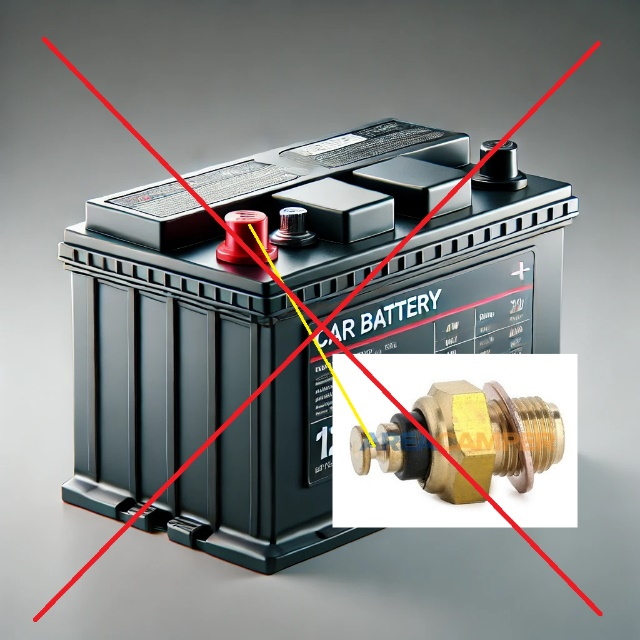
\includegraphics[width=\linewidth]{digifiz_manual/image002.jpg}
        \caption{Aviso incluido con el arnés de sensores contra la tensión externa.}
    \end{subfigure}
    \caption{Carteles de seguridad suministrados con el kit de cableado.}
\end{figure}

\chapter{Introducción}\label{ch:introduction}

Este manual operativo cubre los cuadros de instrumentos digitales \ReplicaGenOne{} y \ReplicaNextLong{} para los vehículos Volkswagen Golf~II, Jetta~II y Scirocco~II. Resume las variantes de hardware, describe sus funciones y explica cómo instalar, configurar, operar, almacenar y mantener los tableros. Las recomendaciones están dirigidas a propietarios de vehículos, electricistas automotrices y talleres que realizan la instalación del producto.

Los capítulos siguientes presentan el esquema de identificación del producto, los diagramas de pines de los conectores, las condiciones de funcionamiento y procedimientos detallados de instalación y configuración. También se incluyen referencias de mantenimiento y resolución de problemas para ambas generaciones de Replica, de modo que el cuadro pueda ser atendido sin la documentación de fábrica.

\begin{figure}[htbp]
    \centering
    \begin{subfigure}{0.48\textwidth}
        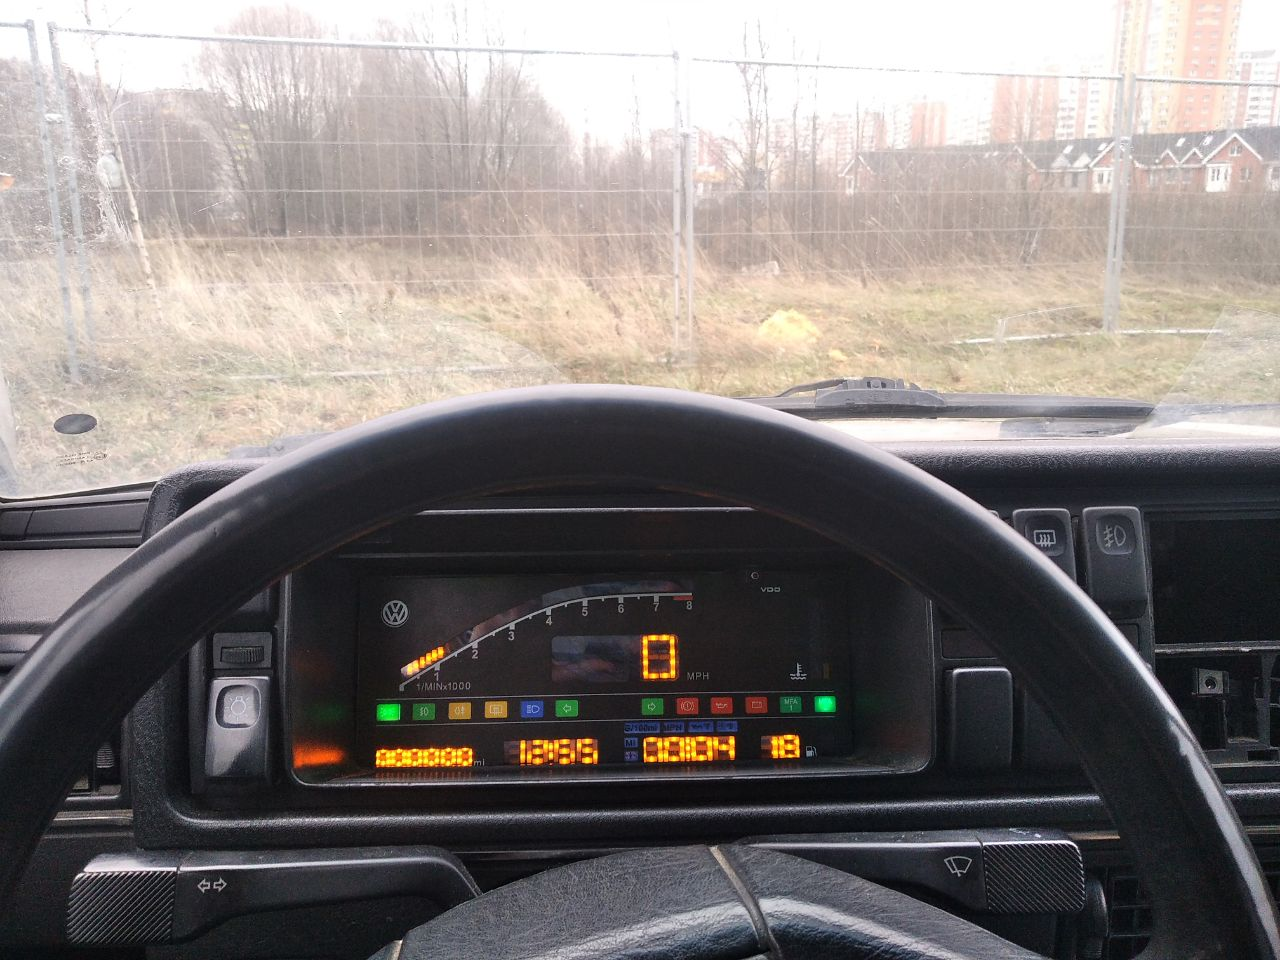
\includegraphics[width=\linewidth]{digifiz_manual/image004.jpg}
        \caption{Delivery set for the GART~8--MGF configuration.}
    \end{subfigure}\hfill
    \begin{subfigure}{0.48\textwidth}
        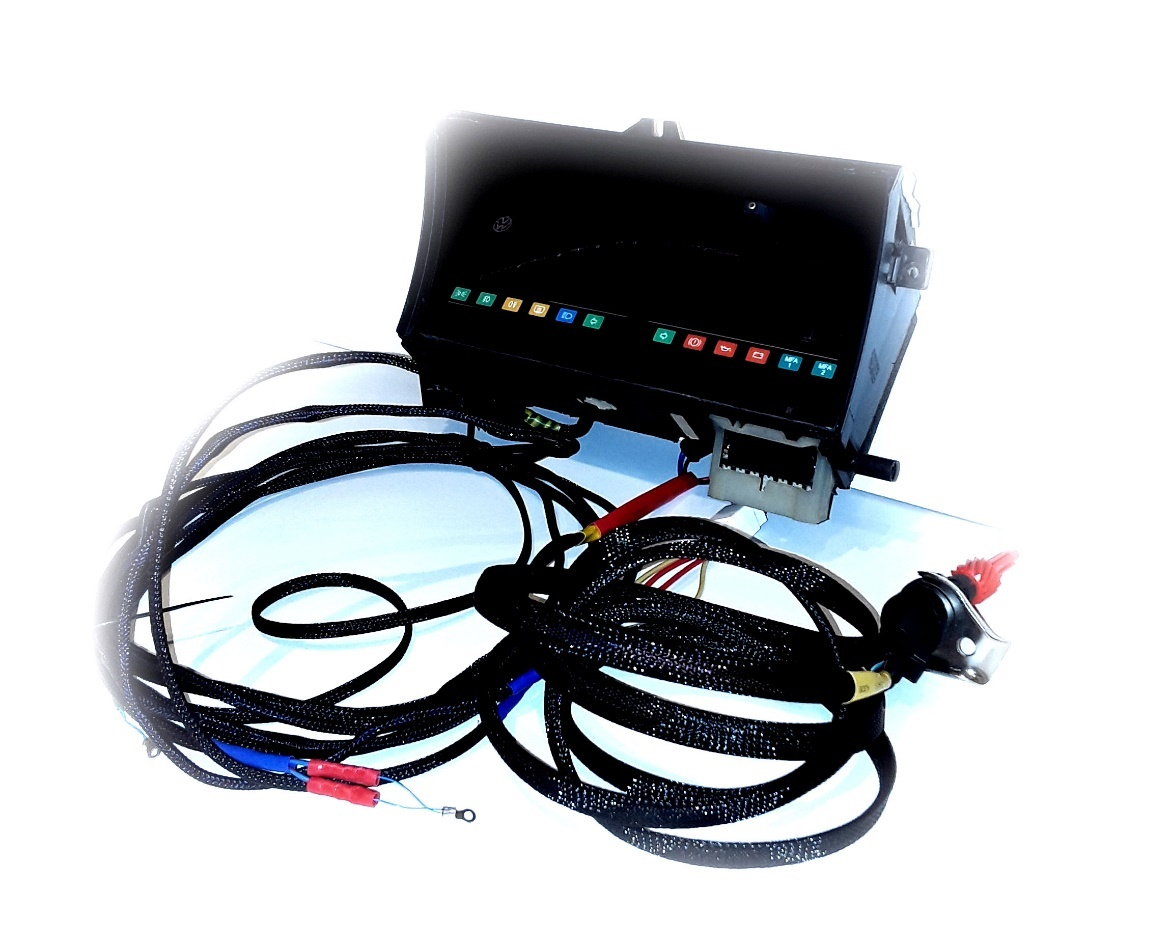
\includegraphics[width=\linewidth]{digifiz_manual/image005.jpg}
        \caption{Typical contents of a GART package.}
    \end{subfigure}
    \begin{subfigure}{0.48\textwidth}
        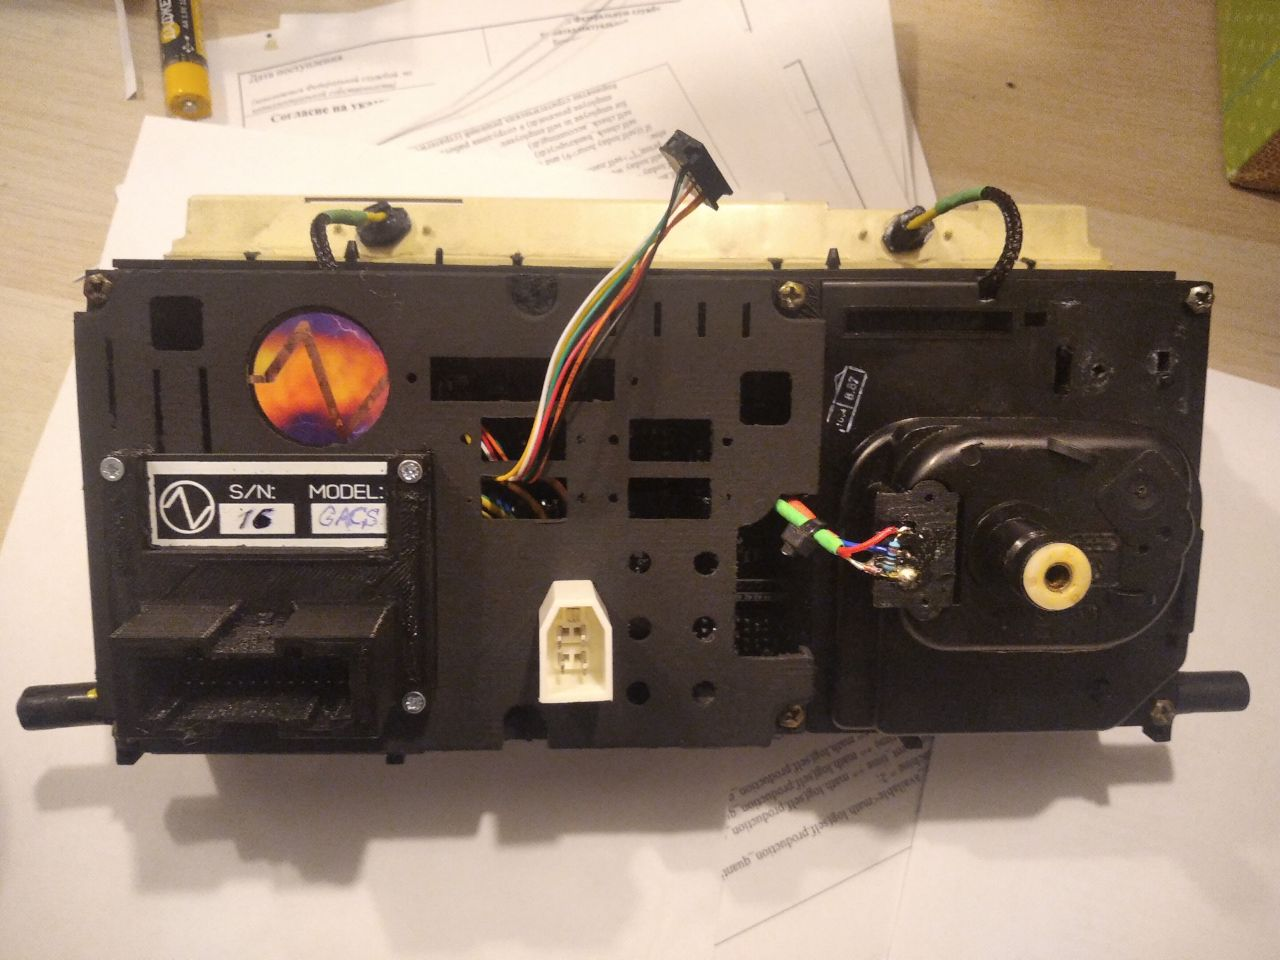
\includegraphics[width=\linewidth]{digifiz_manual/image006.jpg}
        \caption{Rear view of the single-connector GACS assembly.}
    \end{subfigure}\hfill
    \begin{subfigure}{0.48\textwidth}
        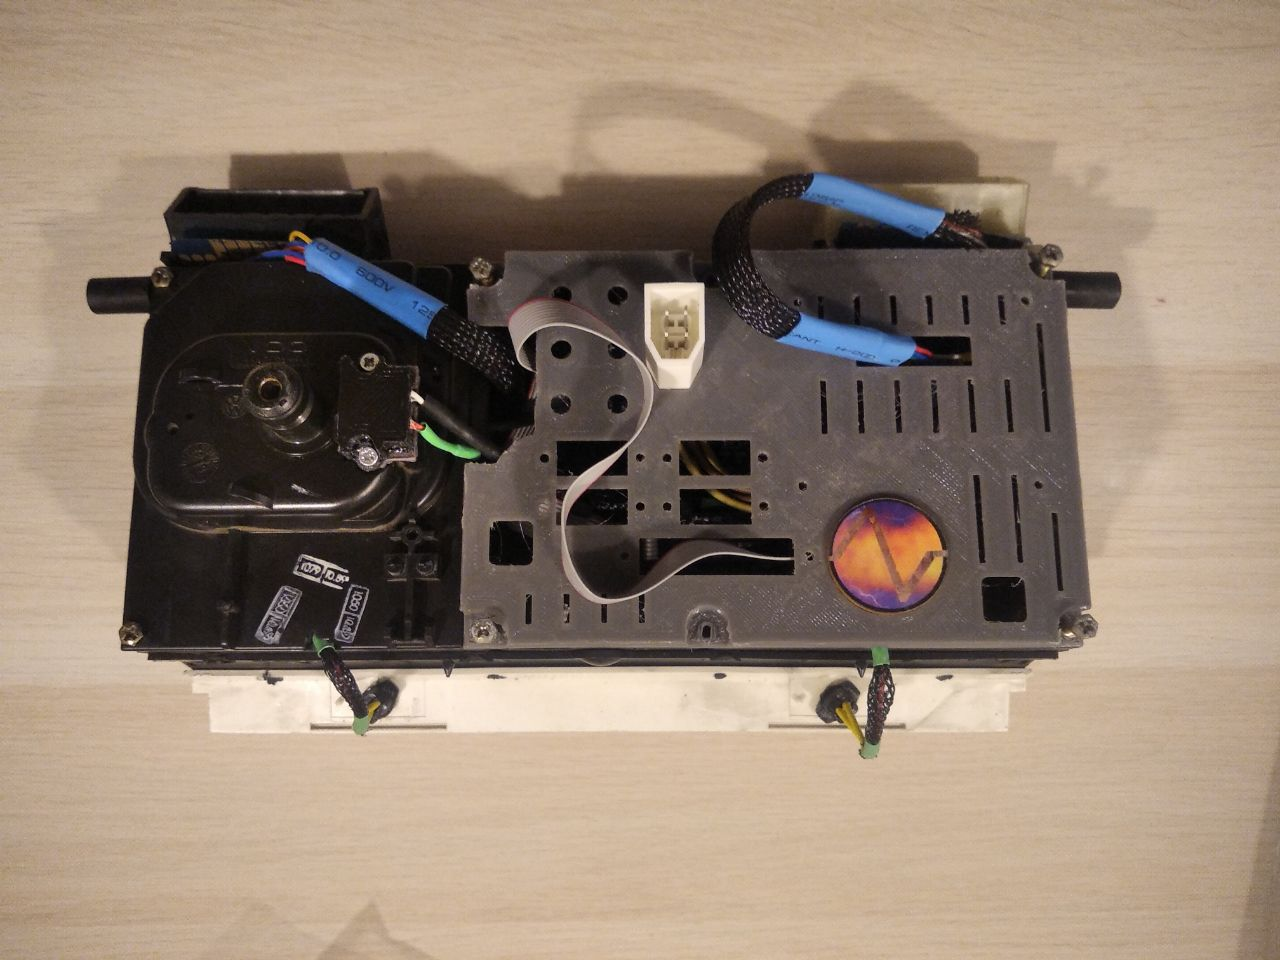
\includegraphics[width=\linewidth]{digifiz_manual/image007.jpg}
        \caption{Rear view of the dual-connector GACT assembly.}
    \end{subfigure}
    \caption{Cuadros \ReplicaGenOne{} y \ReplicaNextLong{} representativos suministrados con este manual.}
\end{figure}

Cada variante se entrega con los componentes necesarios para la cadena cinemática prevista, las unidades de medida y el estilo del mazo de cables. Los capítulos posteriores descifran los marcados de variante y proporcionan tablas de conectores para que el cuadro pueda integrarse de forma segura.

\chapter{Descripción y funcionamiento del producto}\label{ch:description}

\section{Finalidad}
Los cuadros \ReplicaGenOne{} y \ReplicaNextLong{} sustituyen a los conjuntos de instrumentos originales de Volkswagen y amplían su funcionalidad. Ofrecen indicaciones digitales de velocidad, régimen del motor, temperatura del refrigerante, nivel de combustible y cálculos auxiliares de la MFA, y son compatibles tanto con sensores de velocidad por cable como electrónicos. Las unidades \ReplicaGenOneShort{} integran un controlador Bluetooth, mientras que \ReplicaNextShort{} añade módulos de configuración mediante Wi-Fi y unidades de expansión opcionales.

\section{Identificación del modelo}
Cada cuadro está marcado con un código de cuatro letras que describe la cadena cinemática, el tipo de montaje, la interfaz del sensor de velocidad y la generación del mazo. Dígitos opcionales indican la escala admitida del cuentarrevoluciones, y un sufijo adicional de tres letras informa sobre las unidades de medida para exportación.

\subsection{Designación de cuatro letras}
\begin{description}
    \item[Posición~1] \textbf{G} para motores de gasolina o \textbf{D} para motores diésel.
    \item[Posición~2] \textbf{A} para unidades ensambladas en fábrica o \textbf{M} para kits de autoensamblaje.
    \item[Posición~3] \textbf{C} para sensor de velocidad mecánico por cable o \textbf{R} para sensor de velocidad electrónico.
    \item[Posición~4] \textbf{T} para el mazo anterior al facelift (CE~1) o \textbf{S} para el mazo posterior (CE~2).
\end{description}
Un dígito final indica la velocidad máxima mostrada del motor en miles de RPM (por ejemplo, “8” en un cuadro GACT8 equivale a una escala de 8000~RPM).

\subsection{Sufijo de unidades}
Las variantes de exportación pueden añadir un sufijo de tres letras formado a partir del conjunto \texttt{MGFK}:
\begin{description}
    \item[M] millas por hora,
    \item[G] galones,
    \item[F] Fahrenheit,
    \item[K] Kelvin.
\end{description}
Por ejemplo, un cuadro \texttt{GART8-MGF} es una unidad de gasolina, ensamblada en fábrica, con sensor electrónico, mazo CE~2, tacómetro de 8000~RPM y unidades de medida imperiales.

\section{Gama de modelos}
{\scriptsize
\begin{tblr}{
    colspec={Q[l,2.2cm] X[l]},
    hlines
}
\textbf{Modelo} & \textbf{Descripción} \\
GACT & Gasolina, completamente ensamblado, sensor de velocidad por cable, dos conectores, escala de 7000~RPM. \\
GART & Gasolina, completamente ensamblado, sensor de velocidad electrónico remoto, dos conectores, escala de 7000~RPM. \\
GAC & Gasolina, completamente ensamblado, sensor de velocidad por cable, un conector, escala de 7000~RPM. \\
GARS & Gasolina, completamente ensamblado, sensor de velocidad electrónico remoto, un conector, escala de 7000~RPM. \\
GACT8 & Gasolina, completamente ensamblado, sensor de velocidad por cable, dos conectores, escala de 8000~RPM. \\
GART8 & Gasolina, completamente ensamblado, sensor de velocidad electrónico remoto, dos conectores, escala de 8000~RPM. \\
GACS8 & Gasolina, completamente ensamblado, sensor de velocidad por cable, un conector, escala de 8000~RPM. \\
GARS8 & Gasolina, completamente ensamblado, sensor de velocidad electrónico remoto, un conector, escala de 8000~RPM. \\
DACT & Diésel, completamente ensamblado, sensor de velocidad por cable, dos conectores, escala de 6000~RPM. \\
DART & Diésel, completamente ensamblado, sensor de velocidad electrónico remoto, dos conectores, escala de 6000~RPM. \\
DACS & Diésel, completamente ensamblado, sensor de velocidad por cable, un conector, escala de 6000~RPM. \\
DARS & Diésel, completamente ensamblado, sensor de velocidad electrónico remoto, un conector, escala de 6000~RPM. \\
MT & Kit de autoensamblaje con dos conectores. \\
M.S. & Kit de autoensamblaje con un conector. \\
NEXT-GART & \ReplicaNextLong{}, escala de 8000~RPM, dos conectores, sensor de velocidad electrónico. \\
NEXT-GARS & \ReplicaNextLong{}, escala de 8000~RPM, un conector, sensor de velocidad electrónico. \\
NEXT-MT & Kit de autoensamblaje \ReplicaNextLong{} con dos conectores. \\
NEXT-MS & Kit de autoensamblaje \ReplicaNextLong{} con un conector. \\
\end{tblr}}

\section{Asignación de pines de los conectores}
\subsection{Cuadros con dos conectores}
\begin{figure}[htbp]
    \centering
    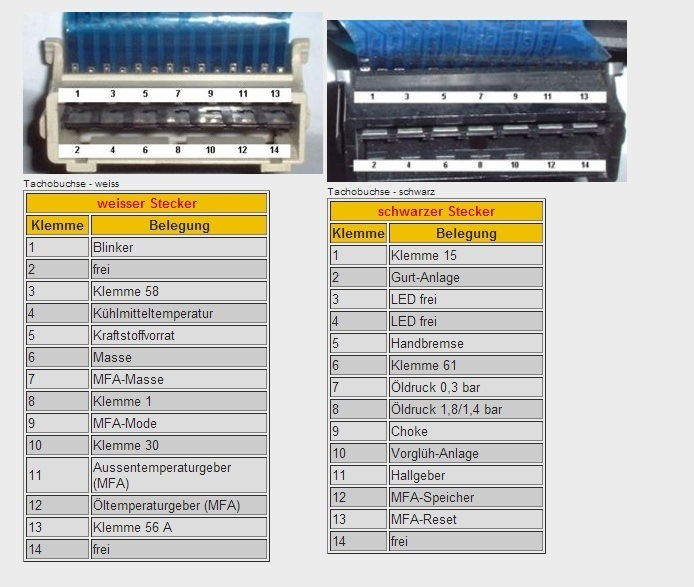
\includegraphics[width=0.72\textwidth]{digifiz_manual/image008.jpg}
    \caption{Distribución de conectores para cuadros \ReplicaGenOne{} con dos enchufes.}
\end{figure}

\noindent\textbf{Conector blanco}

{\scriptsize
\begin{tblr}{
    colspec={Q[l,1.4cm] X[l]},
    hlines
}
\textbf{Pin} & \textbf{Asignación} \\
1 & Salida de intermitente, conectada a masa para la lámpara indicadora. \\
2 & Frei — sin conexión. \\
3 & Terminal~58, alimentación positiva para la retroiluminación del panel. \\
4 & Entrada del sensor resistivo de temperatura del refrigerante. \\
5 & Entrada del sensor resistivo del nivel de combustible. \\
6 & Retorno de masa. \\
7 & Retorno de masa adicional. \\
8 & Señal de régimen del motor en el terminal~1 (bobina, distribuidor u otra forma de onda de hasta 12~V con posibles picos de 300~V). \\
9 & Línea de modo MFA utilizada para cambiar las funciones de la MFA. \\
10 & Alimentación positiva permanente UNR (sin uso en \ReplicaGenOneShort{}, alimentación principal en \ReplicaNextShort{}). \\
11 & Conductor “+” de temperatura MFA para el sensor ambiental (\ReplicaNextShort{}). \\
12 & Conductor del sensor de temperatura de aceite MFA (solo \ReplicaNextShort{}). \\
13 & Entrada del indicador de luces largas KL~56a (+12~V activo). \\
\end{tblr}}

\noindent\textbf{Conector negro}

{\scriptsize
\begin{tblr}{
    colspec={Q[l,1.4cm] X[l]},
    hlines
}
\textbf{Pin} & \textbf{Asignación} \\
1 & Terminal~15, +12~V conmutados desde el interruptor de encendido. \\
2--4 & Sin conexión. \\
5 & Entrada del indicador de freno de mano (activo en bajo). \\
6 & Salida de la lámpara de advertencia del generador KL~61 con resistencia de excitación de 120~\ensuremath{\Omega}. \\
7 & Interruptor de presión de aceite, 0.3~bar. \\
8 & Interruptor de presión de aceite, 1.8~bar. \\
9 & Sin uso. \\
10 & Entrada del indicador de precalentamiento (+12~V activo, solo diésel). \\
11 & Entrada de sensor Hall para sensores de velocidad opcionales. \\
12 & Línea de selección de bloque MFA. \\
13 & Línea de reinicio MFA. \\
\end{tblr}}

\subsection{Cuadros con un solo conector}
Los cuadros con un único conector utilizan la asignación mostrada en \autoref{fig:single-connector}. El mazo reproduce las mismas señales presentes en las variantes de dos conectores, pero las concentra en un único enchufe.

\begin{figure}[htbp]
    \centering
    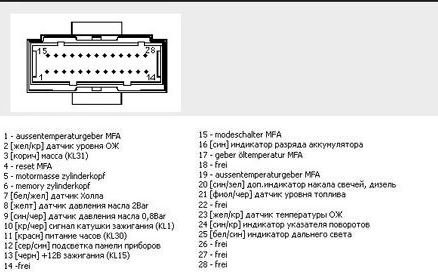
\includegraphics[width=0.65\textwidth]{digifiz_manual/image009.png}
    \caption{Distribución de un solo conector utilizada en los cuadros Replica compactos.}
    \label{fig:single-connector}
\end{figure}

\subsection{Mazo prospectivo Scirocco/Passat}
El mazo prospectivo para Scirocco/Passat utiliza dos conectores. Sus funciones se resumen a continuación.

\noindent\textbf{Conector de 5 pines}
{\scriptsize
\begin{tblr}{
    colspec={Q[l,2.6cm] X[l]},
    hlines
}
\textbf{Pin} & \textbf{Asignación} \\
1~(D3) & Contacto del indicador de la gama “D” de la transmisión automática. Conecta a masa la lámpara de marcha cuando el selector está en posición~D. \\
2~(D2) & Contacto del indicador de la segunda gama de la transmisión automática. Conecta a masa la lámpara “2” cuando el selector está en posición~2. \\
3~(D1) & Contacto del indicador de la gama baja de la transmisión automática. Conecta a masa la lámpara “1” cuando el selector está en posición~1. \\
4~(SA) & Alimentación común para la indicación del selector automático (\emph{Schaltanzeige}); proporciona los +12~V para las lámparas de gama. \\
5~(SPERRE) & Contacto del bloqueo de arranque proveniente del selector. Cerrado en estacionamiento o punto muerto para permitir el arranque del motor. \\
\end{tblr}}

\noindent\textbf{Conector de 14 pines}
{\scriptsize
\begin{tblr}{
    colspec={Q[l,2.6cm] X[l]},
    hlines
}
\textbf{Pin} & \textbf{Asignación} \\
1~(KL~58) & Alimentación de iluminación para la retroiluminación del panel. \\
2~(MASS) & Retorno de masa del chasis. \\
3~(TANK) & Entrada del aforador de combustible. \\
4~(TEMP) & Entrada del sensor de temperatura del refrigerante. \\
5~(KL~1) & Señal de régimen del motor (terminal~1). \\
6~(UHR) & +12~V permanente para el reloj y la memoria. \\
7~(FERNL) & Entrada del indicador de luces largas. \\
8~(reserved) & Sin conexión. \\
9~(OEL~1.8) & Interruptor de alta presión de aceite, 1.8~bar. \\
10~(CAT~VORGL(-)) & Entrada de la lámpara de precalentamiento catalítico / precalentamiento diésel (activa en bajo). \\
11~(OEL~0.3) & Interruptor de baja presión de aceite, 0.3~bar. \\
12~(KL~61) & Lámpara de advertencia del alternador y alimentación de excitación. \\
13~(KL~49a) & Alimentación combinada del indicador de intermitentes. \\
14~(KL~15) & Alimentación +12~V conmutada por el encendido. \\
\end{tblr}}

\subsection{Asignación de conectores para Mk1}
Los vehículos Volkswagen Mk1 utilizan las siguientes asignaciones:
\begin{enumerate}
    \item Alimentación de iluminación y luces de cruce.
    \item Referencia de masa MASSE~31.
    \item Aforador de combustible TANK.
    \item Sensor de temperatura TEMP.
    \item Señal de cuentarrevoluciones KL~1.
    \item +12~V permanente UHR.
    \item Señal de luces largas KL~56.
    \item Interruptor de presión de aceite (ALTA) 1.8~bar.
    \item Interruptor de presión de aceite (BAJA) 0.3~bar.
    \item Indicador de precalentamiento diésel.
    \item Entrada CHOKE (sin uso).
    \item Lámpara del generador KL~61.
    \item Entrada del intermitente (combinado izquierda/derecha).
    \item Alimentación de encendido KL~15.
\end{enumerate}
\begin{figure}[htbp]
    \centering
    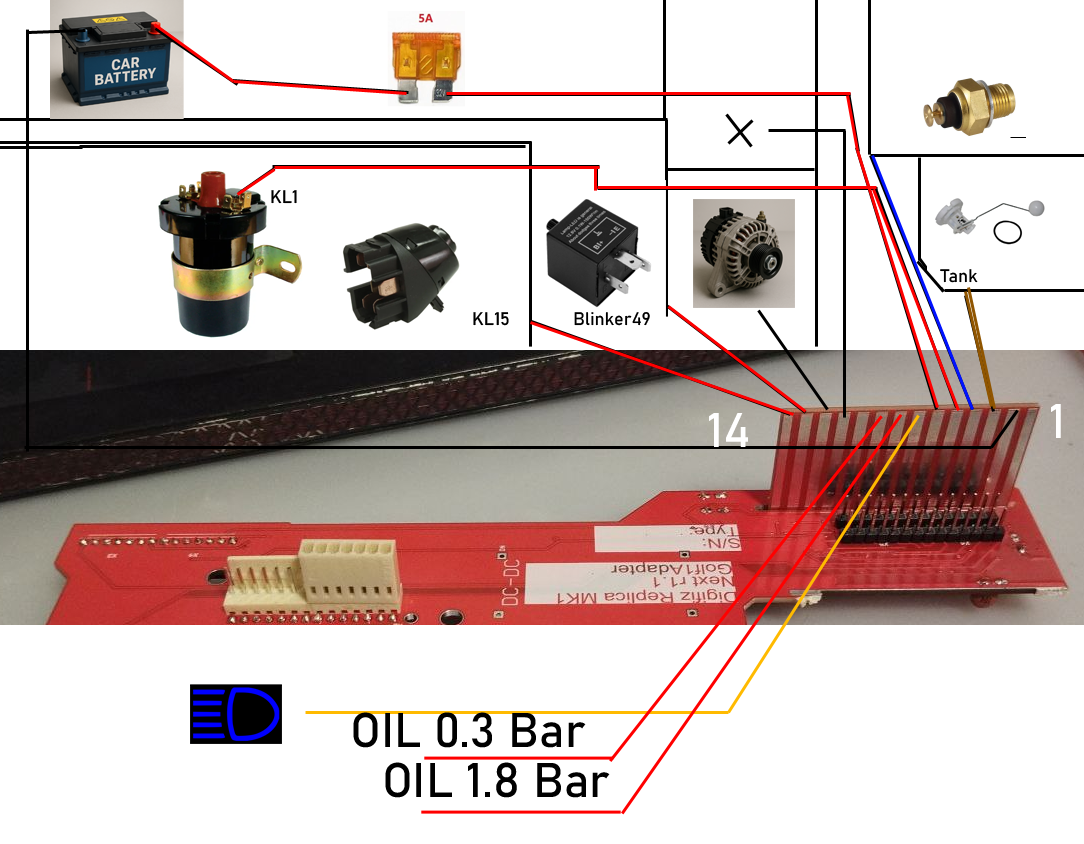
\includegraphics[width=0.75\textwidth]{digifiz_manual/image010.png}
    \caption{Diagrama de conexión del mazo para instalaciones Mk1.}
\end{figure}

\subsection{Conector de servicio de la placa de circuito impreso}
El tercer conector de la placa replica los conectores del cuadro, con pines numerados de derecha a izquierda en las unidades \ReplicaGenOneShort{} y \ReplicaNextShort{}. Proporciona una interfaz de servicio con las asignaciones listadas en \autoref{tab:service-connector}.

\begin{table}[htbp]
    \centering
    \caption{Asignaciones del conector de servicio.}
    \label{tab:service-connector}
    {\scriptsize
    \begin{tblr}{
        colspec={Q[l,1.9cm] X[l]},
        hlines,
    }
        \textbf{Posición} & \textbf{Asignación} \\
        1 & Salida de indicador. \\
        2 & Entrada del sensor de velocidad (SPM\_M). \\
        3 & Masa del vehículo. \\
        4 & Salida de indicador. \\
        5 & Entrada del optoacoplador del intermitente izquierdo. \\
        6 & Entrada del optoacoplador del intermitente derecho. \\
        7 & +12~V de encendido. \\
        8 & Entrada específica para diésel. \\
        9 & Entrada de indicador (positiva). \\
        10 & Entrada alternativa de RPM (sin uso, solo \ReplicaNextShort{}). \\
        11 & \ReplicaGenOneShort{}: salida de indicador (normalmente desconectada); \ReplicaNextShort{}: entrada de freno (activa en bajo). \\
        12 & Reservado. \\
        13 & Entrada de check engine. \\
        14 & Sin contacto. \\
    \end{tblr}}
\end{table}

\subsection{Conectores de expansión auxiliares}
En la placa principal se instalan tres cabeceras adicionales de cuatro pines para simplificar las ampliaciones del mazo y los trabajos de servicio:
\begin{itemize}
    \item \textbf{Señales analógicas de expansión:} proporciona un punto de conexión dedicado para entradas analógicas adicionales al integrar sensores personalizados.
    \item \textbf{Espejo de la MFA:} duplica el conector \textsc{MFA} estándar para admitir la derivación en paralelo de las señales del ordenador de viaje.
    \item \textbf{Duplicados analógicos:} repite las entradas de temperatura de aceite, temperatura ambiente e indicador de freno para que estos circuitos puedan rutearse a módulos externos de registro o monitorización.
\end{itemize}
Los tres utilizan el conector \mbox{KF2510-4p}, que no se suministra con el kit del cuadro y debe adquirirse por separado en caso necesario.

\begin{figure}[htbp]
    \centering
    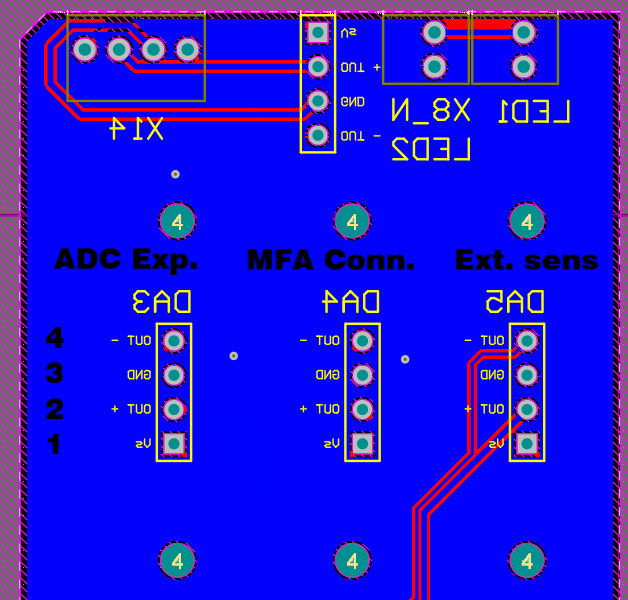
\includegraphics[width=0.6\textwidth]{digifiz_manual/ext_conn.png}
    \caption{Distribución de los conectores auxiliares en la placa principal.}
\end{figure}

\begin{table}[htbp]
    \centering
    {\small
    \begin{tblr}{
        colspec={Q[l,2.3cm] Q[c,1.3cm] X[l]},
        hlines,
        row{1} = {font=\bfseries}
    }
    Conector & Pin & Asignación \\
    Conector~I & 4 & Entrada analógica auxiliar~1 \\
    Conector~I & 3 & Masa (GND) \\
    Conector~I & 2 & Entrada analógica auxiliar~2 \\
    Conector~I & 1 & VCC (3V3, sin fusible\textbf{!!!}) \\
    Conector~II & 4 & Reinicio MFA \\
    Conector~II & 3 & Masa (GND) \\
    Conector~II & 2 & Bloque de memoria MFA \\
    Conector~II & 1 & Modo MFA \\
    Conector~III & 4 & Salida del sensor de temperatura de aceite \\
    Conector~III & 3 & Masa (GND) \\
    Conector~III & 2 & Salida del sensor de temperatura exterior \\
    Conector~III & 1 & Indicador de freno \\
    \end{tblr}}
    \caption{Asignaciones de los conectores de expansión auxiliares.}
\end{table}

\section{Software integrado y contenido del suministro}
El firmware del cuadro se publica en la siguiente dirección:
\displayurl{https://github.com/Sgw32/DigifizReplica}
Hay dos juegos de entrega disponibles:
\begin{itemize}
    \item \textbf{\ReplicaGenOne{}:} conjunto del cuadro, mazo de temperaturas ambiente y de aceite, programador USBasp y, para sensores remotos, mazo del sensor de velocidad.
    \item \textbf{\ReplicaNextLong{}:} conjunto del cuadro y mazo del sensor de velocidad electrónico.
\end{itemize}

\chapter{Principio de funcionamiento} \label{ch:operating-principle}

Los cuadros \ReplicaGenOne{} reutilizan la carcasa original de Volkswagen, los conectores de fábrica CE~1 o CE~2 y, según la configuración, el cable mecánico del velocímetro o un sensor de velocidad electrónico.
Las placas principales \ReplicaGenOneShort{} se basan en un PCB de fibra de vidrio poblado con componentes discretos controlados por un microcontrolador ATmega~2560 y controladores de indicadores MAX~7219.

\ReplicaNextLong{} se basa en un sistema en chip ESP32-S3 e introduce una carcasa de nueva fabricación impresa en SLA, un panel frontal y una tapa rediseñados, y una placa adaptadora de conectores.
La pantalla \ReplicaNextShort{} se ilumina mediante LED direccionables WS2812 montados detrás del marco frontal, y el mazo correspondiente incluye el sensor de velocidad electrónico de serie.

Ambas generaciones comparten la misma disposición de pantalla y páginas MFA, lo que garantiza que los procedimientos de instalación y la operación diaria resulten familiares entre revisiones de hardware.

\chapter{Especificaciones técnicas}\label{ch:technical-specs}

El cuadro \ReplicaGenOne{} no consume corriente en reposo cuando está apagado. \ReplicaNextShort{} demanda aproximadamente 13~mA de la alimentación de +12~V con el encendido desconectado, lo que debe tenerse en cuenta cuando el vehículo permanece almacenado durante periodos prolongados. Ambas generaciones funcionan de forma fiable con el sistema eléctrico del vehículo entre 9~V y 16~V~CC.

\section{Capacidades de medición}
\begin{itemize}
    \item \textbf{Velocidad del vehículo:} medida mediante el cable de fábrica o un sensor de velocidad electrónico. El error sistemático es de 10~km/h, el error relativo es de 3~km/h y la indicación se satura en 999~km/h (o mph para unidades imperiales).
    \item \textbf{Régimen del motor:} derivado de la señal de encendido a través de una etapa con optoacoplador con una red RC de 430~nF/1.2~k\ensuremath{\Omega} y un limitador por diodo. Los errores absoluto y relativo se mantienen dentro de 200~rpm.
    \item \textbf{Nivel de combustible:} leído del aforador resistivo del depósito con una incertidumbre de aproximadamente 10~litros.
    \item \textbf{Temperatura del refrigerante:} indicada de forma cualitativa utilizando el termistor estándar conectado mediante el mazo del vehículo; no se muestran valores cuantitativos.
    \item \textbf{Cronometraje:} mantenido con una precisión de un minuto.
    \item \textbf{Testigos:} intermitentes, luces largas, advertencias de presión de aceite, estado del generador, freno de mano, luneta térmica o precalentamiento diésel y luces antiniebla delanteras y traseras.
\end{itemize}

\chapter{Condiciones de funcionamiento y precauciones de seguridad}\label{ch:safety}

\section{Límites ambientales}
\begin{itemize}
    \item El cuadro de instrumentos funciona entre \(-40\,^{\circ}\mathrm{C}\) y \(+70\,^{\circ}\mathrm{C}\) con una humedad relativa de hasta el 95~\%.
    \item El tablero puede permanecer instalado en el vehículo durante todo el año, incluso cuando el automóvil permanece estacionado por periodos prolongados.
\end{itemize}

\section{Precauciones de seguridad}
\begin{enumerate}
    \item El cuadro Digifiz es un dispositivo de bricolaje ensamblado e integrado por entusiastas. Observe las prácticas generales de seguridad eléctrica al trabajar con él.
    \item El producto está destinado a los proyectos personales de los propietarios de vehículos.
    \item Las lecturas no están certificadas ni verificadas metrológicamente, aunque corresponden a las especificaciones declaradas en el momento del lanzamiento.
    \item Utilice el tablero únicamente cuando acepte la responsabilidad de la instalación y de la seguridad vial.
    \item Si no confía en los datos mostrados, verifíquelos con los indicadores estándar del vehículo o con instrumentos de medición externos.
    \item No utilice las salidas del cuadro de instrumentos para sistemas de control automático del vehículo.
    \item Los autores no aceptan responsabilidad por las consecuencias derivadas de la instalación o el uso del tablero, incluidas multas de tráfico o accidentes. Las averías comunicadas dentro del periodo de garantía (un año para instalaciones realizadas conjuntamente con los autores y dos semanas para instalaciones independientes) serán reparadas.
    \item Las capacidades funcionales enumeradas en \Cref{ch:technical-specs} están garantizadas durante un año en instalaciones supervisadas y durante dos semanas después de una instalación independiente.
\end{enumerate}

\chapter{Preparación para el trabajo y secuencia de tareas}\label{ch:preparation}

\section{Preparar el vehículo}
Siga la secuencia siguiente al sustituir el cuadro de fábrica por un tablero Digifiz:
\begin{enumerate}
    \item Retire las molduras plásticas que cubren los pedales y la parte inferior del tablero para dejar al descubierto el cuadro original.
    \item Desconecte la batería del vehículo.
    \item Desenchufe el mazo de cables del cuadro de instrumentos de fábrica.
    \item Desacople el cable mecánico del velocímetro, si está presente.
    \item Desatornille el cuadro de sus soportes y extráigalo con cuidado del vehículo.
    \item Guíe los mazos de sensores de temperatura y velocidad suministrados según sea necesario.
    \item Instale el tablero Digifiz en las guías del soporte y fíjelo con tornillos.
    \item Para \ReplicaNextLong{}, instale los sensores MFA de Volkswagen (o equivalentes) y lleve sus conductores hasta los conectores CE~1/CE~2.
    \item En los modelos \texttt{GACS}/\texttt{GARS}/\texttt{DARS}/\texttt{DACS}, conecte manualmente los cables etiquetados \texttt{MFA\_MODE}, \texttt{MFA\_RESET}, \texttt{MFA\_BLOCK} y freno de mano si el mazo del vehículo carece de estos contactos. La segunda generación \ReplicaNextShort{} conecta estas señales internamente por defecto.
    \item Conecte los mazos al cuadro.
    \item Monte el sensor de velocidad electrónico o vuelva a conectar el cable mecánico.
    \item Reinstale las molduras del tablero y la cubierta de los pedales en orden inverso.
\end{enumerate}

\section{Operación del tablero}
\begin{itemize}
    \item El cuadro se enciende automáticamente con el contacto. El interruptor de luces de posición controla la retroiluminación.
    \item Al inicio se ilumina toda la escala de velocidad mientras el autodiagnóstico estabiliza el modelo de RPM; la pantalla se estabiliza posteriormente en el régimen de ralentí actual.
    \item Una vez que el vehículo comienza a moverse, el sistema informa los parámetros descritos en \Cref{ch:technical-specs}.
\end{itemize}

\subsection{Funciones de la MFA}
Hay seis páginas MFA disponibles:
\begin{enumerate}
    \item Tiempo de funcionamiento diario.
    \item Distancia del trayecto.
    \item Consumo de combustible (no implementado en la primera revisión de Replica).
    \item Velocidad media (mostrada como el valor multiplicado por diez).
    \item Temperatura del aceite del motor (requiere mazo externo).
    \item Temperatura ambiente (requiere mazo externo).
\end{enumerate}
En los cuadros \ReplicaGenOneShort{} un punto táctil capacitivo detrás del emblema VW recorre las páginas; \ReplicaNextShort{} utiliza un interruptor externo en la columna de dirección. Las duraciones de pulsación se comportan de la siguiente manera:
\begin{itemize}
    \item Pulsación corta (\(<1\)~s): avanza a la siguiente función MFA.
    \item Pulsación media (1--3~s cuando no hay interruptor en la columna): alterna entre bloques de memoria MFA; el cambio se indica en pantalla.
    \item Pulsación larga (3--7~s): reinicia la función MFA activa (afecta al consumo, distancia del viaje, tiempo transcurrido y velocidad media).
\end{itemize}

\subsection{Distribución de retroiluminación e indicadores}
El cuadro \ReplicaGenOneShort{} ofrece un ajuste manual de brillo sobre el interruptor de luces de estacionamiento; \ReplicaNextShort{} confía en el brillo automático gobernado por un fotodiodo. Se pueden configurar anulaciones manuales mediante las interfaces de mantenimiento descritas en \Cref{ch:replica-setup,ch:replica-next-setup}.

La disposición del bloque horizontal de testigos y la leyenda en pantalla se muestran en \autoref{fig:indicator-layout}.

\begin{figure}[htbp]
    \centering
    \begin{subfigure}{0.48\textwidth}
        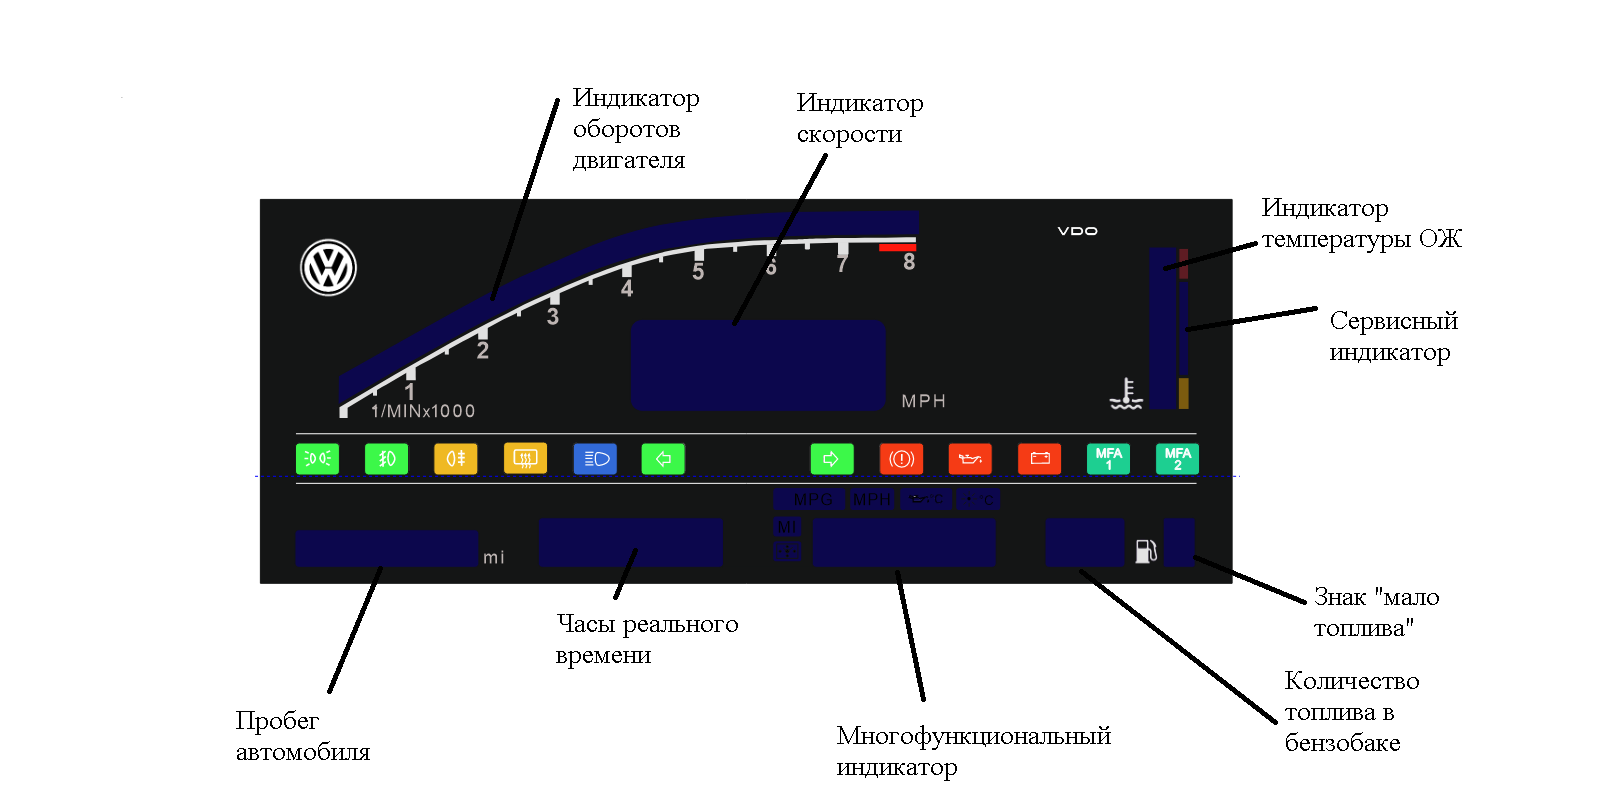
\includegraphics[width=\linewidth]{digifiz_manual/image017.png}
        \caption{Disposición de testigos mostrada durante la autocomprobación de encendido.}
    \end{subfigure}\hfill
    \begin{subfigure}{0.48\textwidth}
        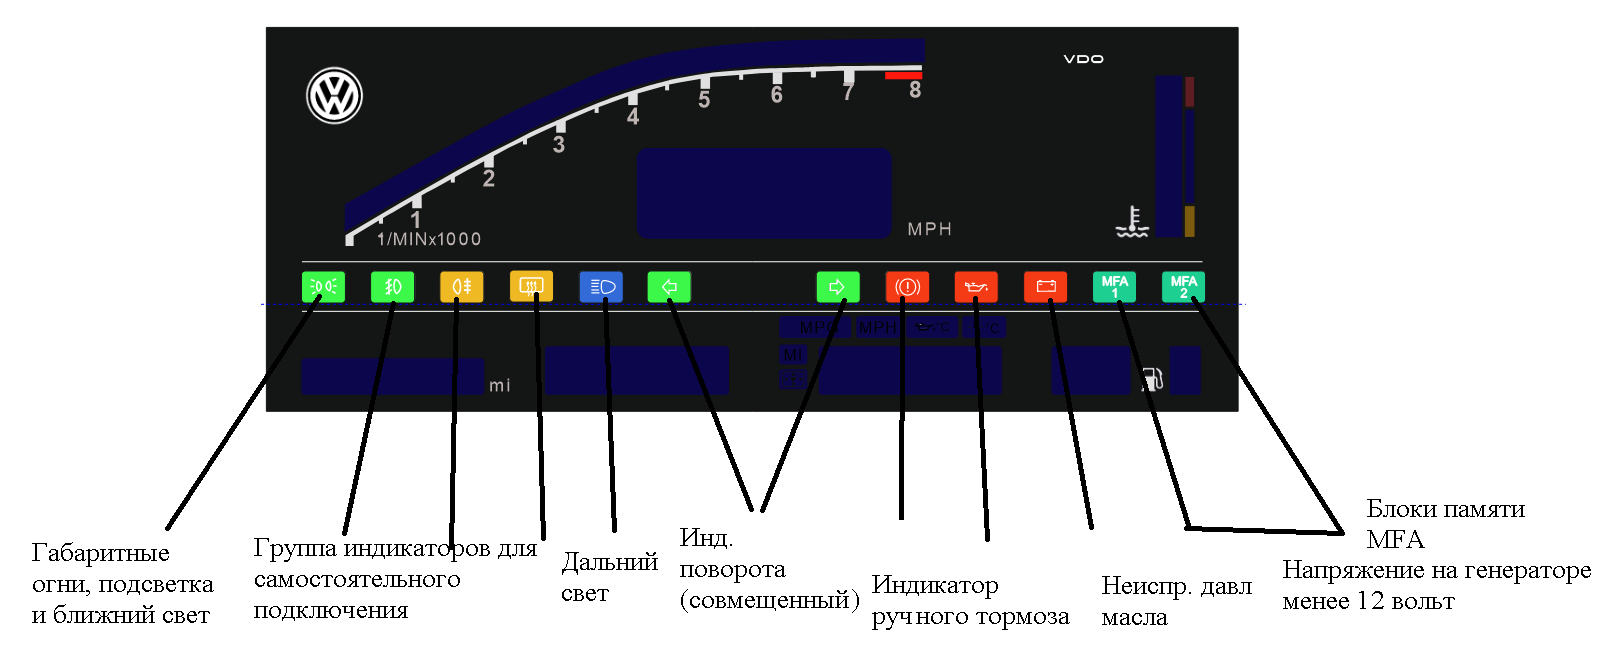
\includegraphics[width=\linewidth]{digifiz_manual/image018.png}
        \caption{Leyenda del grupo horizontal de indicadores.}
    \end{subfigure}
    \caption{Esquema de indicación del cuadro de instrumentos.}
    \label{fig:indicator-layout}
\end{figure}

\subsection{Interfaces de configuración}
\begin{itemize}
    \item Las unidades \ReplicaGenOne{} clásicas incluyen un módulo Bluetooth 2.0 (o compatible con BLE). Instale la aplicación \emph{Serial Bluetooth Terminal} desde Google Play, empareje con el cuadro y ejecute comandos directamente desde la vista de terminal. Los dispositivos Apple iOS no pueden conectarse a este módulo.
    \item \ReplicaNextShort{} expone un punto de acceso Wi-Fi integrado y un portal de configuración descrito en \Cref{ch:replica-next-setup}. Desactive los datos móviles durante la conexión para asegurarse de que el portal cautivo cargue correctamente.
\end{itemize}
Ambas generaciones pueden alimentarse y configurarse en banco utilizando la interfaz de programación USBasp.

\chapter{Configuración y mantenimiento de \ReplicaNextLong{}}\label{ch:replica-next-setup}

Esta sección se aplica al cuadro \ReplicaNextLong{} mostrado en \autoref{fig:next-hardware}.

\begin{figure}[htbp]
    \centering
    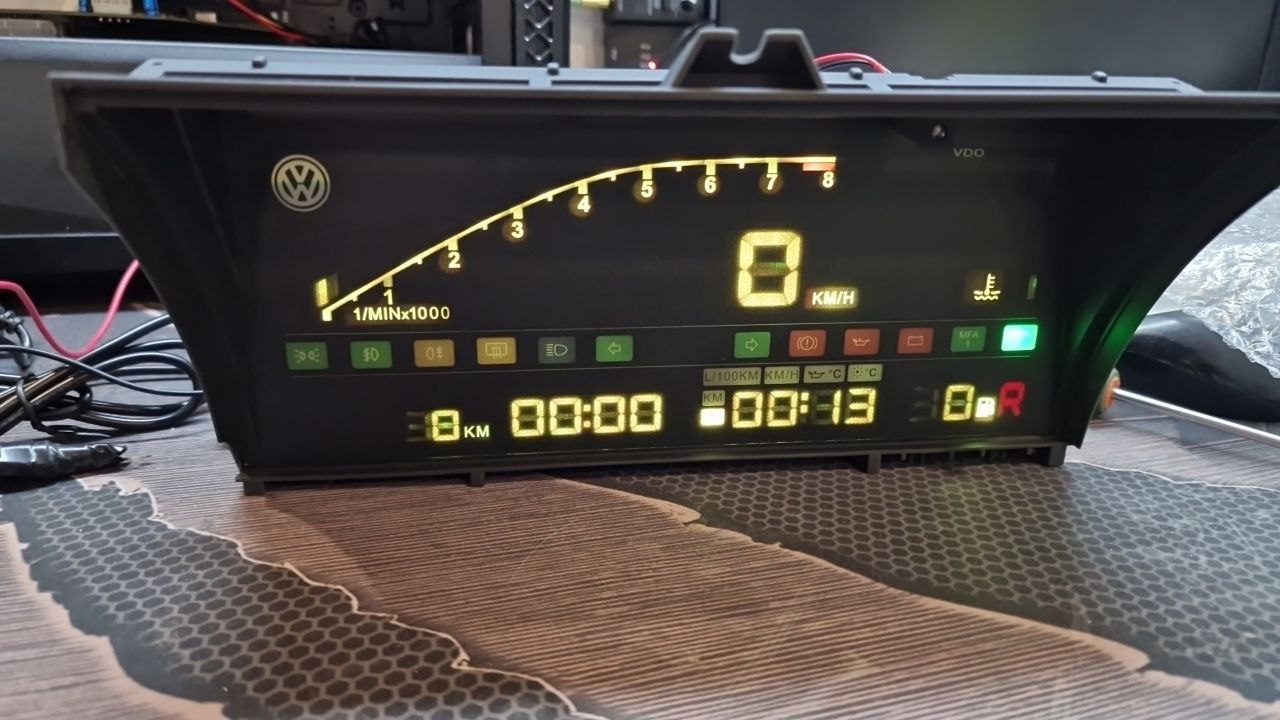
\includegraphics[width=0.6\textwidth]{digifiz_manual/image019.png}
\caption{Conjunto del cuadro \ReplicaNextLong{}.}
    \label{fig:next-hardware}
\end{figure}

\section{Manipulación del panel}
\begin{itemize}
    \item La placa frontal de policarbonato impresa en UV debe protegerse de arañazos y objetos extraños. Los daños considerables requieren piezas de repuesto de PHOL-LABS Kft y no se tratan como un caso de garantía.
    \item El reloj en tiempo real se configura mediante el panel de control Wi-Fi. Se reinicia cada vez que se desconecta la alimentación permanente.
\end{itemize}

\section{Portal de control Wi-Fi}
La configuración, la recopilación de datos y la gestión del firmware se realizan a través de la aplicación web integrada.
\begin{itemize}
    \item Conéctese al punto de acceso Wi-Fi del tablero. Desactive los datos móviles y únase a \texttt{Digifiz\_AP} (contraseña \texttt{87654321}); algunas revisiones anuncian \texttt{PHOL-LABS2} con la misma contraseña.
    \item La dirección IP predeterminada es \texttt{192.168.4.1}. Si el cuadro está configurado para unirse a otra red, escanee la subred en busca de una dirección que termine en \texttt{.32} utilizando una aplicación de herramientas IP.
    \item El portal contiene cinco pestañas: \emph{WiFi}, \emph{Control}, \emph{Settings}, \emph{Colors} y \emph{About} (\autoref{fig:next-control-tabs}). La pestaña Wi-Fi configura los ajustes de red y gestiona la carga de firmware; la pestaña Control ajusta los parámetros del cuadro; la pestaña Settings ofrece un editor estructurado para todos los parámetros del firmware; la pestaña Colors gestiona los esquemas de color multisegmento; la pestaña About muestra información de los autores.
\end{itemize}

\begin{figure}[htbp]
    \centering
    \begin{subfigure}{0.48\textwidth}
        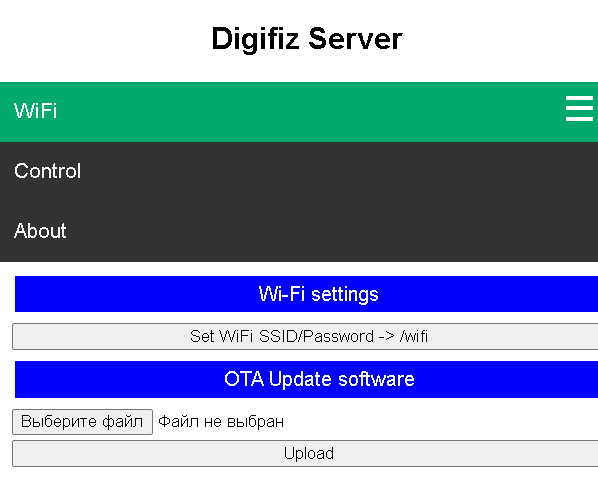
\includegraphics[width=\linewidth]{digifiz_manual/image020.png}
        \caption{Control tab overview.}
    \end{subfigure}\hfill
    \begin{subfigure}{0.48\textwidth}
        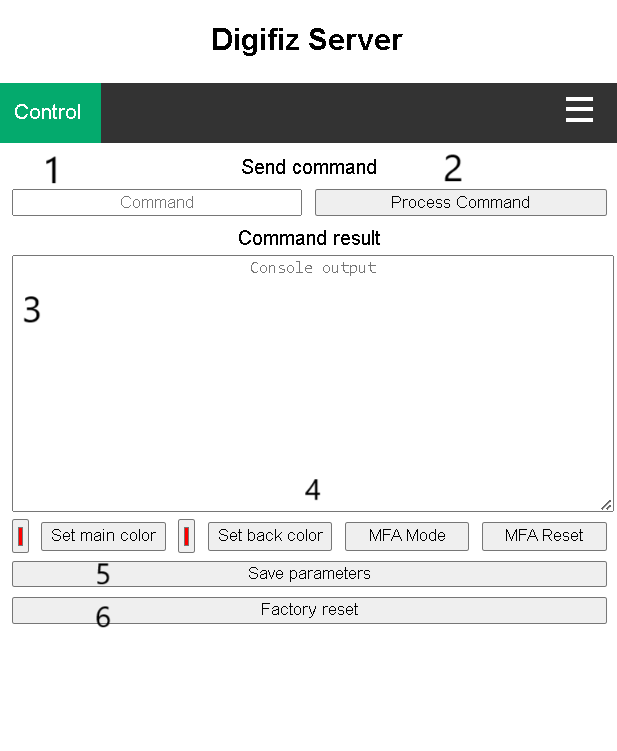
\includegraphics[width=\linewidth]{digifiz_manual/image021.png}
        \caption{Numbered controls and command entry fields.}
    \end{subfigure}
    \caption{Interfaz Wi-Fi de \ReplicaNextShort{}.}
    \label{fig:next-control-tabs}
\end{figure}

\section{Introducción de comandos}
La pestaña \emph{Control} proporciona una línea de entrada de comandos (1), un botón \emph{Process} (2), una ventana de resultados (3), controles rápidos (4), un botón \emph{Save} (5) y un botón \emph{Reset} (6). Introduzca los comandos como pares separados por espacios \verb|<número> <valor>| utilizando únicamente enteros; no se requieren signos de puntuación ni comillas. \autoref{fig:next-command-example} ilustra la interfaz al activar y desactivar el brillo automático.

\begin{figure}[htbp]
    \centering
    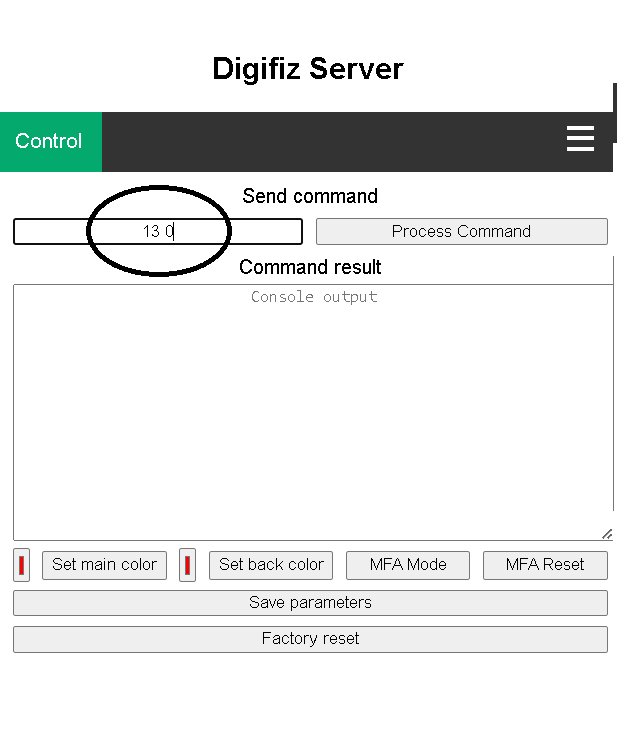
\includegraphics[width=0.55\textwidth]{digifiz_manual/image022.png}
\caption{Ejemplo de secuencia de comandos que desactiva el brillo automático.}
    \label{fig:next-command-example}
\end{figure}

\section{Referencia de comandos}
\begin{table}[htbp]
    \centering
    \caption{Comandos principales de configuración de \ReplicaNextShort{}.}
    \label{tbl:next-commands}
    {\scriptsize
    \begin{tblr}{
        colspec = {Q[c,0.14\linewidth] Q[l,0.36\linewidth] Q[l]},
        rowsep = 2pt,
    }
        \toprule
        \textbf{Comando} & \textbf{Nombre} & \textbf{Descripción} \\
        \midrule
        22 (or 0) & \paramname{PARAMETER\_RPMCOEFFICIENT} & Engine RPM calibration factor (100--10000). \\
        1  & \paramname{PARAMETER\_SPEEDCOEFFICIENT} & Factor de calibración de velocidad (10--255). \\
        2  & \paramname{PARAMETER\_COOLANTTHERMISTORB} & Coeficiente beta del termistor de refrigerante (2000--5000). \\
        3  & \paramname{PARAMETER\_OILTHERMISTORB} & Coeficiente beta del termistor de aceite (2000--5000). \\
        4  & \paramname{PARAMETER\_AIRTHERMISTORB} & Coeficiente beta del termistor ambiente (2000--5000). \\
        5  & \paramname{PARAMETER\_TANKMINRESISTANCE} & Resistencia mínima del aforador (0--1000~\ohm). \\
        6  & \paramname{PARAMETER\_TANKMAXRESISTANCE} & Resistencia máxima del aforador (100--1000~\ohm). \\
        7  & \paramname{PARAMETER\_TAU\_COOLANT} & Constante del filtro de temperatura de refrigerante (1--50; valores altos reaccionan más rápido). \\
        8  & \paramname{PARAMETER\_TAU\_OIL} & Constante del filtro de temperatura de aceite (1--50). \\
        9  & \paramname{PARAMETER\_TAU\_AIR} & Constante del filtro de temperatura ambiente (1--50). \\
        10 & \paramname{PARAMETER\_TAU\_TANK} & Constante del filtro de nivel de combustible (1--50). \\
        11 & \paramname{PARAMETER\_MILEAGE} & Valor total del odómetro (0--999999). \\
        12 & \paramname{PARAMETER\_DAILY\_MILEAGE} & Odómetro parcial (0--9999). \\
        13 & \paramname{PARAMETER\_AUTO\_BRIGHTNESS} & Activar brillo automático (1=activo, 0=desactivado). \\
        14 & \paramname{PARAMETER\_BRIGHTNESS\_LEVEL} & Nivel de brillo manual (0--60\%; valores superiores a 60 reducen la vida del LED). \\
        15 & \paramname{PARAMETER\_TANK\_CAPACITY} & Capacidad del depósito en litros (0--99; 55~L típico en Golf~2). \\
        16 & \paramname{PARAMETER\_MFA\_STATE} & Modo MFA activo (normalmente se controla por hardware). \\
        17 & \paramname{PARAMETER\_BUZZER\_OFF} & Desactivar zumbador (1 lo desactiva, 0 lo habilita; \ReplicaNextShort{} no incluye zumbador). \\
        18 & \paramname{PARAMETER\_MAX\_RPM} & Escala del cuentarrevoluciones (típico 8000, rango 4000--16000). \\
        19 & \paramname{PARAMETER\_NORMAL\_RESISTANCE\_COOLANT} & Resistencia del sensor de refrigerante a \SI{25}{\celsius} (1000--10000~\ohm). \\
        20 & \paramname{PARAMETER\_NORMAL\_RESISTANCE\_OIL} & Resistencia del sensor de aceite a \SI{25}{\celsius} (1000--10000~\ohm). \\
        21 & \paramname{PARAMETER\_NORMAL\_RESISTANCE\_AMB} & Resistencia del sensor ambiente a \SI{25}{\celsius} (1000--10000~\ohm). \\
        23 & \paramname{PARAMETER\_DOT\_OFF} & Comportamiento de los dos puntos del reloj (0=parpadeo, 1=fijo). \\
        24 & \paramname{PARAMETER\_BACKLIGHT\_ON} & Activar retroiluminación con luces de cruce (sin uso en \ReplicaNextShort{}). \\
        25 & \paramname{PARAMETER\_M\_D\_FILTER} & Constante del filtro mediano (heredado, normalmente sin uso). \\
        26 & \paramname{PARAMETER\_COOLANT\_MAX\_R} & Umbral del sensor de refrigerante para indicación a escala completa (\SI{100}{\celsius}--\SI{150}{\celsius}). \\
        27 & \paramname{PARAMETER\_COOLANT\_MIN\_R} & Umbral del sensor de refrigerante para indicación ``1~bar'' (\SI{0}{\celsius}--\SI{80}{\celsius}). \\
        31 & \paramname{PARAMETER\_MAINCOLOR\_R} & Componente roja del color de la interfaz (0--255). \\
        32 & \paramname{PARAMETER\_MAINCOLOR\_G} & Componente verde del color de la interfaz (0--255). \\
        33 & \paramname{PARAMETER\_MAINCOLOR\_B} & Componente azul del color de la interfaz (0--255). \\
        37 & \paramname{PARAMETER\_RPM\_FILTER} & Intensidad del filtro de RPM (10--200; valores altos reaccionan más rápido). \\
        128 & \paramname{PARAMETER\_READ\_ADDITION} & Sumar 128 para leer el valor actual de cualquier comando. \\
        255 & \paramname{PARAMETER\_SET\_HOUR} & Ajustar horas del reloj (formato de 24 horas). \\
        254 & \paramname{PARAMETER\_SET\_MINUTE} & Ajustar minutos del reloj. \\
        253 & \paramname{PARAMETER\_RESET\_DAILY\_MILEAGE} & Restablecer el odómetro parcial. \\
        252 & \paramname{PARAMETER\_RESET\_DIGITAL} & Restablecimiento de fábrica de los parámetros almacenados. \\
        \bottomrule
    \end{tblr}}
\end{table}

\section{Valores predeterminados}
\begin{table}[htbp]
    \centering
    \caption{Valores predeterminados de \ReplicaNextShort{}.}
    \label{tbl:next-defaults}
    {\scriptsize
    \begin{tblr}{
        colspec = {Q[l,0.42\linewidth] Q[c,0.15\linewidth] Q[l]},
        rowsep = 2pt,
    }
        \toprule
        \textbf{Parámetro} & \textbf{Predeterminado} & \textbf{Notas} \\
        \midrule
        \paramname{PARAMETER\_RPMCOEFFICIENT} & 3000 & Típico para entradas de tacómetro Audi. \\
        \paramname{PARAMETER\_SPEEDCOEFFICIENT} & 100 & Calibrado para 100~km/h. \\
        \paramname{PARAMETER\_COOLANTTHERMISTORB} & 4000 &  \\
        \paramname{PARAMETER\_OILTHERMISTORB} & 4000 &  \\
        \paramname{PARAMETER\_AIRTHERMISTORB} & 3812 & 3600 en paneles de segunda generación. \\
        \paramname{PARAMETER\_TANKMINRESISTANCE} & 35 & \ohm. \\
        \paramname{PARAMETER\_TANKMAXRESISTANCE} & 265 & \ohm. \\
        \paramname{PARAMETER\_TAU\_COOLANT} & 2 & Constante del filtro. \\
        \paramname{PARAMETER\_TAU\_OIL} & 2 & Constante del filtro. \\
        \paramname{PARAMETER\_TAU\_AIR} & 2 & Constante del filtro. \\
        \paramname{PARAMETER\_TAU\_TANK} & 2 & Constante del filtro. \\
        \paramname{PARAMETER\_MILEAGE} & Dependiente del vehículo & Mantiene el odómetro almacenado. \\
        \paramname{PARAMETER\_DAILY\_MILEAGE} & 0 &  \\
        \paramname{PARAMETER\_AUTO\_BRIGHTNESS} & 1 & Activado. \\
        \paramname{PARAMETER\_BRIGHTNESS\_LEVEL} & 25 & Predeterminado en generación~2; generación~1/1.5 usa 7 o 13. \\
        \paramname{PARAMETER\_TANK\_CAPACITY} & 63 & Litros. \\
        \paramname{PARAMETER\_MFA\_STATE} & 0 & Página MFA predeterminada. \\
        \paramname{PARAMETER\_BUZZER\_OFF} & 1 & Zumbador desactivado. \\
        \paramname{PARAMETER\_MAX\_RPM} & 8000 & Escala del cuentarrevoluciones. \\
        \paramname{PARAMETER\_NORMAL\_RESISTANCE\_COOLANT} & 1000 & \ohm{} a \SI{25}{\celsius}. \\
        \paramname{PARAMETER\_NORMAL\_RESISTANCE\_OIL} & 1000 & \ohm{} a \SI{25}{\celsius}. \\
        \paramname{PARAMETER\_NORMAL\_RESISTANCE\_AMB} & 2991 & 500~\ohm{} para sensores de segunda generación. \\
        \paramname{PARAMETER\_DOT\_OFF} & 0 & Dos puntos del reloj parpadeando. \\
        \paramname{PARAMETER\_BACKLIGHT\_ON} & 1 & Retroiluminación habilitada con luces de cruce. \\
        \paramname{PARAMETER\_M\_D\_FILTER} & 65535 & Constante heredada del filtro mediano. \\
        \paramname{PARAMETER\_COOLANT\_MAX\_R} & 120 & \si{\celsius}. \\
        \paramname{PARAMETER\_COOLANT\_MIN\_R} & 60 & \si{\celsius}. \\
        \paramname{PARAMETER\_MAINCOLOR\_R} & 180 & Valor por defecto amarillo verdoso. \\
        \paramname{PARAMETER\_MAINCOLOR\_G} & 240 & Valor por defecto amarillo verdoso. \\
        \paramname{PARAMETER\_MAINCOLOR\_B} & 6 & Valor por defecto amarillo verdoso. \\
        \paramname{PARAMETER\_RPM\_FILTER} & 70 & Respuesta del filtro. \\
        \paramname{PARAMETER\_UPTIME} & 0 & Contador de funcionamiento. \\
        \bottomrule
    \end{tblr}}
\end{table}

\section{Lectura de parámetros y ejemplos}
Para leer un parámetro, sume 128 al número de comando (por ejemplo, \verb|129 0| devuelve el coeficiente de velocidad). Entre los comandos habituales se incluyen desactivar el brillo automático (\verb|13 0|), activarlo de nuevo (\verb|13 1|), ajustar el coeficiente de velocidad (\verb|1 110| incrementa en un 10\% la velocidad mostrada) y fijar el odómetro (\verb|11 123456|). Los valores del reloj se ajustan con \verb|255 <horas>| seguido de \verb|254 <minutos>|. Los comandos 31--33 establecen los componentes RGB del color de la interfaz.

\section{Comandos de servicio}
Las revisiones recientes del firmware aceptan nombres de parámetros legibles, por ejemplo \verb|PARAMETER_RPMCOEFFICIENT 3000|. El comando de diagnóstico \verb|adc 0| muestra lecturas ADC sin procesar para diagnosticar sensores. Las actualizaciones de firmware añaden controles visuales de color, por lo que conviene actualizar periódicamente desde la pestaña \emph{WiFi} para acceder a las últimas funciones.

\section{Editor de parámetros en la pestaña Settings}
La pestaña \emph{Settings} refleja la lista de parámetros de \autoref{tbl:next-commands} y \autoref{tbl:next-defaults} e incorpora metadatos sobre rangos, descripciones y tipos de datos.
Utilícela cuando prefiera un flujo de trabajo gráfico en lugar de introducir números de comando.

\begin{enumerate}
    \item Pulse \emph{Load Parameters} para obtener los valores en vivo del cuadro. El navegador muestra cada elemento con su nombre, valor actual, descripción emergente y tipo.
    \item Para las entradas numéricas, escriba el valor deseado en la columna \emph{New Value}. La interfaz aplica el rango permitido mostrado en las columnas \emph{Min} y \emph{Max}. Los parámetros booleanos aparecen como casillas de verificación.
    \item Haga clic en \emph{Set} para enviar el cambio al instante. La tabla se actualiza para confirmar el valor modificado.
    \item Repita el proceso para cada parámetro que desee ajustar. Cuando termine, vuelva a la pestaña \emph{Control} y pulse \emph{Save parameters} para guardar la configuración en la memoria no volátil.
\end{enumerate}

El flujo de trabajo de colores exige habilitar la marca de firmware responsable de las paletas personalizadas antes de ir a la pestaña \emph{Colors}.
Busque la entrada booleana denominada “Custom colour scheme” (publicada como \verb|PARAMETER_CUSTOM_COLORSCHEME_ENABLE| en la lista de parámetros), marque la casilla y pulse \emph{Set}. El cuadro rechazará modificaciones personalizadas de segmentos hasta que esta marca esté activada.

\section{Esquemas de color personalizados}
La pestaña \emph{Colors} incorpora un editor por segmentos para la retroiluminación LED WS2812. Cada fila describe un punto final del rango, el área funcional correspondiente y el color o la herencia de un color base.

\begin{enumerate}
    \item Pulse \emph{Load Scheme} para leer el mapeo activo. Utilice \emph{Add Segment}, o los controles integrados ``+\textuparrow{}'' y ``+\textdownarrow{}'', para insertar nuevos rangos. Los menús desplegables seleccionan la función del instrumento y el selector de color base permite reutilizar los colores principal o de fondo en lugar de definir un valor RGB fijo.
    \item Haga clic en el selector de color para ajustar el tono RGB de los segmentos configurados como ``Custom''. El editor muestra los valores de los componentes en tiempo real.
    \item Use las flechas de reordenación para que coincida la secuencia física de los LED (los segmentos deben permanecer en orden ascendente). Elimine filas redundantes con el botón ``\texttimes{}''.
    \item Cuando la tabla refleje la distribución deseada, pulse \emph{Set Scheme}. El navegador recorre las filas y envía cada segmento al cuadro.
    \item Cambie inmediatamente a la pestaña \emph{Control} y pulse \emph{Save parameters}. Este paso es obligatorio: el firmware almacena los segmentos cargados en la RAM y los descarta tras un reinicio si no se guardan.
    \item Opcionalmente exporte la representación JSON mediante \emph{Export to File} para crear copias de seguridad, o importe un archivo guardado previamente con \emph{Import from File}. El botón \emph{Reset Scheme} restaura el diseño de fábrica tras confirmar la acción.
\end{enumerate}

Si posteriormente desactiva la marca de esquemas de color personalizados en la pestaña \emph{Settings}, el cuadro volverá al modo clásico de color único controlado por \verb|PARAMETER_MAINCOLOR_R/G/B|.

\chapter{Typical situations for setting up the \ReplicaNextShort{}}\label{ch:replica-next-scenarios}

\begin{description}
    \item[Hotspot not visible] Move closer to the vehicle and ensure it is parked in an open area. Disable mobile data, forget stale Wi-Fi profiles, and reconnect to \texttt{Digifiz\_AP} (or \texttt{PHOL-LABS2}).
    \item[404 at \texttt{192.168.4.1}] Turn off mobile data on the phone or laptop and reload the page. Captive portal detection on Android/iOS often interferes until the cellular modem is disabled.
    \item[Firmware updates] Open the \emph{WiFi} tab and select the supplied \texttt{Digifiz.bin} file. The latest releases are published at the link below.
        \displayurl{https://github.com/Sgw32/DigifizReplica/releases}
        Click \emph{Upload}. The first attempt can fail; repeat the upload if necessary. Successful flashes redirect to a confirmation page. Record the odometer before updating and restore it afterwards with \verb|11 <mileage>|.
    \item[Commands ignored] Refresh the browser, return to the \emph{Control} tab, and resend the command. Ensure the \emph{Process} button is pressed after entering the value.
    \item[Speed reading incorrect] Connect via Wi-Fi, drive at an indicated \SI{100}{\kilo\metre\per\hour}, note the GPS speed, then issue \verb|1 <gps_value>| (for example, \verb|1 85|) to set \paramname{PARAMETER\_SPEEDCOEFFICIENT} to the verified value.
    \item[RPM reading incorrect] Adjust \paramname{PARAMETER\_RPMCOEFFICIENT}. Older firmware uses \verb|0 <value>|; current versions use \verb|22 <value>|. Example: \verb|22 1500| halves the reading relative to \verb|22 3000|.
    \item[Display too dim] Disable automatic brightness with \verb|13 0|, then raise the manual level (for example, \verb|14 50|). Experiment with values between 45 and 55; avoid levels above 60 to preserve LED life.
    \item[Setting the clock] Use the web terminal (or Serial Bluetooth Terminal on legacy builds) to send \verb|255 <hours>| followed by \verb|254 <minutes>|. Example: \verb|255 23| and \verb|254 55| sets 23:55.
    \item[Fuel readings stuck] Disconnect the battery and measure the resistance between the fuel sender pin and vehicle ground. Valid readings are typically \SIrange{30}{300}{\ohm}. Repair shorts below \SI{5}{\ohm} or open circuits before reconnecting. If the readings vary correctly but the gauge does not, record \verb|adc 0| results at several fuel levels and share them with PHOL-LABS Kft.
    \item[Fuel flow readings inaccurate] The optional flow sensor produces emulated data and is unreliable without an intake manifold pressure sensor. Treat the readings as experimental.
    \item[Coolant temperature out of range] Tune \paramname{PARAMETER\_COOLANT\_MIN\_R} and \paramname{PARAMETER\_COOLANT\_MAX\_R}. Example: \verb|27 30| lowers the ``1~bar'' threshold to \SI{30}{\celsius}.
    \item[Oil or ambient temperature missing] With the battery disconnected and the engine cold, measure the sensor resistance. Oil sensors should read about \SI{2}{\kilo\ohm} \ensuremath{\pm}\SI{0.3}{\kilo\ohm}, ambient sensors about \SI{10}{\kilo\ohm} \ensuremath{\pm}\SI{2}{\kilo\ohm}. Adjust \paramname{PARAMETER\_NORMAL\_RESISTANCE\_OIL} (command~20) or \paramname{PARAMETER\_NORMAL\_RESISTANCE\_AMB} (command~21); lower values decrease the indicated temperature, higher values increase it. Persistent issues should be diagnosed by collecting \verb|adc 0| output and contacting PHOL-LABS Kft.
    \item[Changing interface colour] Use commands 31--33 to set the RGB values. New firmware revisions include visual colour controls in the web interface, so update regularly.
\end{description}

\chapter{Configuración y mantenimiento de \ReplicaGenOne{}}\label{ch:replica-setup}

Este capítulo se aplica al cuadro clásico \ReplicaGenOne{} mostrado en \autoref{fig:replica-classic}. Si su tablero coincide con la disposición de \ReplicaNextLong{}, consulte el capítulo anterior.

\begin{figure}[htbp]
    \centering
    \begin{subfigure}{0.46\textwidth}
        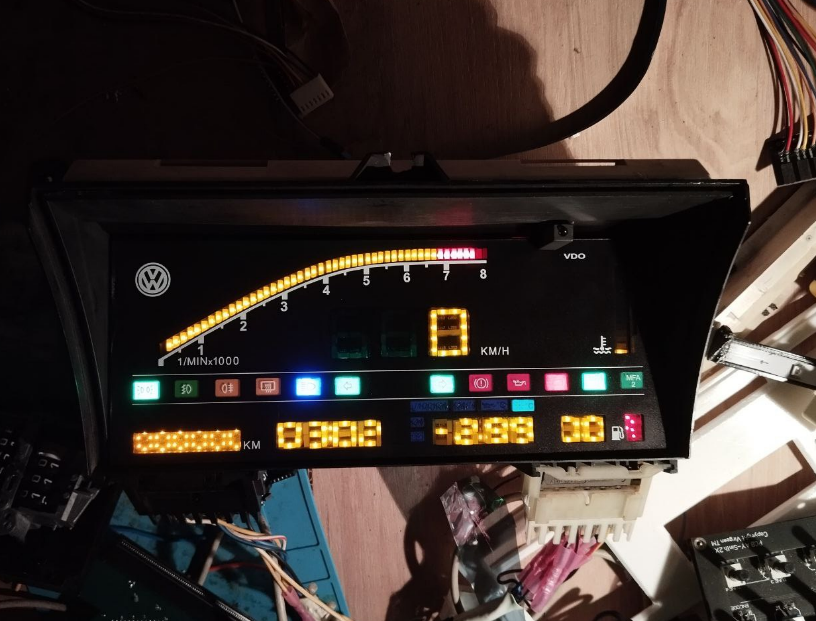
\includegraphics[width=\linewidth]{digifiz_manual/image046.png}
        \caption{Classic \ReplicaGenOne{} with square bezel.}
    \end{subfigure}\hfill
    \begin{subfigure}{0.46\textwidth}
        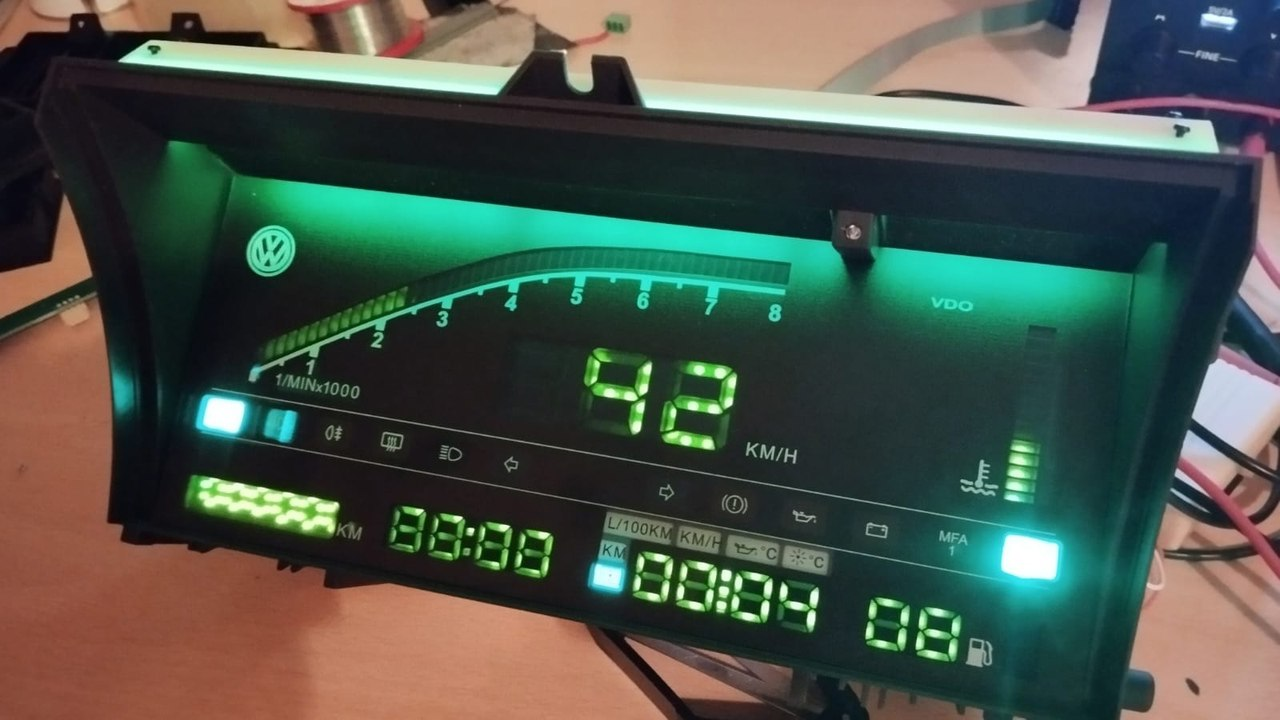
\includegraphics[width=\linewidth]{digifiz_manual/image047.png}
        \caption{Round-edge fascia used on later kits.}
    \end{subfigure}
    \caption{Aspecto del cuadro \ReplicaGenOne{}.}
    \label{fig:replica-classic}
\end{figure}

\section{Manipulación y cuidado de la pantalla}
\begin{itemize}
    \item La parte frontal de plexiglás con impresión UV se marca con facilidad. Evite el contacto con objetos punzantes o abrasivos.
    \item Los daños superficiales son cosméticos y no están cubiertos por la garantía. Solicite piezas de repuesto a PHOL-LABS Kft si el patrón de la pantalla se deforma.
\end{itemize}

\section{Batería del reloj en tiempo real}
El cuadro incorpora un reloj en tiempo real DS3231 con una pila CR2032. La batería suele durar alrededor de cuatro años. Cuando se agota, el reloj se reinicia en cada encendido. Retire la tapa frontal y/o trasera, mantenga conectados los mazos de cables y sustituya la pila tipo botón. Deseche la batería usada según la normativa local.

\section{Mantenimiento de firmware con USBasp}
Cada kit se entrega con un cable de programador USBasp ya conectado dentro de la carcasa (\autoref{fig:usbasp-cable}). Instale un controlador USBasp adecuado antes de grabar. Por ejemplo, descárguelo en la siguiente dirección:
\displayurl{https://myrobot.ru/downloads/driver-usbasp-v-2.0-usb-isp-windows-7-8-10-xp.php}
El programador alimenta el cuadro cuando se conecta a un ordenador, lo que permite realizar pruebas en banco.

\begin{figure}[htbp]
    \centering
    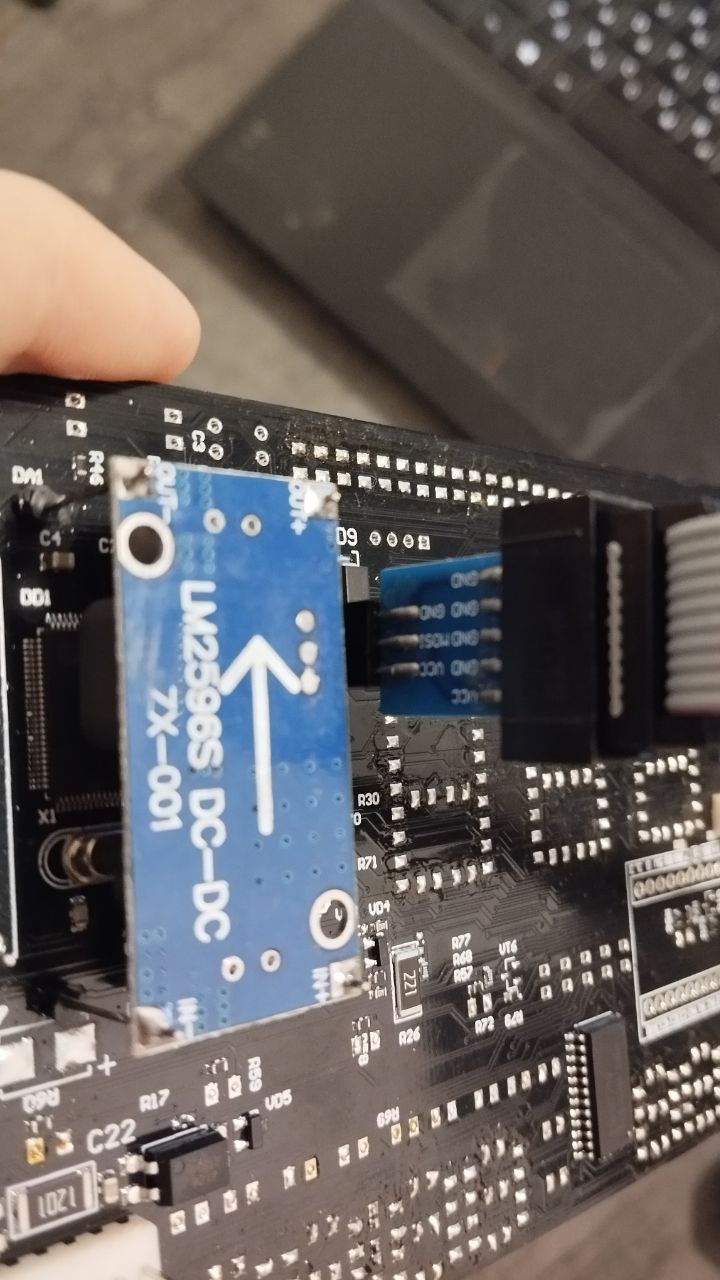
\includegraphics[width=0.32\textwidth]{digifiz_manual/image048.png}
    \caption{Orientación del mazo USBasp dentro del \ReplicaGenOne{}.}
    \label{fig:usbasp-cable}
\end{figure}

Grabe el firmware con \texttt{avrdude} mediante el comando siguiente (sustituya el nombre del archivo si es necesario):

\begin{verbatim}
avrdude -c usbasp -p m2560 -e \
    -U lfuse:w:0xff:m -U hfuse:w:0x99:m -U efuse:w:0xff:m \
    -U flash:w:Digifiz.ino.mega.hex
\end{verbatim}

Después de una carga correcta pulse el botón táctil frontal cuatro o cinco veces para inicializar los bloques de memoria. Si los bloques siguen vacíos, repita el proceso de grabación o envíe el comando Bluetooth \verb|252 0| para ejecutar un restablecimiento de fábrica. Las imágenes de firmware listas para usar se publican en:
\displayurl{https://github.com/Sgw32/DigifizReplica}

\section{Configuración por Bluetooth}
La mayoría de los parámetros se ajustan mediante Bluetooth usando un teléfono Android y la aplicación Serial Bluetooth Terminal. Descárguela del enlace siguiente antes de emparejar con el cuadro:
\displayurl{https://play.google.com/store/apps/details?id=de.kai_morich.serial_bluetooth_terminal&hl=en&gl=US}
Los dispositivos iOS no pueden conectarse al módulo Bluetooth 2.0 clásico.

\begin{itemize}
    \item Ensure you pair with the dashboard's Bluetooth Classic interface rather than BLE-only devices.
    \item In Serial Bluetooth Terminal set the end-of-line character to LF. Disable CR+LF before sending commands.
\end{itemize}

\begin{figure}[htbp]
    \centering
    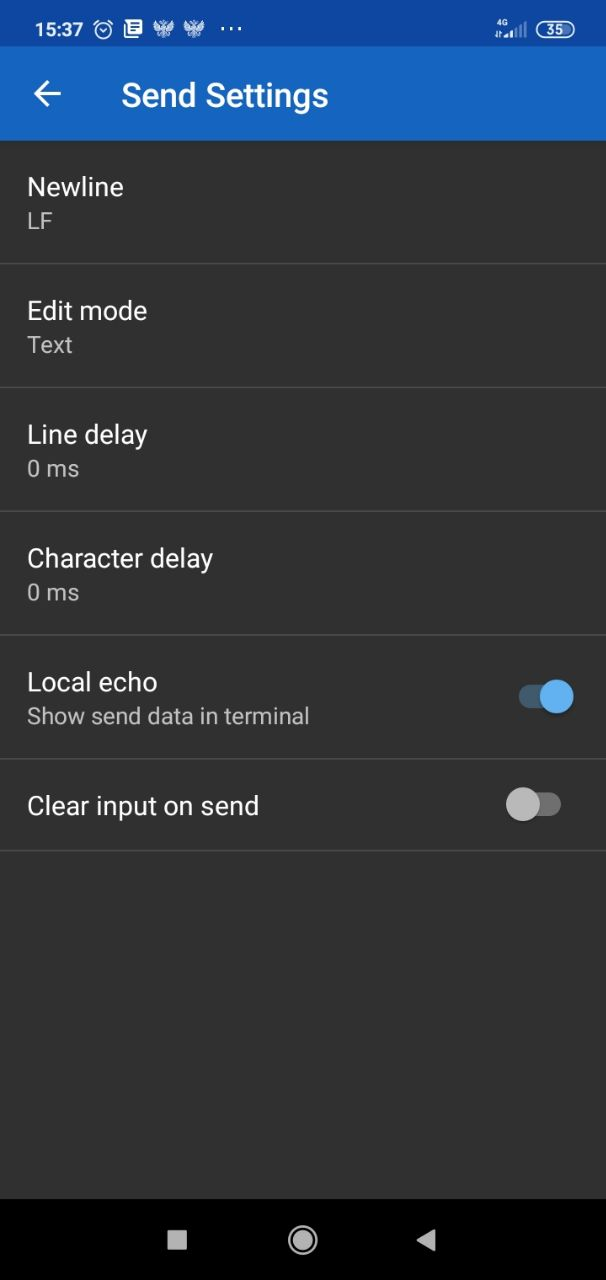
\includegraphics[width=0.32\textwidth]{digifiz_manual/image049.png}
    \caption{Configuración recomendada de Serial Bluetooth Terminal.}
    \label{fig:sbt-settings}
\end{figure}

Introduzca los comandos como pares separados por espacios \verb|<número> <valor>|. Por ejemplo, para guardar un odómetro de 123\,456~km envíe \verb|11 123456|. Sume 128 al número de comando para leer su valor actual (\verb|129 0| devuelve el coeficiente de velocidad). El comando de diagnóstico \verb|adc 0| muestra lecturas sin procesar de los sensores que ayudan a los desarrolladores a analizar fallos.

\section{Parámetros de configuración}
Los comandos Bluetooth principales se enumeran en \autoref{tbl:replica-classic-commands}. Los ajustes predeterminados para los cuadros de las generaciones~1/1.5 y~2 se resumen en \autoref{tbl:replica-defaults}. Utilice los comandos~31--33 solo en unidades \ReplicaNextShort{}; no tienen efecto en el \ReplicaGenOneShort{} clásico.

{\scriptsize
\begin{longtblr}[
    caption = {Comandos de configuración del \ReplicaGenOne{} clásico.},
    label = {tbl:replica-classic-commands},
]{
    colspec = {Q[c,0.14\linewidth] >{\ttfamily}Q[l,0.38\linewidth] Q[l]},
    rowsep = 2pt,
}
    \toprule
    \textbf{ID} & \textbf{Nombre} & \textbf{Descripción} \\
    \midrule
    22 (o 0) & PARAMETER\_RPMCOEFFICIENT & Factor de calibración de RPM del motor. \\
    1 & PARAMETER\_SPEEDCOEFFICIENT & Factor de calibración de velocidad. \\
    2 & PARAMETER\_COOLANTTHERMISTORB & Coeficiente beta del termistor de refrigerante. \\
    3 & PARAMETER\_OILTHERMISTORB & Coeficiente beta del termistor de aceite. \\
    4 & PARAMETER\_AIRTHERMISTORB & Coeficiente beta del termistor ambiente. \\
    5 & PARAMETER\_TANKMINRESISTANCE & Resistencia mínima del aforador (\si{\ohm}). \\
    6 & PARAMETER\_TANKMAXRESISTANCE & Resistencia máxima del aforador (\si{\ohm}). \\
    7 & PARAMETER\_TAU\_COOLANT & Constante del filtro de temperatura de refrigerante. \\
    8 & PARAMETER\_TAU\_OIL & Constante del filtro de temperatura de aceite. \\
    9 & PARAMETER\_TAU\_AIR & Constante del filtro de temperatura ambiente. \\
    10 & PARAMETER\_TAU\_TANK & Constante del filtro de nivel de combustible. \\
    11 & PARAMETER\_MILEAGE & Valor total del odómetro. \\
    12 & PARAMETER\_DAILY\_MILEAGE & Odómetro parcial. \\
    13 & PARAMETER\_AUTO\_BRIGHTNESS & Activar ajuste automático de brillo. \\
    14 & PARAMETER\_BRIGHTNESS\_LEVEL & Nivel de brillo manual (0--15). \\
    15 & PARAMETER\_TANK\_CAPACITY & Capacidad del depósito (litros). \\
    16 & PARAMETER\_MFA\_STATE & Página MFA activa. \\
    17 & PARAMETER\_BUZZER\_OFF & Desactivar el zumbador (1 desactiva, 0 habilita). \\
    18 & PARAMETER\_MAX\_RPM & Escala del cuentarrevoluciones (8000 por defecto). \\
    19 & PARAMETER\_NORMAL\_RESISTANCE\_COOLANT & Resistencia del sensor de refrigerante a \SI{25}{\celsius}. \\
    20 & PARAMETER\_NORMAL\_RESISTANCE\_OIL & Resistencia del sensor de aceite a \SI{25}{\celsius}. \\
    21 & PARAMETER\_NORMAL\_RESISTANCE\_AMB & Resistencia del sensor ambiente a \SI{25}{\celsius}. \\
    23 & PARAMETER\_DOT\_OFF & Comportamiento de los dos puntos del reloj (0 parpadeo, 1 fijo). \\
    24 & PARAMETER\_BACKLIGHT\_ON & Encender la retroiluminación con las luces de cruce. \\
    25 & PARAMETER\_M\_D\_FILTER & Constante del filtro mediano (heredado). \\
    26 & PARAMETER\_COOLANT\_MAX\_R & Umbral de temperatura de refrigerante para escala completa. \\
    27 & PARAMETER\_COOLANT\_MIN\_R & Umbral de temperatura de refrigerante para ``1~bar''. \\
    31--33 & PARAMETER\_MAINCOLOR\_[RGB] & Componentes de color de la interfaz (solo \ReplicaNextShort{}). \\
    37 & PARAMETER\_RPM\_FILTER & Intensidad del filtrado de RPM. \\
    128 & PARAMETER\_READ\_ADDITION & Sumar para leer cualquier parámetro. \\
    255 & PARAMETER\_SET\_HOUR & Ajustar horas del reloj (formato 24 h). \\
    254 & PARAMETER\_SET\_MINUTE & Ajustar minutos del reloj. \\
    253 & PARAMETER\_RESET\_DAILY\_MILEAGE & Restablecer el odómetro parcial. \\
    252 & PARAMETER\_RESET\_DIGITAL & Restablecimiento de fábrica e inicialización de memoria. \\
    \bottomrule
\end{longtblr}}

Los botones rápidos de Serial Bluetooth Terminal son prácticos para acciones habituales como activar o desactivar el brillo automático (\verb|13 0| y \verb|13 1|) o escribir valores de color. Mantenga valores de brillo por encima del \SI{60}{\percent} solo durante pruebas breves para preservar la vida útil de los LED.

\chapter{Situaciones típicas al configurar \ReplicaGenOne{}}\label{ch:replica-scenarios}

Antes de realizar un diagnóstico, confirme que el cuadro corresponde al \ReplicaGenOne{} clásico (\autoref{ch:replica-setup}). Los paneles \ReplicaNextLong{} utilizan un portal Wi-Fi y se describen en \autoref{ch:replica-next-scenarios}.

\begin{description}
    \item[Módulo Bluetooth no detectado] Empareje con la interfaz Bluetooth Classic del cuadro (normalmente se anuncia como \texttt{Digifiz}). Serial Bluetooth Terminal para Android sigue siendo la herramienta recomendada: configure el carácter de fin de línea como LF y evite los escáneres solo BLE, que no pueden descubrir el módulo.
    \item[El iPhone o iPad no se conecta] Los cuadros \ReplicaGenOneShort{} utilizan Bluetooth~2.0 y no son compatibles con dispositivos iOS. Use un teléfono Android o un ordenador con una utilidad de puerto serie Bluetooth.
    \item[Comandos ignorados en firmware 2024 o posterior] Desbloquee el analizador enviando \verb|234 123| y repita la secuencia deseada. Guarde botones de acceso rápido en Serial Bluetooth Terminal para los valores que ajusta con frecuencia.
    \item[Lectura de velocidad demasiado alta o baja] Conéctese mediante Serial Bluetooth Terminal, conduzca a \SI{100}{\kilo\metre\per\hour} indicados y anote la velocidad GPS. Envíe \verb|1 <gps_value>| (por ejemplo, \verb|1 85|) para que \paramname{PARAMETER\_SPEEDCOEFFICIENT} coincida con la velocidad verificada.
    \item[Lectura de RPM incorrecta] El firmware anterior a 2024 espera \verb|0 <valor>|, mientras que las versiones actuales usan \verb|22 <valor>|. Los motores Audi suelen requerir \verb|22 3000|; reduzca o duplique el valor (por ejemplo, \verb|22 1500| o \verb|22 6000|) hasta que la pantalla coincida con el cuentarrevoluciones.
    \item[Incrementar brillo] Desactive el control automático con \verb|13 0| y aumente el nivel manual con \verb|14 <valor>|. Los valores entre 45 y 55 iluminan sensiblemente la pantalla; evite niveles superiores a 60 para preservar la vida de los LED. Reactive el fotodiodo después con \verb|13 1|.
    \item[Ajuste del reloj] Use Serial Bluetooth Terminal para enviar \verb|255 <hours>| seguido de \verb|254 <minutes>|. Ejemplos: \verb|255 23|, \verb|254 55| establece 23:55; \verb|255 14|, \verb|254 30| establece 14:30; \verb|255 2|, \verb|254 28| establece 02:28.
    \item[Problemas con el indicador de combustible] Desconecte la batería del vehículo antes de medir.\begin{itemize}
        \item Si la indicación cae de 60 a 0, mida la resistencia del aforador entre el pin del mazo y la masa; las lecturas válidas suelen estar entre \SIrange{30}{300}{\ohm}. Limpie el conector y confirme que la señal llega a la placa principal.
        \item Si el indicador queda al máximo, busque un cortocircuito a masa inferior a \SI{5}{\ohm} en la línea del aforador y repárelo.
        \item Si la lectura no cambia nunca, compare la resistencia del aforador con el depósito lleno y vacío. Sustituya el sensor si se mantiene constante.
    \end{itemize}
    \item[Valores de caudal de combustible incorrectos] El canal de caudal es emulado a menos que se instale un sensor de presión del colector de admisión. Considere la lectura como orientativa.
    \item[Indicador de refrigerante impreciso] Ajuste \paramname{PARAMETER\_COOLANT\_MIN\_R} y \paramname{PARAMETER\_COOLANT\_MAX\_R}. Ejemplo: \verb|27 30| acorta la escala para que la marca de ``1~bar'' se alinee con aproximadamente \SI{30}{\celsius}.
    \item[Faltan las lecturas de temperatura de aceite o ambiente] Una lectura de \texttt{-999} o un valor fijo indica un problema de sensor. Con la batería desconectada y el motor frío, mida la resistencia del sensor entre el pin del mazo y la masa. Los sensores de aceite deberían marcar alrededor de \SI{2}{\kilo\ohm} \ensuremath{\pm}\SI{0.3}{\kilo\ohm}; los sensores de ambiente, alrededor de \SI{10}{\kilo\ohm} \ensuremath{\pm}\SI{2}{\kilo\ohm}. Ajuste \paramname{PARAMETER\_NORMAL\_RESISTANCE\_OIL} (comando~20) o \paramname{PARAMETER\_NORMAL\_RESISTANCE\_AMB} (comando~21) si necesita afinar la indicación. Las averías persistentes deben documentarse con registros de \verb|adc 0| y escalarse al soporte de PHOL-LABS Kft.
\end{description}

Si el problema persiste, recopile datos en bruto con \verb|adc 0| y compártalos con los desarrolladores del cuadro para su análisis.

\chapter{Marking and sealing}\label{ch:marking}

\begin{itemize}
    \item Each dashboard may be marked with the model number corresponding to its instrument-cluster variant.
    \item Export batches can include additional markings applied by the importing organisation.
    \item The \ReplicaGenOne{} is not sealed; no tamper seals are fitted at the factory.
\end{itemize}

\chapter{Embalaje}\label{ch:package}

\begin{enumerate}
    \item Para el transporte, envuelva el conjunto del cuadro en plástico de burbujas y colóquelo en una caja de cartón rígida.
    \item Se acepta un embalaje alternativo siempre que proteja el tablero durante el transporte y el almacenamiento.
\end{enumerate}

\chapter{Storage and transportation rules}\label{ch:storage}

\begin{itemize}
    \item Transportation conditions must comply with the general freight rules applicable to each transport mode (GOST~23216-78).
    \item Packaged dashboards may be shipped by road, rail, river, or air transport.
    \item Store the instrument panel inside the vehicle cabin or in a heated room between \SI{15}{\celsius} and \SI{40}{\celsius}. Protect the unit from direct sunlight, although storage behind vehicle glass is permissible.
\end{itemize}


\appendix
\chapter{Tablas de referencia} \label{appendix:reference}

\section{Referencia de comandos para \ReplicaGenOne{} clásico}

El firmware clásico Replica comparte la mayoría de los comandos con \ReplicaNextShort{}.
Los comandos 31--33 (control de color) solo están activos en unidades \ReplicaNextShort{}; el resto se aplica por igual a ambas generaciones.

\begin{table}[htbp]
    \centering
    \caption{Comandos principales de configuración para cuadros \ReplicaGenOne{} clásicos.}
    \label{tbl:replica-commands}
    {\scriptsize
    \begin{tblr}{
        colspec = {>{\ttfamily}Q[c,0.12\linewidth] Q[l] Q[l]},
        rowsep = 2pt,
    }
        \toprule
        \textbf{Comando} & \textbf{Nombre} & \textbf{Descripción} \\
        \midrule
        22 (o 0) & PARAMETER\_RPMCOEFFICIENT & Factor de calibración de RPM del motor. \\
        1  & PARAMETER\_SPEEDCOEFFICIENT & Factor de calibración de velocidad. \\
        2  & PARAMETER\_COOLANTTHERMISTORB & Coeficiente beta del termistor de refrigerante. \\
        3  & PARAMETER\_OILTHERMISTORB & Coeficiente beta del termistor de aceite. \\
        4  & PARAMETER\_AIRTHERMISTORB & Coeficiente beta del termistor ambiente. \\
        5  & PARAMETER\_TANKMINRESISTANCE & Resistencia mínima del aforador. \\
        6  & PARAMETER\_TANKMAXRESISTANCE & Resistencia máxima del aforador. \\
        7--10 & PARAMETER\_TAU\_\textit{X} & Constantes de filtrado para refrigerante, aceite, aire y nivel de combustible.
        \\
        11 & PARAMETER\_MILEAGE & Valor total del odómetro. \\
        12 & PARAMETER\_DAILY\_MILEAGE & Odómetro parcial. \\
        13 & PARAMETER\_AUTO\_BRIGHTNESS & Activar brillo automático. \\
        14 & PARAMETER\_BRIGHTNESS\_LEVEL & Nivel de brillo manual. \\
        15 & PARAMETER\_TANK\_CAPACITY & Capacidad del depósito. \\
        16 & PARAMETER\_MFA\_STATE & Modo MFA activo. \\
        17 & PARAMETER\_BUZZER\_OFF & Desactivar el zumbador (solo Replica). \\
        18 & PARAMETER\_MAX\_RPM & Escalado del cuentarrevoluciones (7000 por defecto). \\
        19--21 & PARAMETER\_NORMAL\_RESISTANCE\_\textit{X} & Resistencias de sensores a \SI{25}{\celsius} para refrigerante, aceite y ambiente. \\
        23 & PARAMETER\_DOT\_OFF & Comportamiento de los dos puntos del reloj. \\
        24 & PARAMETER\_BACKLIGHT\_ON & Activar la retroiluminación con las luces de cruce. \\
        25 & PARAMETER\_M\_D\_FILTER & Constante del filtro mediano. \\
        26 & PARAMETER\_COOLANT\_MAX\_R & Umbral del sensor de refrigerante para indicación a escala completa. \\
        27 & PARAMETER\_COOLANT\_MIN\_R & Umbral del sensor de refrigerante para indicación ``1~bar''. \\
        31--33 & PARAMETER\_MAINCOLOR\_[RGB] & Componentes de color de la interfaz (solo \ReplicaNextShort{}). \\
        37 & PARAMETER\_RPM\_FILTER & Intensidad del filtrado de RPM. \\
        128 & PARAMETER\_READ\_ADDITION & Sumar 128 para leer el valor actual de un comando. \\
        255 & PARAMETER\_SET\_HOUR & Ajustar horas del reloj. \\
        254 & PARAMETER\_SET\_MINUTE & Ajustar minutos del reloj. \\
        253 & PARAMETER\_RESET\_DAILY\_MILEAGE & Restablecer el odómetro parcial. \\
        252 & PARAMETER\_RESET\_DIGITAL & Restablecimiento de fábrica de los parámetros almacenados. \\
        \bottomrule
    \end{tblr}}
\end{table}

\section{Valores predeterminados de \ReplicaGenOneShort{} clásico}

\begin{table}[htbp]
    \centering
    \caption{Configuración predeterminada para el \ReplicaGenOne{} clásico.}
    \label{tbl:replica-defaults}
    {\scriptsize
    \begin{tblr}{
        colspec = {>{\ttfamily}Q[c,0.22\linewidth] Q[c,0.16\linewidth] Q[l]},
        rowsep = 2pt,
    }
        \toprule
        \textbf{Parámetro} & \textbf{Predeterminado} & \textbf{Notas} \\
        \midrule
        PARAMETER\_RPMCOEFFICIENT & 3000 &  \\
        PARAMETER\_SPEEDCOEFFICIENT & 100 &  \\
        PARAMETER\_COOLANTTHERMISTORB & 4000 &  \\
        PARAMETER\_OILTHERMISTORB & 4000 &  \\
        PARAMETER\_AIRTHERMISTORB & 3812 & 3600 en Gen~2. \\
        PARAMETER\_TANKMINRESISTANCE & 35 & Ohmios. \\
        PARAMETER\_TANKMAXRESISTANCE & 265 & Ohmios. \\
        PARAMETER\_TAU\_COOLANT & 2 &  \\
        PARAMETER\_TAU\_OIL & 2 &  \\
        PARAMETER\_TAU\_AIR & 2 &  \\
        PARAMETER\_TAU\_TANK & 2 &  \\
        PARAMETER\_MILEAGE & Dependiente del vehículo & Conserva el odómetro existente. \\
        PARAMETER\_DAILY\_MILEAGE & 0 &  \\
        PARAMETER\_AUTO\_BRIGHTNESS & 1 & Activado. \\
        PARAMETER\_BRIGHTNESS\_LEVEL & 7 o 13 & Valores típicos para Gen~1/1.5. \\
        PARAMETER\_TANK\_CAPACITY & 63 & Litros. \\
        PARAMETER\_MFA\_STATE & 0 &  \\
        PARAMETER\_BUZZER\_OFF & 1 & Zumbador desactivado. \\
        PARAMETER\_MAX\_RPM & 8000 & 7000 en cuadros anteriores. \\
        PARAMETER\_NORMAL\_RESISTANCE\_COOLANT & 1000 & \si{\ohm} a \SI{25}{\celsius}. \\
        PARAMETER\_NORMAL\_RESISTANCE\_OIL & 1000 & \si{\ohm} a \SI{25}{\celsius}. \\
        PARAMETER\_NORMAL\_RESISTANCE\_AMB & 2991 & \si{\ohm} a \SI{25}{\celsius}. \\
        PARAMETER\_DOT\_OFF & 0 & Dos puntos parpadeando. \\
        PARAMETER\_BACKLIGHT\_ON & 1 & Activada. \\
        PARAMETER\_M\_D\_FILTER & 65535 &  \\
        PARAMETER\_COOLANT\_MAX\_R & 120 & \si{\celsius}. \\
        PARAMETER\_COOLANT\_MIN\_R & 60 & \si{\celsius}. \\
        PARAMETER\_MAINCOLOR\_[RGB] & -- & Comandos de color no activos en el Replica clásico. \\
        PARAMETER\_RPM\_FILTER & 70 &  \\
        PARAMETER\_UPTIME & 0 &  \\
        \bottomrule
    \end{tblr}}
\end{table}

\section{Registro de cambios} \label{app:change-log}

\begin{table}[htbp]
    \centering
    \caption{Hoja de registro de cambios del documento.}
    \label{tbl:change-log}
    {\scriptsize
    \begin{tblr}{
        colspec = {Q[c,0.12\linewidth] Q[l] Q[c,0.2\linewidth]},
        rowsep = 2pt,
    }
        \toprule
        \textbf{Cambio} & \textbf{Hojas afectadas} & \textbf{Fecha} \\
        \midrule
        1 & 04.10.2022 & 04~Oct~2022 \\
        2 & 31.08.2023 & 31~Aug~2023 \\
        3 & 05.08.2024 & 05~Aug~2024 \\
        4 & LaTeX document introduced. & 22.09.2025 \\
        \bottomrule
    \end{tblr}}
\end{table}


\backmatter
\references

\end{document}
